% Arquivo principal: versão adaptada ao template FCTE/UnB.
\documentclass[12pt,openright,oneside,a4paper,english,french,spanish,brazil]{abntex2}

\usepackage{ifpdf}

\usepackage{lmodern}	
\usepackage[T1]{fontenc}	
\usepackage[utf8]{inputenc}		
\usepackage{lastpage}		
\usepackage{indentfirst}
\usepackage{color}	
\usepackage{graphicx}	
\usepackage{units}
\usepackage[brazilian,hyperpageref]{backref}
\usepackage[alf,no-abnt-option-file,tcc-citacoes-autor-data]{abntex2cite}
\usepackage{bold-extra}
\usepackage{eso-pic}

\renewcommand{\backrefpagesname}{Citado na(s) página(s):~}
\renewcommand{\backref}{}
\renewcommand*{\backrefalt}[4]{
	\ifcase #1 %
		Nenhuma citação no texto.%
	\or
		Citado na página #2.%
	\else
		Citado #1 vezes nas páginas #2.%
	\fi}%
% ---


\usepackage{fixos/customizacoes}
\usepackage{longtable,booktabs,array,calc}
\usepackage{listings}
\renewcommand{\lstlistingname}{Quadro}
\lstset{
  basicstyle=\scriptsize\ttfamily,
  breaklines=true,
  breakatwhitespace=true,
  columns=flexible,
  keepspaces=true,
  showstringspaces=false
}
\usepackage{xurl}
\usepackage{tikz}
\usetikzlibrary{arrows.meta,positioning,patterns,calc}
\usepackage{pgfplots}
\pgfplotsset{compat=1.18}
\usepackage{pgf-pie}

\usepackage{etoolbox}
% Identificadores (IDs) com hiperligação interna para a linha da tabela de estudos
% (\hypertarget{estudo:ID}{ID}). Aceita vários IDs: \estudo{E05,E06}.
\makeatletter
\DeclareRobustCommand{\estudo}[1]{%
  \begingroup
  \def\estudo@sep{}%
  \def\do##1{\estudo@sep\hyperlink{estudo:##1}{##1}\def\estudo@sep{, }}%
  \docsvlist{#1}%
  \endgroup}
\makeatother
% A lista de referências indica as páginas das chamadas bibliográficas.
\renewcommand*{\backrefalt}[4]{%
  \ifcase #1 %
  \or
    Citado na página #2.%
  \else
    Citado #1 vezes nas páginas #2.%
  \fi}

\newcounter{none}
\providecommand{\tightlist}{\setlength{\itemsep}{0pt}\setlength{\parskip}{0pt}}
\ifpdf
    \usepackage{cmap}
\fi
% !TeX root = ../tcc.tex
% Dados incompletos no arquivo de origem: preencher antes da entrega.
\autor{Euller Júlio da Silva \and Gabriel Henrique Castelo Costa}
\curso{Engenharia de Software}
\titulo{Avaliação de modelos de visão computacional na identificação de padrões associados à hanseníase em imagens}
\data{2026}
\palavraChaveUm{Hanseníase}
\palavraChaveDois{Visão computacional}
\orientador{Hilmer Rodrigues Neri}
\coorientador{Vinicius de Carvalho Rispoli}
\cdu{[A preencher]}
\dataDaAprovacao{[A preencher]}
\membroConvidadoUm{[A preencher]}
\membroConvidadoDois{[A preencher]}

\local{Brasília, DF}
\instituicao{%
  Universidade de Brasília -- UnB
  \par
  Faculdade de Ciências e Tecnologias em Engenharia -- FCTE
}
\tipotrabalho{Trabalho de Conclusão de Curso}
\preambulo{Monografia submetida ao curso de graduação em \imprimircurso\ 
da Universidade de Brasília, como requisito parcial para obtenção do Título 
de Bacharel em \imprimircurso.}

\definecolor{blue}{RGB}{41,5,195}
\makeatletter
\hypersetup{
     	%pagebackref=true,
		pdftitle={\@title}, 
		pdfauthor={\@author},
    	pdfsubject={\imprimirpreambulo},
	    pdfcreator={LaTeX with abnTeX2},
		pdfkeywords={abnt}{latex}{abntex}{abntex2}{trabalho acadêmico}, 
		colorlinks=true,       		% false: boxed links; true: colored links
    	linkcolor=blue,          	% color of internal links
    	citecolor=blue,        		% color of links to bibliography
    	filecolor=magenta,      		% color of file links
		urlcolor=blue,
		bookmarksdepth=4
}
\makeatother
\setlength{\parindent}{1.3cm}
\setlength{\parskip}{0.2cm}  
\makeindex

\setsecnumdepth{subsubsection}
\settocdepth{subsubsection}
\bibliographystyle{abntex2-alf}
\begin{document}
\frenchspacing
\imprimircapa
\imprimirfolhaderosto*{\folhaderostoname}
% Os demais elementos pré-textuais foram omitidos porque não constam da fonte.
\pdfbookmark[0]{\contentsname}{toc}
\tableofcontents*
\cleardoublepage

\textual
% !TeX root = ../tcc.tex
\chapter{Introdução}

Este capítulo apresenta o contexto da aplicação de modelos de visão
computacional à identificação de manifestações dermatológicas associadas
à hanseníase. São delimitados o problema de pesquisa, a questão
norteadora e os objetivos do trabalho, considerando a avaliação de
desempenho na identificação de padrões associados à hanseníase em
imagens de pele, no contexto de apoio à triagem na rede pública de saúde
do Brasil.

\section{Contexto}\label{contexto}

A hanseníase é uma doença infecciosa causada principalmente pelo
\textit{Mycobacterium leprae} e integra o grupo das doenças tropicais
negligenciadas \estudo{E12}. Atinge sobretudo populações com pouco
acesso a serviços \estudo{E13}. Suas manifestações cutâneas incluem manchas
e úlceras (Figura~\ref{fig:lesoes-hanseniase}).

\begin{figure}[htbp]
\centering
\caption{Lesões cutâneas na hanseníase: úlcera em estágio avançado (à esquerda) e mancha hipocrômica (à direita)}
\label{fig:lesoes-hanseniase}
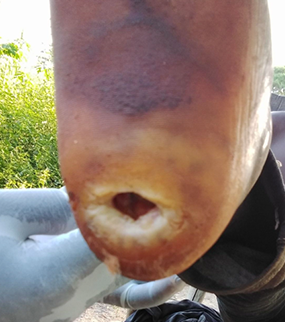
\includegraphics[height=5.2cm]{figuras/hanseniase_yotsu2023_fig2e.png}\hspace{0.8cm}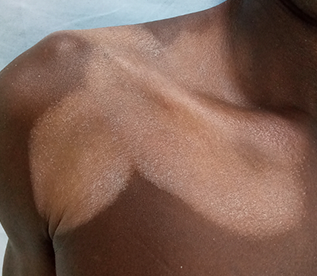
\includegraphics[height=5.2cm]{figuras/hanseniase_yotsu2023_fig2f.png}
\fonte{Adaptado de \estudo{E05}, Figura 2e e 2f (licença CC BY 4.0).}
\end{figure}

Em 2025, a Organização Mundial da Saúde
registrou 167.292 novos casos em 180 países com dados reportados; Índia
(91.783), Brasil (22.901) e Indonésia (16.292) concentram 78,3\% do total
\cite{oms2026gho}, e o Brasil é o segundo país em número de casos
(Figura~\ref{fig:casos-paises}). Na ausência de um teste diagnóstico, o diagnóstico clínico costuma ser tardio, o que
pode causar dano neurológico irreversível, com o estigma dele decorrente,
e manter a transmissão \estudo{E13}; por isso, o diagnóstico precoce é
essencial \estudo{E12}. A hanseníase constitui, assim, um desafio para a
identificação oportuna de casos e o acompanhamento das pessoas afetadas.
Em sua revisão da literatura, \estudo{E01} destaca que o diagnóstico se
baseia principalmente na avaliação clínica e que a semelhança com outras
condições dermatológicas pode dificultar o reconhecimento da doença. Em
países de baixa e média renda, os profissionais da linha de frente muitas
vezes não têm formação em dermatologia, e a Organização Mundial da Saúde
disponibilizou um aplicativo de apoio a esses profissionais
\estudo{E15}. Nesse contexto, a investigação de recursos computacionais de apoio à
análise de manifestações cutâneas pode contribuir para ampliar as
possibilidades de suporte aos profissionais de saúde, desde que sua
avaliação considere as características da tarefa e da população de
interesse.

\begin{figure}[htbp]
\centering
\caption{Países com mais novos casos de hanseníase em 2025}
\label{fig:casos-paises}
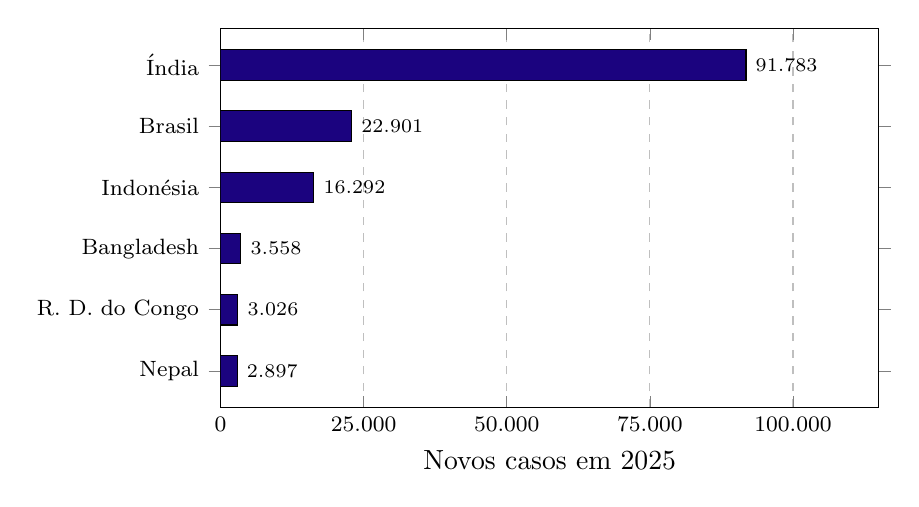
\begin{tikzpicture}
\begin{axis}[
    xbar,
    width=0.82\textwidth,
    height=6.4cm,
    xmin=0, xmax=115000,
    xtick={0,25000,50000,75000,100000},
    xlabel={Novos casos em 2025},
    symbolic y coords={Nepal, {R. D. do Congo}, Bangladesh, Indonésia, Brasil, Índia},
    ytick=data,
    yticklabel style={font=\footnotesize},
    nodes near coords={\pgfmathprintnumber[set thousands separator={.}]{\pgfplotspointmeta}},
    nodes near coords align={horizontal},
    every node near coord/.append style={font=\scriptsize},
    bar width=11pt,
    enlarge y limits=0.12,
    xmajorgrids=true,
    grid style=dashed,
    scaled x ticks=false,
    xticklabel style={font=\footnotesize, /pgf/number format/.cd, set thousands separator={.}, fixed}
]
\addplot[fill=blue!65!black, draw=black] coordinates {
    (2897,Nepal)
    (3026,{R. D. do Congo})
    (3558,Bangladesh)
    (16292,Indonésia)
    (22901,Brasil)
    (91783,Índia)
};
\end{axis}
\end{tikzpicture}
\fonte{Organização Mundial da Saúde, \textit{Global Health Observatory} (indicador WHS3\_45), dados de 2025 \cite{oms2026gho}.}
\end{figure}

A análise automatizada de imagens dermatológicas tem sido investigada
por meio de técnicas de aprendizado de máquina e aprendizado profundo.
\estudo{E01} identificou 21 estudos sobre inteligência
artificial no apoio ao diagnóstico da hanseníase e observou que a
maior parte utilizava imagens de lesões cutâneas e tarefas de
classificação multiclasse. A inclusão da hanseníase em sistemas voltados
a diferentes doenças indica que os resultados dessas propostas devem ser
interpretados tanto em relação ao conjunto de classes quanto ao
reconhecimento específico da doença.

Entre os estudos experimentais, \estudo{E24}
desenvolveu uma abordagem baseada em MobileNetV2 para classificar
imagens de eczema, sarampo, hanseníase e pele saudável, incorporando o
modelo a um protótipo Android. \estudo{E05}, por sua vez,
avaliou ResNet-50 e VGG-16 na classificação de cinco doenças tropicais
negligenciadas com manifestações cutâneas. Em outra linha de
investigação, \estudo{E23} propôs um sistema baseado em YOLOv8
para localizar e classificar lesões de diferentes condições, incluindo
hanseníase, com uso de mapas de saliência para apoiar a interpretação
das predições. Esses trabalhos ilustram abordagens distintas de análise
de imagens, com diferentes requisitos de dados, saídas e procedimentos
de avaliação.

O campo também compreende tarefas relacionadas ao acompanhamento de
manifestações e complicações da doença. \estudo{E21}
apresentou o CO2Wounds-V2, um conjunto de fotografias de feridas
crônicas de pacientes com hanseníase, acompanhado de experimentos de
segmentação semântica. Nesse caso, a tarefa consiste em delimitar
regiões de ferida nas imagens, e não em determinar se o paciente
apresenta hanseníase. Essa distinção é necessária para organizar a
literatura e evitar que medidas de segmentação sejam interpretadas como
evidências de desempenho diagnóstico.

A caracterização das populações representadas nos dados também integra a
avaliação dos modelos. \estudo{E05} utilizou fotografias
coletadas em Costa do Marfim e Gana, descrevendo a população como
composta por pessoas de pele escura, com fototipos de Fitzpatrick IV ou
superiores. O estudo oferece evidências diretamente relacionadas à
análise de imagens de pele escura, mas não apresenta comparação de
desempenho entre os diferentes fototipos. \estudo{E23} também
reconhece limitações na diversidade dos dados e aponta a ampliação da
representação de pessoas com tons de pele mais escuros como uma direção
de trabalho futuro.

Esses estudos motivam a investigação de como o desempenho dos modelos é
definido, mensurado e interpretado. Para o presente trabalho, a
avaliação compreende os resultados preditivos relativos à tarefa, os
procedimentos empregados para obtê-los e as evidências disponíveis sobre
sua aplicação a novos dados e a diferentes grupos de tom de pele. A
utilização futura em apoio à triagem na rede pública de saúde do Brasil
constitui o contexto de interesse da pesquisa, sem que os resultados
computacionais sejam, por si só, considerados demonstração de
efetividade clínica.

\section{Problema}\label{problema}

A existência de modelos capazes de reconhecer padrões em imagens não
estabelece, isoladamente, sua adequação à identificação de manifestações
de hanseníase em uma população específica. Os estudos analisados
apresentam diferenças nas tarefas, nas classes de interesse, na
composição dos conjuntos de dados e nas métricas utilizadas. Classificar
uma imagem entre doenças, localizar uma lesão e segmentar uma ferida
produzem resultados com significados distintos. Consequentemente, uma
comparação baseada apenas nos maiores valores publicados pode
desconsiderar diferenças essenciais entre os experimentos \estudo{E05,E21,E23}.

Além disso, medidas agregadas podem não representar adequadamente o
desempenho referente à hanseníase. No estudo de \estudo{E05}, a
Task 2 apresentou acurácias globais de 77\% e 80\% nos dois cenários
avaliados. Entretanto, a leitura da diagonal correspondente à hanseníase
nas matrizes de confusão indica proporções de classificação correta de
12\% e 13\%, respectivamente. Como as linhas representam a classe real,
esses valores podem ser interpretados como sensibilidade por imagem para
a classe hanseníase. O contraste evidencia a importância de examinar
resultados específicos por doença, em vez de atribuir à hanseníase o
desempenho global do sistema.

A relação entre os resultados obtidos e os tons de pele constitui outra
dimensão do problema. A presença de imagens de pele escura em um
conjunto de dados não demonstra que o modelo apresente comportamento
equivalente entre diferentes tons. No estudo de \estudo{E05}, a
população é caracterizada por um intervalo de fototipos, mas não são
fornecidos resultados separados por esses grupos. Já \estudo{E23}
reconhece limitações de representatividade e a necessidade de ampliar a
diversidade dos dados. Essas observações sustentam a necessidade de
examinar a caracterização populacional e a avaliação por grupos, sem
permitir concluir, a partir dessas evidências isoladas, que todos os
modelos tenham desempenho inferior em pele negra.

Também permanece necessário distinguir a avaliação computacional da
avaliação em contexto assistencial. O desenvolvimento de um aplicativo
ou a obtenção de resultados em conjuntos de imagens não comprova sua
contribuição para o atendimento em serviços de saúde. Enquanto
\estudo{E24} apresenta um protótipo de
aplicação móvel, \estudo{E23} situa os estudos prospectivos com
dermatologistas entre as atividades futuras. Assim, a relevância dessas
propostas para a rede pública exige considerar o alcance e os limites
dos procedimentos de validação relatados.

Diante desse cenário, o problema investigado consiste em compreender
quais evidências e procedimentos permitem avaliar o desempenho de
modelos de visão computacional na identificação de manifestações
dermatológicas associadas à hanseníase, no contexto de apoio à triagem
na rede pública de saúde do Brasil, considerando a tarefa realizada, as
características dos dados e os limites de generalização dos resultados.
A comparação entre tons de pele será examinada quando houver informações
disponíveis, como uma dimensão complementar da avaliação. A revisão em
andamento buscará sistematizar essas informações e identificar os
aspectos que precisam ser considerados no planejamento de avaliações
futuras.

\section{Questão de pesquisa}\label{gqm-adaptado-e-questuxe3o-de-pesquisa}

\subsection{GQM adaptado}

O objetivo de análise foi organizado por meio de um GQM adaptado, que
explicita o objeto, o propósito, o foco, o ponto de vista e o contexto
da investigação. O quadro orienta a definição da questão de pesquisa e
das medidas a serem extraídas dos estudos.

{\def\LTcaptype{none} % do not increment counter
\begin{longtable}[]{@{}
  >{\raggedright\arraybackslash}p{(\linewidth - 2\tabcolsep) * \real{0.5000}}
  >{\raggedright\arraybackslash}p{(\linewidth - 2\tabcolsep) * \real{0.5000}}@{}}
\toprule\noalign{}
\begin{minipage}[b]{\linewidth}\raggedright
Característica
\end{minipage} & \begin{minipage}[b]{\linewidth}\raggedright
Valor
\end{minipage} \\
\midrule\noalign{}
\endhead
\bottomrule\noalign{}
\endlastfoot
\textbf{Analisar} & Modelos de visão computacional aplicados à
identificação de manifestações dermatológicas. \\
\textbf{Com o propósito de} & Avaliar o desempenho dos modelos aplicados
à identificação de padrões em imagens de pele. \\
\textbf{Com foco em} & Identificação de características patológicas de
hanseníase. \\
\textbf{Do ponto de vista de} & Pesquisadores das áreas de Engenharia de
Software e da área da saúde. \\
\textbf{No contexto de} & Apoio à triagem de hanseníase na rede pública
de saúde do Brasil. \\
\end{longtable}
}

\subsection{Questão norteadora}

A investigação é orientada pela seguinte questão:

\begin{quote}
Como avaliar o desempenho de modelos de visão computacional aplicados à
identificação de padrões associados à hanseníase em imagens de pele, no
contexto da rede pública de saúde do Brasil?
\end{quote}

Nesta etapa, a questão será abordada por meio da identificação e análise
das evidências apresentadas na literatura. Serão examinadas as tarefas
realizadas, os modelos empregados, as características dos conjuntos de
dados, os procedimentos de avaliação, as métricas e os resultados, bem
como as informações disponíveis sobre tons de pele e generalização. A
ausência de avaliação por grupo será registrada como uma limitação das
evidências disponíveis, sem ser tomada como demonstração de equidade ou
de desigualdade de desempenho.

\section{Objetivos}\label{objetivos}

\subsection{Objetivo geral}\label{objetivo-geral}

Analisar a avaliação de desempenho de modelos de visão computacional
aplicados à identificação de padrões associados à hanseníase em imagens
de pele, a partir da síntese das evidências da literatura, visando
fundamentar seu uso em apoio à triagem na rede pública de saúde do
Brasil.

\subsection{Objetivos específicos}\label{objetivos-especuxedficos}

\begin{enumerate}
\def\labelenumi{\arabic{enumi}.}
\tightlist
\item
  Caracterizar as tarefas, os modelos e as abordagens de visão
  computacional empregados na análise de manifestações dermatológicas
  associadas à hanseníase.
\item
  Identificar os conjuntos de dados utilizados, suas formas de aquisição
  e anotação e as informações disponíveis sobre as populações e os tons
  de pele representados.
\item
  Sistematizar os procedimentos de avaliação, as métricas e os
  resultados reportados, distinguindo medidas globais, resultados
  específicos de hanseníase e unidades de análise.
\item
  Examinar as evidências de generalização e de avaliação do desempenho
  entre grupos de tom de pele, quando disponíveis.
\item
  Identificar limitações e lacunas que fundamentem o planejamento de uma
  avaliação futura de modelos no contexto de apoio à triagem na rede
  pública de saúde do Brasil.
\end{enumerate}


\section{Metodologia}

Este trabalho adota uma revisão estruturada da literatura para identificar e
analisar evidências sobre a avaliação de modelos de visão computacional
aplicados à identificação de padrões associados à hanseníase em imagens de
pele. A Figura~\ref{fig:percurso-metodologico} apresenta o percurso da
revisão, do problema de pesquisa à síntese das evidências.

\begin{figure}[htbp]
\centering
\small
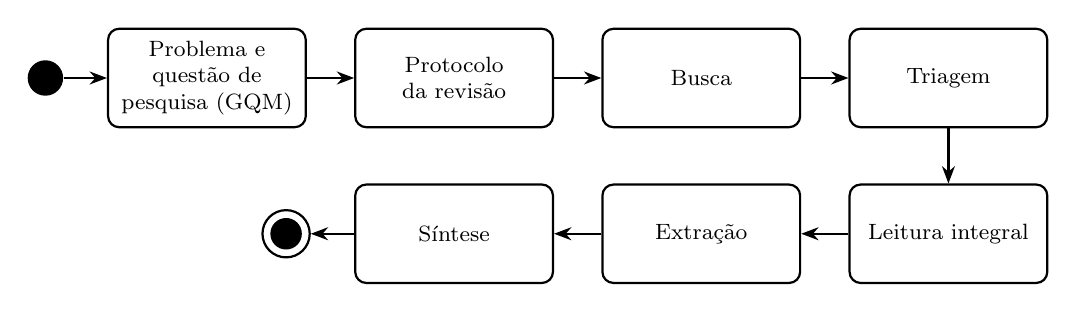
\begin{tikzpicture}[
  node distance=0.7cm and 0.6cm,
  etapa/.style={draw=black, thick, rounded corners=4pt, fill=white,
    text width=2.3cm, minimum height=1.25cm, align=center, font=\footnotesize, inner sep=3pt},
  inicio/.style={circle, fill=black, minimum size=0.45cm, inner sep=0pt},
  seta/.style={-{Stealth[length=2.2mm]}, thick}
]
\node[inicio] (ini) {};
\node[etapa, right=0.55cm of ini] (a1) {Problema e questão de pesquisa (GQM)};
\node[etapa, right=of a1] (a2) {Protocolo da revisão};
\node[etapa, right=of a2] (a3) {Busca};
\node[etapa, right=of a3] (a4) {Triagem};
\node[etapa, below=of a4] (b5) {Leitura integral};
\node[etapa, left=of b5] (b6) {Extração};
\node[etapa, left=of b6] (b7) {Síntese};
\node[circle, draw=black, thick, minimum size=0.6cm, inner sep=0pt, left=0.55cm of b7] (fim) {};
\fill (fim.center) circle (0.2cm);
\draw[seta] (ini) -- (a1);
\draw[seta] (a1) -- (a2);
\draw[seta] (a2) -- (a3);
\draw[seta] (a3) -- (a4);
\draw[seta] (a4) -- (b5);
\draw[seta] (b5) -- (b6);
\draw[seta] (b6) -- (b7);
\draw[seta] (b7) -- (fim);
\end{tikzpicture}
\caption{Fluxo de atividades da revisão estruturada da literatura}
\label{fig:percurso-metodologico}
\fonte{Elaboração própria.}
\end{figure}

\subsection{Classificação do estudo}

A classificação segue as dimensões do Capítulo~2 de \citeonline{wohlin2024}.

\begin{itemize}
\item \textbf{Finalidade descritiva} \cite[p.~11--13]{wohlin2024}. A pesquisa
descritiva descreve um fenômeno ou as características de um problema, e sua
questão costuma começar com ``o quê'' ou ``como'' \cite[p.~12]{wohlin2024}.
A questão norteadora começa com ``Como'', e os objetivos específicos 1 a 4
pedem caracterizar, identificar, sistematizar e examinar o que os estudos
reportam.

\item \textbf{Abordagem mista} \cite[p.~13]{wohlin2024}. A extração reúne
dados quantitativos (como número de imagens e métricas) e qualitativos (como
tarefa, modelo e população). O Capítulo~\ref{cap:revisao-literatura} combina
contagens e tabelas com síntese descritiva.

\item \textbf{Coleta por estudo de literatura estruturado}
\cite[p.~16--17]{wohlin2024}. A revisão tem questões de pesquisa, protocolo,
estratégia de busca, critérios explícitos de seleção e formulário de extração,
características que \citeonline[p.~4]{kitchenham2007} apontam como diferenciais
da revisão sistemática em relação à revisão convencional.

\item \textbf{Análise descritiva e por classificação}
\cite[p.~18]{wohlin2024}. Os estudos são resumidos por contagens e tabelas e
classificados por tarefa, modelo e procedimento de avaliação.
\end{itemize}

\subsection{Etapas e atividades da revisão}

A Tabela~\ref{tab:etapas-metodologia} lista as atividades realizadas na revisão
e indica onde cada uma é apresentada.

\begin{table}[htb]
\centering
\caption{Atividades realizadas na revisão estruturada}
\label{tab:etapas-metodologia}
\footnotesize
\begin{tabular}{>{\raggedright\arraybackslash}p{3.0cm} >{\raggedright\arraybackslash}p{5.6cm} >{\raggedright\arraybackslash}p{6.0cm}}
\toprule
\textbf{Atividade} & \textbf{Descrição} & \textbf{Onde está} \\
\midrule
Problema e questão de pesquisa & Definição do problema, da questão norteadora (GQM adaptado) e dos objetivos & Capítulo~1 \\
Protocolo da revisão & Questões de pesquisa, estratégia de busca (PICOC), critérios de seleção e formulário de extração & Capítulo~\ref{cap:revisao-literatura}, seções ``Planejamento e protocolo'' e ``Estruturação da estratégia de busca''; subseções ``Critérios de seleção'' e ``Extração e síntese das evidências''; Figura~\ref{fig:fluxo-metodologico-ia} \\
Busca & Execução da busca e identificação dos registros & Capítulo~\ref{cap:revisao-literatura}, seção ``Realização da busca e seleção dos artigos'' \\
Triagem & Seleção por título e resumo, com os critérios do protocolo & Mesma seção; Figura~\ref{fig:fluxo-triagem} \\
Leitura integral & Leitura dos textos completos e confirmação da elegibilidade & Mesma seção \\
Extração & Preenchimento do formulário de extração dos estudos incluídos & Subseção ``Extração e síntese das evidências'' \\
Síntese & Síntese das evidências por questão de pesquisa & Seção ``Resultados da revisão'' \\
\bottomrule
\end{tabular}
\fonte{Elaboração própria.}
\end{table}

\subsection{Evidências da revisão e elementos do escopo e do planejamento}

As evidências reunidas na revisão estruturada (Capítulo~\ref{cap:revisao-literatura})
organizam-se em consonância com as etapas de definição do escopo (\textit{Scoping}, Capítulo~8)
e de planejamento (\textit{Planning}, Capítulo~9) do processo experimental de \citeonline{wohlin2024},
apresentado no Capítulo~\ref{cap:referencial-teorico} (Figura~\ref{fig:processo-experimento}):

\begin{itemize}
\item \textbf{Definição do escopo (\textit{Scoping}, Capítulo~8)} \cite[p.~109--114]{wohlin2024}:
o escopo é formalizado por um modelo de objetivo estruturado em cinco elementos fundamentais:
objeto de estudo, propósito, foco de qualidade, perspectiva e contexto \cite[p.~109--110]{wohlin2024}.
No presente trabalho, o modelo GQM adaptado (Quadro da Seção~\ref{gqm-adaptado-e-questuxe3o-de-pesquisa})
cumpre essa função, delimitando os modelos de visão computacional (objeto) voltados a avaliar o desempenho
diagnóstico (propósito), focando a identificação de manifestações da hanseníase (foco), sob a perspectiva
de pesquisadores e da atenção à saúde, no contexto da triagem na rede pública do Brasil.

\item \textbf{Planejamento experimental (\textit{Planning}, Capítulo~9)} \cite[p.~115--144]{wohlin2024}:
o planejamento operacionaliza o escopo em sete dimensões: seleção do contexto (Seção~9.1),
formulação de hipóteses (Seção~9.2), seleção de variáveis dependentes e independentes (Seção~9.3),
seleção de sujeitos e populações (Seção~9.4), desenho experimental (Seção~9.5), instrumentação
(Seção~9.6) e avaliação de ameaças à validade (Seções~9.7 e 9.8).
\end{itemize}

A Tabela~\ref{tab:planejamento-wohlin} relaciona cada um desses elementos ao que a revisão
reúne e aos limites das evidências identificadas na literatura. A correspondência dá-se por analogia:
os sujeitos descritos por Wohlin correspondem aqui aos conjuntos de dados e às amostras demográficas de imagens
clínicas de lesões, enquanto os objetos experimentais correspondem aos modelos e algoritmos de visão
computacional sob avaliação.

\begin{table}[htb]
\centering
\caption{Elementos do escopo e do planejamento experimental e evidências da revisão}
\label{tab:planejamento-wohlin}
\footnotesize
\begin{tabular}{>{\raggedright\arraybackslash}p{3.6cm} >{\raggedright\arraybackslash}p{4.3cm} >{\raggedright\arraybackslash}p{6.5cm}}
\toprule
\textbf{Elemento (seção; página)} & \textbf{O que a revisão reúne} & \textbf{Limite das evidências} \\
\midrule
Escopo (8.1; p.~109--110) & GQM adaptado: objeto, propósito, foco, perspectiva e contexto & ``Foco'' e ``contexto'' descrevem domínio e cenário de uso \\
Contexto e sujeitos (9.1 e 9.4; p.~115 e 118) & Contexto do GQM (rede pública de saúde do Brasil); conjuntos de dados e populações usados nos estudos & Poucos estudos caracterizam o tom de pele da base \\
Variáveis (9.3; p.~118) & Modelos e abordagens identificados; métricas e procedimentos reportados & Em dois estudos, o desempenho para a hanseníase é bem inferior ao indicador global ou ao Top-5 (Subseção~\ref{subsec:rq4-metricas}) \\
Desenho (9.5; p.~119) & Procedimentos de avaliação dos estudos (divisão dos dados e validação) & A maior parte dos estudos que desenvolvem modelos não informa a unidade da divisão dos dados, e poucos testam em outra base (Subseção~\ref{subsec:rq3-metodos}) \\
Validade (9.7 e 9.8; p.~128 a 138) & Lacunas da evidência (separação por paciente, generalização e tom de pele) & Nenhum estudo com dados reporta, no texto principal, desempenho por tom de pele (Subseção~\ref{subsec:rq5-rq6-tom-pele}) \\
\bottomrule
\end{tabular}
\fonte{Elaboração própria, com os elementos dos capítulos 8 e 9 de \citeonline{wohlin2024}.}
\end{table}

\section{Organização do trabalho}

Este trabalho está organizado em três capítulos. O primeiro apresenta o
contexto, o problema de pesquisa, a questão norteadora, os objetivos e a
metodologia. O segundo reúne os fundamentos sobre pesquisa empírica,
hanseníase, visão computacional e avaliação de modelos. O terceiro apresenta a
revisão estruturada da literatura: o planejamento e o protocolo, a estratégia
de busca, a seleção dos estudos, a extração e a síntese das evidências e os
resultados, organizados pelas questões de pesquisa. Ao final, são apresentadas
as referências e os apêndices.

\section{Cronograma e fluxo de atividades}

Esta seção apresenta as atividades realizadas, em forma de fluxo na
Figura~\ref{fig:percurso-metodologico}.

\begin{itemize}
\item \textbf{Definição do problema, da questão de pesquisa e dos objetivos:}
formulação do problema e da questão norteadora, com o GQM adaptado, e dos
objetivos geral e específicos.
\item \textbf{Elaboração do protocolo da revisão:} definição das questões de
pesquisa, da estratégia de busca (PICOC), dos critérios de inclusão e exclusão
e do formulário de extração.
\item \textbf{Busca dos registros:} execução da busca e identificação dos
registros.
\item \textbf{Triagem:} seleção por título e resumo, com os critérios do
protocolo.
\item \textbf{Leitura integral:} leitura dos textos completos e confirmação da
elegibilidade.
\item \textbf{Extração:} preenchimento do formulário de extração dos estudos
incluídos.
\item \textbf{Síntese:} síntese das evidências por questão de pesquisa.
\end{itemize}

O fluxo de seleção e os resultados são apresentados no
Capítulo~\ref{cap:revisao-literatura}.

% !TeX root = ../tcc.tex
\chapter{Referencial teórico}
\label{cap:referencial-teorico}

Neste capítulo são apresentados os conceitos que fundamentam a investigação.
Inicialmente, são abordadas a pesquisa empírica em engenharia de software
e a revisão sistemática da literatura. Em seguida, são apresentados aspectos
da hanseníase, da aplicação de aprendizado de máquina a imagens de pele e
das medidas usadas na avaliação dos modelos.

\section{Experimentação na engenharia de software}

A pesquisa empírica utiliza observações e dados para investigar fenômenos,
avaliar propostas e fundamentar conclusões. Na engenharia de software, as
estratégias empíricas incluem experimentos, estudos de caso e estudos
secundários de literatura, cada qual com objetivos e procedimentos próprios
\cite{wohlin2024}. A escolha entre essas estratégias depende da questão
investigada e das evidências necessárias para respondê-la.

Um experimento controlado envolve a definição de fatores, tratamentos e
medidas para investigar seus efeitos sob condições estabelecidas. Já uma
revisão sistemática é um estudo secundário, no qual as evidências de outros
trabalhos são identificadas e analisadas a partir de um processo documentado
\cite[p. 51--56]{wohlin2024}. Neste TCC, a revisão busca reunir informações
sobre avaliações de modelos; sua realização não constitui, por si só, um
experimento controlado ou uma validação clínica.

\subsection{Experimento}

Um experimento é empregado para investigar questões por meio de observações
sob condições planejadas. Sua definição envolve, entre outros elementos, o
objeto estudado, os tratamentos ou fatores considerados e as medidas usadas
para observar seus efeitos. A organização do processo contribui para que
as condições da investigação e os limites de interpretação sejam
explicitados \cite[p. 79--82]{wohlin2024}. Esses conceitos são apresentados
como fundamentação para o trabalho e não indicam que um experimento já
foi executado.

A Figura~\ref{fig:processo-experimento} apresenta uma visão geral do
processo experimental proposto por \citeonline{wohlin2024}: definição do
escopo, planejamento, operação, análise e interpretação, e apresentação
e documentação. A figura ilustra o referencial metodológico; ela não
representa um experimento já executado neste TCC.

\begin{figure}[htbp]
\centering
\caption{Visão geral do processo experimental}
\label{fig:processo-experimento}
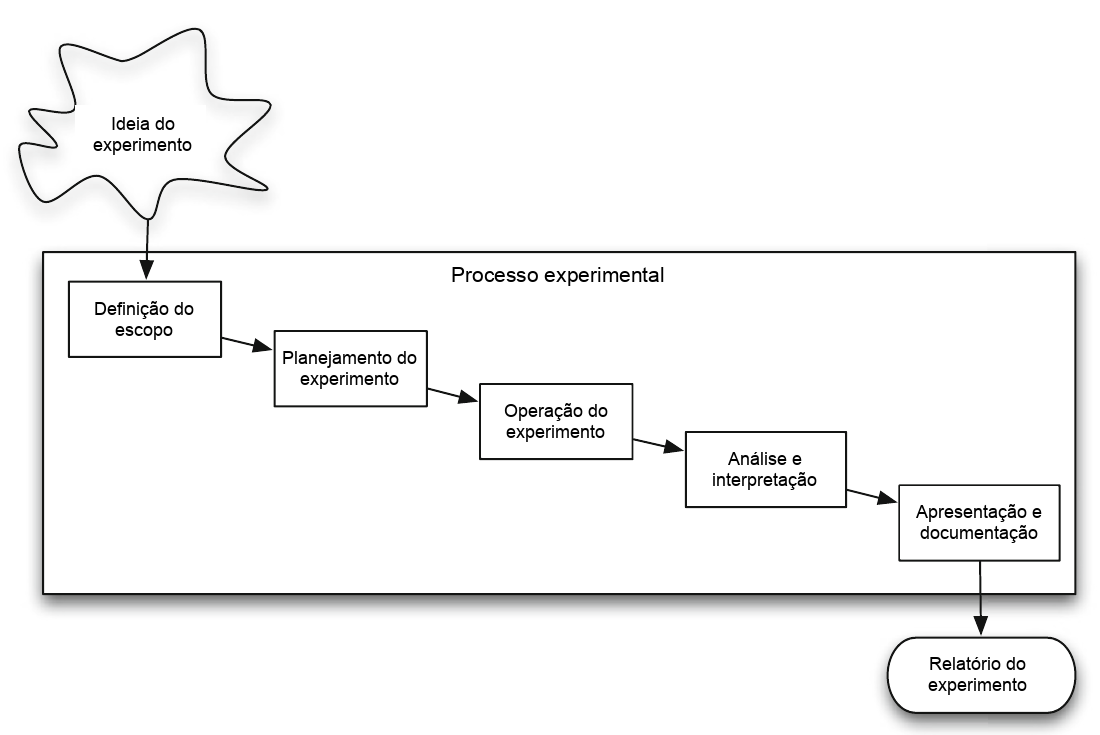
\includegraphics[width=0.88\textwidth]{figuras/processo-experimental-wohlin-2024.png}
\fonte{Adaptado de \citeonline{wohlin2024}.}
\end{figure}

\subsubsection{Definição do escopo}

A definição do escopo delimita o objeto, o propósito, o foco de qualidade,
a perspectiva e o contexto do estudo. Esses elementos orientam a pergunta
que se pretende responder e as decisões das etapas seguintes. O GQM
adaptado apresentado na introdução \cite{basili1994} explicita esses componentes para o
objetivo desta pesquisa \cite[p. 80]{wohlin2024}.

\subsubsection{Planejamento}

No planejamento são especificados o contexto da investigação, as variáveis,
as hipóteses quando aplicáveis, o desenho e os instrumentos de medição.
Também são examinadas possíveis ameaças à validade. Em uma avaliação de
modelos de visão computacional, essas decisões poderiam envolver a
caracterização dos dados, a definição das tarefas e a escolha das métricas;
o desenho efetivo de uma avaliação futura ainda depende dos resultados da
revisão \cite[p. 80--82]{wohlin2024}.

\subsubsection{Operação}

A operação corresponde à preparação e à execução do procedimento
planejado, incluindo a coleta e a verificação dos dados produzidos. Seu
registro permite relacionar os resultados às condições em que foram
obtidos. Nesta etapa do TCC, a operação de um experimento com modelos não
foi estabelecida \cite{wohlin2024}.

\subsubsection{Análise e interpretação}

Após a obtenção dos dados, a análise organiza as medidas e examina os
resultados em relação às questões formuladas. A interpretação deve
considerar as características dos dados e as ameaças à validade, evitando
estender conclusões além das condições de avaliação \cite{wohlin2024}.

\subsubsection{Apresentação e documentação}

O relato reúne o objetivo, o procedimento, as medidas, os resultados e as
limitações, permitindo que outras pessoas compreendam e examinem o estudo.
A documentação também dá suporte à comparação com investigações posteriores
\cite{wohlin2024}.

\subsection{Revisão sistemática da literatura}

Uma revisão sistemática parte de questões de pesquisa e de um protocolo
que orienta a busca, a seleção, a avaliação e a síntese dos estudos. Entre
os elementos a registrar estão as fontes e estratégias de busca, os critérios
de seleção e os procedimentos de extração de dados
\cite{kitchenham2007,wohlin2024}. A descrição dessas decisões permite
examinar o alcance e as limitações do conjunto de estudos identificado.

No presente trabalho, a revisão é empregada para compreender como modelos
aplicados a imagens de pele relacionadas à hanseníase são avaliados. O
protocolo e o andamento de sua execução são apresentados no
Capítulo~\ref{cap:revisao-literatura}.

\section{Hanseníase e identificação de manifestações cutâneas}

A hanseníase pode apresentar manifestações na pele e comprometimento de
nervos periféricos. Segundo a \citeonline{oms2018hanseniase}, entre os
sinais usados para o diagnóstico estão a perda de sensibilidade em uma
mancha cutânea, alterações em nervos periféricos associadas à perda de
sensibilidade e a presença de bacilos em exame de esfregaço cutâneo.
Portanto, uma fotografia de pele representa somente parte das informações
consideradas na avaliação clínica.

No contexto desta pesquisa, a análise computacional de imagens é tratada
como possível apoio à triagem. Seu desempenho em uma base de imagens não
demonstra, isoladamente, que o sistema possa estabelecer um diagnóstico ou
melhorar o atendimento em um serviço de saúde. Por isso, é necessário
relacionar os resultados reportados à tarefa realizada, aos dados utilizados
e à forma de validação \estudo{E01}.

\section{Inteligência artificial e visão computacional}

\subsection{Aprendizado de máquina e aprendizado profundo}

A visão computacional compreende métodos capazes de extrair e analisar
informações de imagens. No aprendizado de máquina, modelos são ajustados a
partir de dados para executar uma tarefa; no aprendizado profundo, redes com
múltiplas camadas aprendem representações em diferentes níveis. Redes
neurais convolucionais são uma das abordagens empregadas na análise de
imagens \cite{lecun2015deep}.

\subsection{Tarefas de análise de imagens}

As aplicações à hanseníase diferem quanto à tarefa e ao resultado produzido.
Na classificação, o modelo atribui uma categoria à imagem; na detecção,
identifica e localiza objetos ou lesões; na segmentação, associa regiões ou
pixels a classes de interesse. Essas saídas respondem a perguntas diferentes
e devem ser avaliadas com medidas apropriadas à tarefa
\estudo{E05,E21,E23}.

Por exemplo, \estudo{E05} investigou a classificação de doenças
tropicais com manifestações cutâneas, enquanto \estudo{E21}
estudou a segmentação de feridas em imagens de pessoas com hanseníase.
Delimitar uma ferida e identificar a doença em uma imagem são objetivos
distintos; assim, um resultado de segmentação não deve ser apresentado como
medida de diagnóstico da hanseníase.

\section{Métricas e dimensões de avaliação}\label{muxe9tricas-e-dimensuxf5es-de-avaliauxe7uxe3o-do-gqm}

As métricas serão extraídas conforme a tarefa e o protocolo de cada
estudo. Não se exige que todos os artigos apresentem todas as medidas.
Métricas ausentes serão registradas como não reportadas; cálculos
adicionais somente serão realizados quando houver dados suficientes, com
identificação explícita de que foram derivados nesta revisão.

\subsection{Resultados de
classificação}\label{resultados-de-classificauxe7uxe3o}

Para classificação binária, deve-se definir previamente o que constitui
a classe positiva e o diagnóstico/rótulo de referência. Em modelos
multiclasse, a hanseníase pode ser analisada como classe positiva frente
às demais classes (um contra todos). As definições abaixo se referem à
unidade avaliada --- por exemplo, imagem --- e não implicam
automaticamente diagnóstico por paciente.

{\def\LTcaptype{none} % do not increment counter
\begin{longtable}[]{@{}
  >{\raggedright\arraybackslash}p{(\linewidth - 2\tabcolsep) * \real{0.5000}}
  >{\raggedright\arraybackslash}p{(\linewidth - 2\tabcolsep) * \real{0.5000}}@{}}
\toprule\noalign{}
\begin{minipage}[b]{\linewidth}\raggedright
Resultado
\end{minipage} & \begin{minipage}[b]{\linewidth}\raggedright
Significado
\end{minipage} \\
\midrule\noalign{}
\endhead
\bottomrule\noalign{}
\endlastfoot
\textbf{TP --- True Positive} & A unidade pertence à classe positiva
segundo a referência e o modelo a classifica como positiva. \\
\textbf{TN --- True Negative} & A unidade pertence à classe negativa
segundo a referência e o modelo a classifica como negativa. \\
\textbf{FP --- False Positive} & A unidade pertence à classe negativa
segundo a referência, mas o modelo a classifica como positiva. \\
\textbf{FN --- False Negative} & A unidade pertence à classe positiva
segundo a referência, mas o modelo a classifica como negativa. \\
\end{longtable}
}

A classe positiva pode representar hanseníase ou uma manifestação
definida no protocolo do estudo. Essas tarefas devem ser distinguidas:
reconhecer uma ferida em paciente com hanseníase não equivale a
diagnosticar a doença.

\subsection{Métricas relacionadas à questão de
pesquisa}\label{muxe9tricas-relacionadas-uxe0-questuxe3o-de-pesquisa}

{\def\LTcaptype{none} % do not increment counter
\begin{longtable}[]{@{}
  >{\raggedright\arraybackslash}p{(\linewidth - 6\tabcolsep) * \real{0.2500}}
  >{\raggedright\arraybackslash}p{(\linewidth - 6\tabcolsep) * \real{0.2500}}
  >{\raggedright\arraybackslash}p{(\linewidth - 6\tabcolsep) * \real{0.2500}}
  >{\raggedright\arraybackslash}p{(\linewidth - 6\tabcolsep) * \real{0.2500}}@{}}
\toprule\noalign{}
\begin{minipage}[b]{\linewidth}\raggedright
ID
\end{minipage} & \begin{minipage}[b]{\linewidth}\raggedright
Dimensão do desempenho
\end{minipage} & \begin{minipage}[b]{\linewidth}\raggedright
Métrica
\end{minipage} & \begin{minipage}[b]{\linewidth}\raggedright
Descrição e operacionalização
\end{minipage} \\
\midrule\noalign{}
\endhead
\bottomrule\noalign{}
\endlastfoot
M1 & Classificação & \textbf{Sensibilidade --- Sensitivity (SEN/Recall)}
& Proporção de positivos corretamente identificados: \textbf{SEN = TP /
(TP + FN)}. \\
M2 & Classificação & \textbf{Especificidade --- Specificity (SPE)} &
Proporção de negativos corretamente identificados: \textbf{SPE = TN /
(TN + FP)}. \\
M3 & Classificação & \textbf{Precisão --- Precision (PRE)} & Proporção
de predições positivas que correspondem a positivos de referência:
\textbf{PRE = TP / (TP + FP)}. \\
M4 & Classificação & \textbf{F1-score} & Média harmônica entre precisão
e sensibilidade, considerando o efeito de falsos positivos e falsos
negativos: \textbf{F1 = 2 $\times$ PRE $\times$ SEN / (PRE + SEN)}, ou \textbf{2TP /
(2TP + FP + FN)}. \\
M5 & Classificação geral & \textbf{Acurácia --- Accuracy (ACC)} &
Proporção total de classificações corretas: \textbf{ACC = (TP + TN) /
(TP + TN + FP + FN)}, na formulação binária. Para multiclasse, usar
acertos totais / unidades totais. \\
M6 & Equidade do desempenho & \textbf{Diferença de desempenho entre
grupos} & Comparação da mesma métrica entre grupos de tons de pele,
quando disponível. Para dois grupos A e B: \textbf{$\Delta$ = métrica(A) $-$
métrica(B)}, com grupos e direção identificados. Registrar tamanhos dos
grupos, condições de avaliação e incerteza, quando reportados. \\
M7 & Generalização & \textbf{Variação de desempenho entre datasets} &
Comparação da mesma métrica entre avaliações em dados de distribuição
semelhante à de treinamento e dados de distribuição diferente:
\textbf{gap = métrica(ID) $-$ métrica(OOD)}, quando o desenho permitir.
Registrar se houve adaptação ou retreinamento e se tarefa/classes são
comparáveis. \\
M8 & Segmentação / sobreposição espacial & \textbf{Intersection over
Union (IoU)} & Interseção dividida pela união das regiões prevista P e
de referência G: \textbf{IoU = área(P $\cap$ G) / área(P $\cup$ G)}. Em máscaras
binárias: \textbf{IoU = TP\_pixel / (TP\_pixel + FP\_pixel +
FN\_pixel)}. Registrar mIoU separadamente quando houver média entre
classes. \\
M9 & Detecção / segmentação por instância & \textbf{Mean Average
Precision (mAP)} & Média dos valores de AP das classes consideradas; AP
resume a curva precisão--recall segundo a convenção do benchmark.
Registrar o critério de correspondência e o limiar de IoU: por exemplo,
\textbf{mAP@0,50} ou \textbf{mAP@0,50:0,95}. Distinguir AP de caixas e
AP de máscaras. \\
\end{longtable}
}

\textbf{IoU e mAP não são métricas exclusivas de segmentação.} Em
detecção, IoU mede sobreposição de caixas e pode determinar a
correspondência entre predição e referência; mAP resume o desempenho das
detecções. Na segmentação semântica, IoU/mIoU mede sobreposição de
máscaras por classe. Na segmentação por instância, também se utiliza
AP/mAP calculada sobre máscaras. A documentação de avaliação COCO
explicita essa distinção entre caixas e máscaras \cite{coco}.

\textbf{Critérios de interpretação:} registrar se a unidade é paciente,
imagem, objeto ou pixel; separar resultados específicos de hanseníase de
médias globais; identificar médias macro, micro ou ponderadas; registrar
denominadores nulos como indefinidos ou conforme a convenção explicitada
no estudo. Diferenças entre métricas expressas em porcentagem devem ser
apresentadas em pontos percentuais. M6 e M7 são dimensões de comparação,
não métricas únicas universalmente definidas. Desempenhos de modelos
diferentes em bases diferentes não isolam o efeito da mudança de
distribuição.

O conjunto de métricas funciona como orientação para extração, não como
lista fechada. Medidas adicionais reportadas pelos artigos, como MCC,
devem ser registradas com sua definição e contexto. A análise de
equidade não será restrição de elegibilidade dos artigos e não será
presumida quando não houver resultados por grupo.


\section{Avaliação e generalização dos modelos}

A avaliação de um modelo depende do desenho do estudo e da relação entre
os dados usados no desenvolvimento e aqueles usados na avaliação. Além do
valor de uma métrica, é necessário identificar o conjunto avaliado, a unidade
de análise e as classes consideradas. Em uma aplicação multiclasse, por
exemplo, uma medida global não descreve necessariamente o desempenho para
cada doença \estudo{E05}.

A generalização diz respeito ao comportamento do modelo em dados diferentes
dos utilizados no seu desenvolvimento. Evidências obtidas em uma população
ou conjunto específico devem ser interpretadas considerando suas condições
de aquisição e composição. Para a análise por tons de pele, é necessário
verificar se as características dos grupos são descritas e se as medidas
são apresentadas separadamente; a simples presença de um grupo nas imagens
não demonstra desempenho equivalente entre grupos \estudo{E05,E23}.
Esses aspectos orientam a extração das evidências na revisão.

% !TeX root = ../tcc.tex
\chapter{Revisão estruturada da literatura}
\label{cap:revisao-literatura}
\label{sec:conducao-revisao}

A revisão de literatura foi planejada para identificar e analisar evidências
sobre a avaliação de modelos de visão computacional aplicados a manifestações
cutâneas associadas à hanseníase. A definição de uma questão, de um protocolo,
de critérios de seleção e de procedimentos de extração e síntese é coerente
com as orientações de \citeonline{kitchenham2007} para revisões sistemáticas
em engenharia de software. O capítulo 4 de \citeonline{wohlin2024} apresenta a revisão
sistemática como estudo secundário e organiza seu processo em planejamento,
condução e relato. A obra fundamenta a definição de questões e critérios,
a documentação da busca, a seleção e a extração orientada pelas questões
de pesquisa. O procedimento
adotado nesta revisão é descrito a seguir; suas etapas não devem ser
interpretadas como a execução de um experimento controlado.

\section{Planejamento e protocolo}

O objetivo, o protocolo e os critérios foram organizados no Evidentia. A
questão principal é: como avaliar o desempenho de modelos de visão
computacional aplicados à identificação de padrões associados à hanseníase
em imagens de pele, no contexto da rede pública de saúde do Brasil?

As questões secundárias desdobram a questão principal em aspectos necessários
à avaliação dos modelos: técnicas e abordagens utilizadas, dados e populações,
procedimentos, métricas, desempenho entre grupos e generalização. A
identificação dos veículos de publicação complementa a caracterização dos
estudos. Conforme \citeonline{kitchenham2007}, as questões de pesquisa
orientam a definição dos dados a serem extraídos e sintetizados na revisão. A
investigação foi detalhada nas seguintes questões secundárias:

\begin{enumerate}
	\item Quais técnicas de visão computacional são usadas para identificar manifestações dermatológicas associadas à hanseníase?
	\item Quais conjuntos de dados e populações são utilizados no desenvolvimento e na avaliação dos modelos?
	\item Quais métodos e procedimentos são usados para avaliar o desempenho e quais resultados são relatados?
	\item Quais métricas são usadas na avaliação e quais resultados são relatados?
	\item Como o desempenho varia entre diferentes grupos ou tons de pele?
	\item Quais modelos e abordagens de inteligência artificial são utilizados para identificar as manifestações dermatológicas associadas à doença?
	\item Como a capacidade de generalização é avaliada, especialmente em conjuntos diferentes dos usados no treinamento?
	\item Em que tipo de veículo o artigo foi publicado, como periódico ou conferência?
\end{enumerate}

\section{Estruturação da estratégia de busca}

Para estruturar a estratégia de busca da revisão, adotou-se o modelo PICOC
(\textit{Population, Intervention, Comparison, Outcome, Context}) \cite{kitchenham2007},
que adapta a formulação clínica clássica do PICO \cite{pai2004} às particularidades da engenharia
de software e dos sistemas computacionais aplicados à saúde. Na condução desta revisão, os
componentes do PICOC foram definidos na ordem canônica do protocolo:
\begin{enumerate}
	\item \textbf{População (\textit{Population})}: compreende a população tecnológica e metodológica sob investigação, representada por termos de visão computacional, inteligência artificial, redes neurais e aprendizado de máquina e profundo;
	\item \textbf{Intervenção (\textit{Intervention})}: compreende os modelos, arquiteturas e algoritmos específicos de aprendizado de máquina empregados na análise e processamento das imagens cutâneas (tais como redes neurais convolucionais, \textit{Transformers} e modelos de segmentação);
	\item \textbf{Comparação (\textit{Comparison})}: \textbf{não aplicável}. Diferentemente de ensaios clínicos com grupos de controle fixos, esta revisão sistemática possui finalidade exploratória e descritiva, voltada a mapear de forma abrangente o estado da arte e todas as abordagens existentes de visão computacional voltadas à hanseníase. Dessa forma, a busca não foi condicionada a um grupo de controle, linha de base comparativa ou algoritmo específico de referência, acolhendo quaisquer configurações reportadas nos estudos primários;
	\item \textbf{Resultado (\textit{Outcome})}: abrange os termos associados à avaliação empírica de desempenho, métricas quantitativas diagnósticas (como acurácia, sensibilidade, especificidade, precisão, revocação e área sob a curva ROC) e tarefas de detecção, classificação ou segmentação;
	\item \textbf{Contexto (\textit{Context})}: delimita o domínio temático e clínico da aplicação, abrangendo a hanseníase (\textit{leprosy, Hansen's disease}) e a análise dermatológica de lesões cutâneas.
\end{enumerate}

As perguntas de pesquisa e a relação completa de termos, incluindo sinônimos e operadores de truncamento, foram consolidadas no \textit{prompt} estruturado submetido à plataforma Consensus, apresentado na Subseção~\ref{subsec:prompt-consensus} (Quadro~\ref{qua:prompt-consensus}).

A Figura~\ref{fig:pico-pai} apresenta a representação conceitual clássica do modelo PICO de \citeonline{pai2004}, originalmente concebida no contexto de revisões sistemáticas em saúde. Nela, os componentes de \textit{population/patient}, \textit{intervention}, \textit{comparison} e \textit{outcome} são ilustrados como círculos cujas interseções concentram os estudos mais relevantes da busca. Para manter a coerência terminológica com o modelo PICOC adotado nesta revisão, o termo original em língua inglesa (\textit{patient}) foi traduzido e adaptado como \textbf{População}. O modelo PICOC estende essa formulação clássica ao incorporar formalmente o componente de \textbf{Contexto}. No procedimento deste trabalho, a busca orientou-se pelas facetas de População, Intervenção, Resultado e Contexto, explicitando-se o componente de Comparação como não aplicável; a figura ilustra o modelo conceitual PICO e não afirma que uma busca booleana estrita idêntica à esquematizada foi executada.

\begin{figure}[htbp]
	\centering
	\caption{Representação dos componentes PICO para uma estratégia de busca}
	\label{fig:pico-pai}
	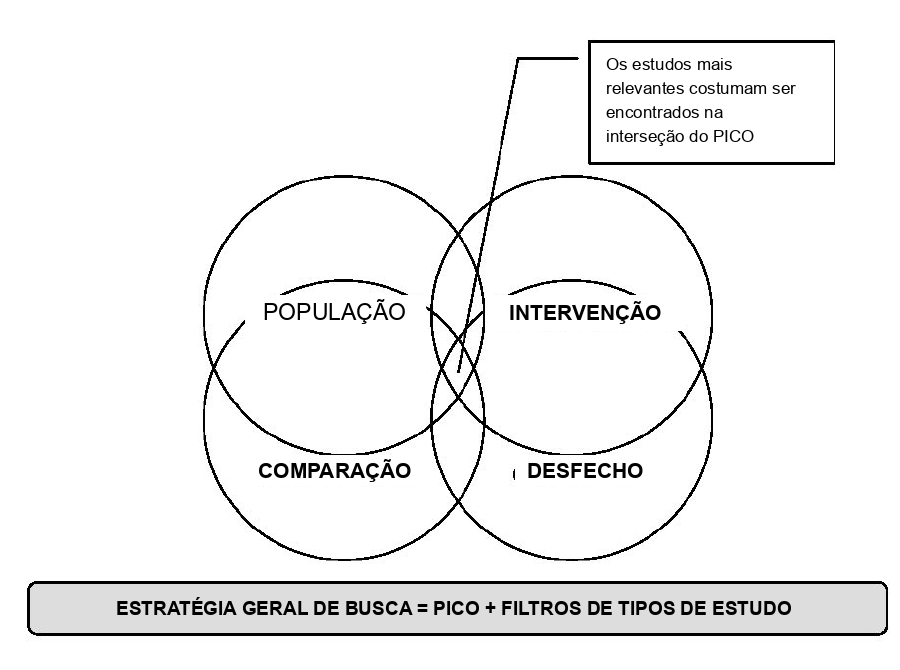
\includegraphics[width=0.68\textwidth]{figuras/pico-pai-2004.png}
	\fonte{Adaptado de \citeonline{pai2004}.}
\end{figure}

\subsection{Definição dos componentes PICOC e string de busca}
\label{subsec:picoc-string-busca}

A formulação da estratégia de busca orientou-se pela adaptação dos elementos do modelo PICOC (\textit{Population, Intervention, Comparison, Outcome, Context}) \cite{pai2004,kitchenham2007}, permitindo delimitar termos centrais e sinônimos relevantes para recuperar estudos que investigam a aplicação de visão computacional e inteligência artificial no diagnóstico da hanseníase. A Tabela~\ref{tab:picoc-termos} detalha os termos centrais e os operadores de expansão semântica definidos para cada faceta do protocolo na ordem do modelo PICOC, formalizando a não aplicabilidade do componente de Comparação.

\begin{table}[htb]
	\centering
	\caption{Componentes do modelo PICOC adaptado e termos de busca}
	\label{tab:picoc-termos}
	\small
	\begin{tabular}{p{2.6cm} p{3.2cm} p{8.2cm}}
		\toprule
		\textbf{Elemento}                            & \textbf{Termo Central}        & \textbf{Sinônimos e Termos Relacionados}                                                                                                                                                                                                                                    \\
		\midrule
		\textbf{População} (\textit{Population})     & \textit{Computer Vision} / IA & \textit{artificial intelligence}, \textit{CNN}, \textit{convolutional neural network*}, \textit{deep learning}, \textit{machine learning}, \textit{neural network*}                                                                                                         \\
		\textbf{Intervenção} (\textit{Intervention}) & Modelos de Aprendizado        & \textit{ResNet*}, \textit{DenseNet*}, \textit{EfficientNet*}, \textit{U-Net}, \textit{UNet}, \textit{Attention U-Net}, \textit{Vision Transformer*}, \textit{ViT}, \textit{ConvNeXt*}, \textit{Swin Transformer*}, \textit{transfer learning}, \textit{supervised learning} \\
		\textbf{Comparação} (\textit{Comparison})    & Não aplicável                 & Não aplicável ao escopo da revisão (mapeamento abrangente sem restrição a grupo de controle ou modelo de referência específico)                                                                                                                                             \\
		\textbf{Resultado} (\textit{Outcome})        & Desempenho e Métricas         & \textit{accuracy}, \textit{AUC}, \textit{ROC-AUC}, \textit{sensitivity}, \textit{specificity}, \textit{precision}, \textit{recall}, \textit{F1-score}, \textit{detection}, \textit{diagnosis}, \textit{evaluation}, \textit{segmentation}                                   \\
		\textbf{Contexto} (\textit{Context})         & Hanseníase                    & \textit{leprosy}, \textit{Hansen disease}, \textit{Hansen's disease}, \textit{hanseniasis}, \textit{skin lesion classification}, \textit{skin lesion segmentation}                                                                                                          \\
		\bottomrule
	\end{tabular}
	\fonte{Autores.}
\end{table}

A partir do mapeamento dos componentes, a string de busca foi estruturada aplicando o operador lógico booleano \texttt{OR} entre os termos e sinônimos no interior de cada dimensão temática, e o operador booleano \texttt{AND} para conectar as quatro facetas fundamentais do protocolo (\textit{População} \texttt{AND} \textit{Intervenção} \texttt{AND} \textit{Resultado} \texttt{AND} \textit{Contexto}). A consulta booleana estruturada é apresentada a seguir:

\begin{center}
	\fbox{
		\begin{minipage}{0.94\textwidth}
			\footnotesize\ttfamily
			( "Computer Vision" OR "artificial intelligence" OR "CNN" OR "convolutional neural network*" OR "deep learning" OR "machine learning" OR "neural network*" ) \\
			\textbf{AND} \\
			( "ResNet*" OR "DenseNet*" OR "EfficientNet*" OR "U-Net" OR "UNet" OR "Vision Transformer*" OR "ViT" OR "transfer learning" OR "supervised learning" OR "Few-shot" ) \\
			\textbf{AND} \\
			( "accuracy" OR "AUC" OR "sensitivity" OR "specificity" OR "precision" OR "recall" OR "F1-score" OR "ROC-AUC" OR "evaluation" OR "detection" OR "segmentation" ) \\
			\textbf{AND} \\
			( "leprosy" OR "Hansen disease" OR "Hansen's disease" OR "hanseniasis" OR "skin lesion classification" OR "skin lesion segmentation" )
		\end{minipage}
	}
\end{center}

\subsection{Prompt estruturado submetido à plataforma Consensus}
\label{subsec:prompt-consensus}

Diferentemente dos motores de busca acadêmicos convencionais baseados exclusivamente na correspondência estrita de operadores booleanos, a plataforma Consensus emprega inteligência artificial para recuperação semântica em grafos de citações e literatura biomédica. Por essa razão, a formulação submetida à ferramenta integrou a questão norteadora principal, as oito perguntas secundárias da revisão e a totalidade dos termos e sinônimos delimitados na matriz PICOC em um \textit{prompt} estruturado em língua inglesa.

O Quadro~\ref{qua:prompt-consensus} reproduz integralmente a solicitação submetida à plataforma Consensus, preservando a sintaxe original, a estrutura das facetas conceituais e os operadores de truncamento aplicados aos termos técnicos.

\lstinputlisting[
	caption={Prompt estruturado em linguagem natural submetido à plataforma Consensus},
	label={qua:prompt-consensus},
	basicstyle=\scriptsize\ttfamily,
	breaklines=true,
	breakatwhitespace=true,
	columns=flexible,
	keepspaces=true,
	frame=single,
	rulecolor=\color{black!30},
	backgroundcolor=\color{black!2},
	xleftmargin=0.5em,
	xrightmargin=0.5em
]{editaveis/prompt-consensus.txt}
\vspace{-0.2cm}\noindent\footnotesize\textbf{Fonte:} Autores.\vspace{0.4cm}

\subsection{Consultas apresentadas pelo Consensus}

Na busca de 25 de setembro de 2026, o Consensus apresentou uma sequência
de consultas em quatro rodadas. A Tabela~\ref{tab:consultas-consensus}
reproduz os textos e indicadores exibidos. Esses indicadores são saídas
internas da ferramenta e não correspondem, por si só, a contagens auditadas
de estudos únicos triados pela dupla.

\begin{longtable}{p{0.08\textwidth}p{0.68\textwidth}r}
	\caption{Consultas e indicadores apresentados pelo Consensus}\label{tab:consultas-consensus}                                                               \\
	\toprule
	Rodada          & Consulta                                                                                                                     & Indicador \\
	\midrule
	\endfirsthead
	\toprule Rodada & Consulta                                                                                                                     & Indicador \\
	\midrule
	\endhead
	1               & deep learning convolutional neural network leprosy Hansen disease skin lesion classification detection diagnosis             & 95,3 mil  \\
	1               & U-Net ResNet EfficientNet Vision Transformer skin lesion segmentation leprosy hanseniasis dermatological pattern recognition & 2,3 mil   \\
	1               & machine learning model performance evaluation accuracy AUC F1 sensitivity specificity leprosy skin image diagnosis           & 63,5 mil  \\
	1               & skin tone fairness demographic subgroup performance dermatology AI model external validation generalization cross-dataset    & 67,4 mil  \\
	2               & leprosy skin image dataset Brazil public health AI diagnosis computer vision                                                 & 26,2 mil  \\
	2               & transfer learning self-supervised semi-supervised learning skin neglected tropical disease leprosy image classification      & 36,6 mil  \\
	2               & WHO skin neglected tropical diseases mobile application telemedicine leprosy detection low-resource settings                 & 63,4 mil  \\
	3               & explainability XAI Grad-CAM interpretable AI leprosy neglected tropical disease skin lesion diagnosis                        & 1,6 mil   \\
	3               & histopathological image analysis acid-fast bacilli detection deep learning leprosy nerve biopsy microscopy                   & 17,6 mil  \\
	4               & leprosy skin image dataset multimodal clinical metadata paucibacillary multibacillary classification AI model                & 3 mil     \\
	4               & reporting standards quality assessment QUADAS CONSORT-AI CLEAR dermatology AI model evaluation systematic review             & 47,8 mil  \\
	\bottomrule
\end{longtable}

A pesquisa na \textit{Consensus} foi feita
no modo \textit{Deep}, com 19 etapas. A plataforma descreve \textit{Retrieved}
de 425,4 mil como o total de trabalhos encontrados nas buscas;
\textit{Eligible} de mil como os trabalhos considerados relevantes após a
deduplicação da ferramenta; e \textit{Included} de 100 como os trabalhos
selecionados pela ferramenta para a análise final. Essas descrições não
esclarecem integralmente os critérios e procedimentos internos utilizados.

Após a segunda rodada, o histórico indica uma expansão por grafo de citações
a partir de dez trabalhos iniciais, com 662 trabalhos associados; após a
terceira, indica a leitura de 12 resumos; antes da síntese, registra a leitura
de resumos e PDFs de 100 trabalhos. A busca também
foi ampliada para temas relacionados, como dermatologia geral, equidade,
saúde móvel, microscopia, histopatologia e diretrizes de relato. A presença
de uma referência na saída da ferramenta não significa que ela atenda aos
critérios da revisão. Os 100 registros retornados pelo Consensus foram salvos
pelos autores e compuseram, juntamente com os registros obtidos na busca
complementar pelo Claude, a base inicial submetida à deduplicação e à triagem.

\section{Realização da busca e seleção dos artigos}
\label{sec:execucao-busca-selecao}

Para conferir rigor metodológico, reprodutibilidade e transparência à revisão estruturada da literatura, o processo de identificação, deduplicação, triagem por título e resumo, avaliação de elegibilidade e extração foi conduzido por meio de um fluxo de trabalho assistido por ferramentas de inteligência artificial especializadas, articuladas sob contínuo julgamento crítico e validação por pares da dupla de pesquisadores.

A Figura~\ref{fig:fluxo-metodologico-ia} ilustra o fluxo metodológico integrado, evidenciando as seis etapas da revisão, os volumes documentais em cada transição e a atuação específica de cada ferramenta de apoio (\textit{Consensus}, \textit{Claude}, \textit{JevReviewer} e \textit{Evidentia Review}).

\begin{figure}[htbp]
	\centering
	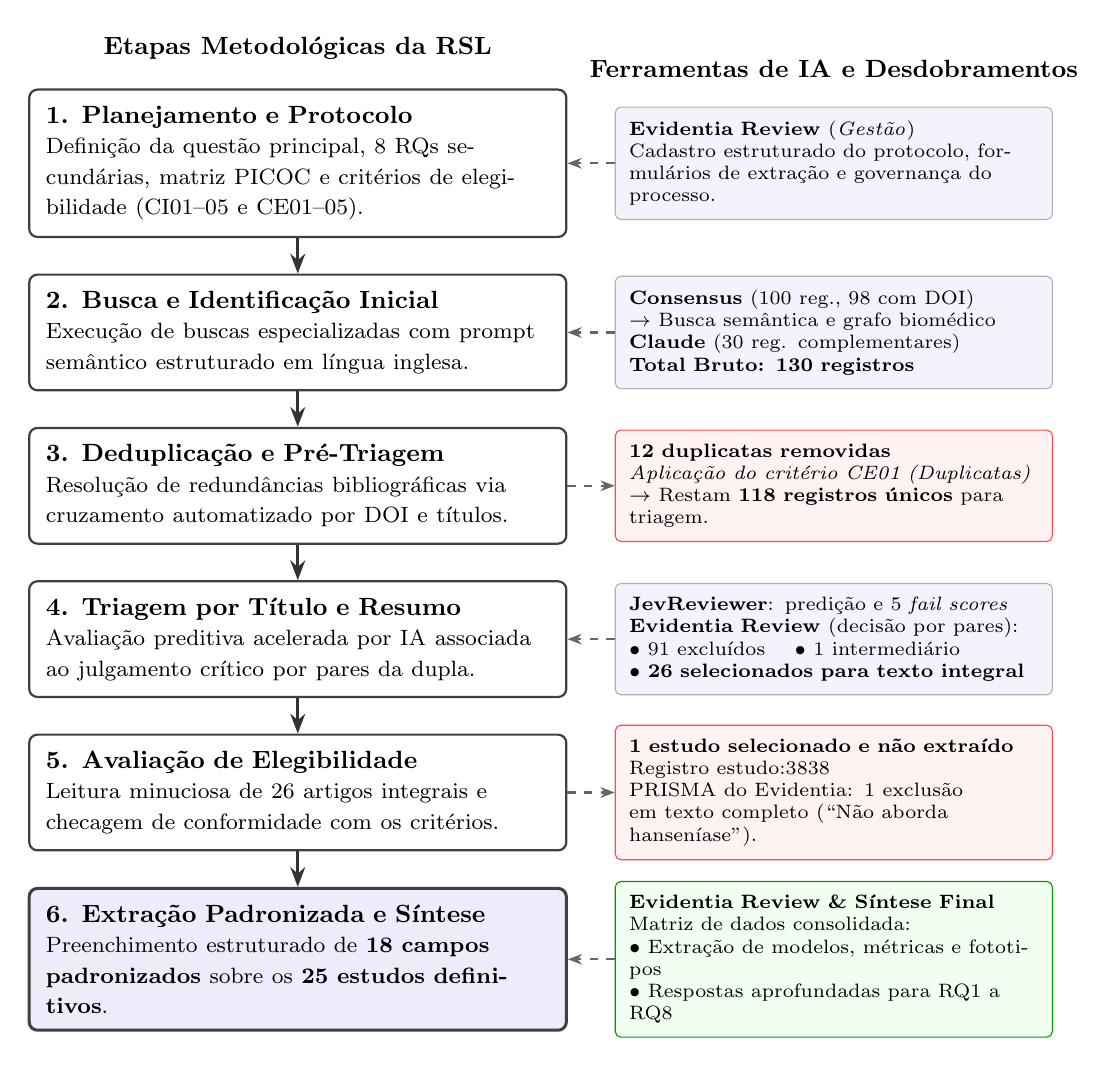
\begin{tikzpicture}[
		stage/.style={
				draw=black!75,
				fill=white,
				thick,
				rounded corners=3pt,
				text width=6.4cm,
				font=\small,
				inner sep=6pt
			},
		tool/.style={
				draw=black!30,
				fill=blue!5,
				rounded corners=2pt,
				text width=5.2cm,
				font=\scriptsize,
				inner sep=5pt
			},
		excl/.style={
				draw=red!70,
				fill=red!5,
				rounded corners=2pt,
				text width=5.2cm,
				font=\scriptsize,
				inner sep=5pt
			},
		finalstage/.style={
				draw=black!75,
				fill=blue!8,
				line width=1.1pt,
				rounded corners=3pt,
				text width=6.4cm,
				font=\small,
				inner sep=6pt
			},
		mainarrow/.style={
		-{Stealth[length=2.5mm]},
		line width=1.2pt,
		draw=black!80
		},
		conn/.style={
		-{Stealth[length=1.8mm]},
		draw=black!60,
		dashed,
		thick
		}
		]

		% 1. Protocolo
		\node[stage] (s1) {\textbf{1. Planejamento e Protocolo}\\
			\footnotesize Definição da questão principal, 8 RQs secundárias, matriz PICOC e critérios de elegibilidade (CI01--05 e CE01--05).};

		\node[tool, right=0.6cm of s1] (t1) {\textbf{Evidentia Review} (\textit{Gestão})\\
			Cadastro estruturado do protocolo, formulários de extração e governança do processo.};

		% Headers
		\node[font=\bfseries\small, above=0.25cm of s1] (h1) {Etapas Metodológicas da RSL};
		\node[font=\bfseries\small, above=0.25cm of t1] (h2) {Ferramentas de IA e Desdobramentos};

		% 2. Busca e Identificação
		\node[stage, below=0.45cm of s1] (s2) {\textbf{2. Busca e Identificação Inicial}\\
			\footnotesize Execução de buscas especializadas com prompt semântico estruturado em língua inglesa.};

		\node[tool] (t2) at (s2 -| t1) {\textbf{Consensus} (100 reg., 98 com DOI)\\
			$\rightarrow$ Busca semântica e grafo biomédico\\
			\textbf{Claude} (30 reg. complementares)\\
			\textbf{Total Bruto: 130 registros}};

		% 3. Deduplicação
		\node[stage, below=0.45cm of s2] (s3) {\textbf{3. Deduplicação e Pré-Triagem}\\
			\footnotesize Resolução de redundâncias bibliográficas via cruzamento automatizado por DOI e títulos.};

		\node[excl] (t3) at (s3 -| t1) {\textbf{12 duplicatas removidas}\\
			\textit{Aplicação do critério CE01 (Duplicatas)}\\
			$\rightarrow$ Restam \textbf{118 registros únicos} para triagem.};

		% 4. Triagem Título/Resumo
		\node[stage, below=0.45cm of s3] (s4) {\textbf{4. Triagem por Título e Resumo}\\
			\footnotesize Avaliação preditiva acelerada por IA associada ao julgamento crítico por pares da dupla.};

		\node[tool] (t4) at (s4 -| t1) {\textbf{JevReviewer}: predição e 5 \textit{fail scores}\\
			\textbf{Evidentia Review} (decisão por pares):\\
			$\bullet$ 91 excluídos \quad $\bullet$ 1 intermediário\\
			$\bullet$ \textbf{26 selecionados para texto integral}};

		% 5. Leitura na Íntegra
		\node[stage, below=0.45cm of s4] (s5) {\textbf{5. Avaliação de Elegibilidade}\\
			\footnotesize Leitura minuciosa de 26 artigos integrais e checagem de conformidade com os critérios.};

		\node[excl] (t5) at (s5 -| t1) {\textbf{1 estudo selecionado e não extraído}\\
			Registro~\estudo{38}\\
			PRISMA do Evidentia: 1 exclusão em texto completo (``Não aborda hanseníase'').};

		% 6. Extração e Síntese
		\node[finalstage, below=0.45cm of s5] (s6) {\textbf{6. Extração Padronizada e Síntese}\\
			\footnotesize Preenchimento estruturado de \textbf{18 campos padronizados} sobre os \textbf{25 estudos definitivos}.};

		\node[tool, draw=green!60!black, fill=green!6] (t6) at (s6 -| t1) {\textbf{Evidentia Review \& Síntese Final}\\
			Matriz de dados consolidada:\\
			$\bullet$ Extração de modelos, métricas e fototipos\\
			$\bullet$ Respostas aprofundadas para RQ1 a RQ8};

		% Downward main arrows
		\draw[mainarrow] (s1) -- (s2);
		\draw[mainarrow] (s2) -- (s3);
		\draw[mainarrow] (s3) -- (s4);
		\draw[mainarrow] (s4) -- (s5);
		\draw[mainarrow] (s5) -- (s6);

		% Horizontal connections
		\draw[conn] (t1) -- (s1);
		\draw[conn] (t2) -- (s2);
		\draw[conn] (s3) -- (t3);
		\draw[conn] (t4) -- (s4);
		\draw[conn] (s5) -- (t5);
		\draw[conn] (t6) -- (s6);

	\end{tikzpicture}
	\caption{Fluxo metodológico da Revisão Estruturada da Literatura assistido por ferramentas de inteligência artificial}
	\label{fig:fluxo-metodologico-ia}
	\fonte{Autores.}
\end{figure}

\subsection{Busca e identificação dos registros}

O protocolo da revisão foi organizado no Evidentia a partir da questão de
pesquisa e dos componentes do PICOC. Esses elementos foram utilizados em
uma solicitação em inglês ao Consensus, sem a inclusão dos critérios de
seleção no texto do \textit{prompt}. Em 25 de setembro de 2026, a
ferramenta retornou uma lista de 100 referências, que foi salva pelos autores,
das quais 98 tinham DOI informado. Foi registrada também uma busca complementar por meio do Claude, da qual
foram reunidas 30 referências. A data, o \textit{prompt}, o modelo, a configuração e a lista completa
dessa busca complementar ainda precisam ser confirmados. Embora o protocolo
também registre a Scopus como fonte, não há comprovação de uma busca separada
nessa base na etapa descrita.

As duas listas somaram 130 registros e,
após a remoção de duplicatas, permaneceram 118 para triagem. A diferença
entre esses totais corresponde a 12 registros removidos; entretanto, os
pares considerados duplicados e o procedimento usado para identificá-los
ainda não foram integralmente documentados. O conjunto bibliográfico disponível contém 129 entradas. Na comparação
com os 118 registros triados, onze entradas não aparecem no conjunto de triagem e apresentam o mesmo DOI de outras entradas nele
representadas. Essa comparação permite identificar 11 pares de
registros com DOI coincidente, mas não identifica um eventual décimo
segundo registro removido nem comprova, isoladamente, quando cada par
foi deduplicado. A diferença entre as 129 entradas identificadas e os
130 registros informados no relato permanece a esclarecer. Os
indicadores internos apresentados pelo Consensus não foram tratados
como quantidades auditadas de estudos únicos examinados pelos pesquisadores.
Após a reunião dos registros do Consensus e do Claude e a deduplicação,
o Jev apoiou a classificação preliminar e os autores registraram as decisões
de triagem no Evidentia, como descrito na subseção seguinte.

\subsection{Critérios de seleção}

Os critérios de inclusão foram: disponibilidade do texto completo (CI01);
uso de visão computacional, aprendizado de máquina ou aprendizado profundo
para detectar, classificar, identificar ou segmentar manifestações
cutâneas humanas associadas à hanseníase (CI02); relato ou síntese de
evidências de avaliação de métodos de inteligência artificial para
hanseníase, incluindo experimentos, testes, validação ou comparação de
desempenho (CI03); uso, análise ou revisão de fotografias clínicas ou
imagens dermatoscópicas de lesões cutâneas humanas associadas à hanseníase
(CI04); e inclusão da hanseníase entre as condições avaliadas em trabalhos
que abordam múltiplas doenças (CI05). A formulação preservada do CI03 foi
recebida truncada após ``resultados de estu''; o trecho descrito acima
resume apenas a parte legível e sua redação integral deve ser confirmada.
Os critérios abrangem estudos primários e revisões, que devem ser
distinguidos durante a extração.

Foram informados os seguintes critérios de exclusão: registro duplicado de
artigo já considerado (CE01); publicação anterior a 2020 (CE02); texto
completo em idioma diferente de inglês ou português (CE03); uso exclusivo
de inteligência artificial generativa como intervenção (CE04); e ausência
de abordagem da hanseníase (CE05). A verificação de disponibilidade e
idioma do texto completo pode depender de consulta além do título e do
resumo, enquanto data e duplicidade também dependem dos metadados.

\subsection{Triagem e seleção para leitura integral}

O Jev Reviewer foi utilizado como apoio à classificação preliminar dos
118 registros. Para cada registro, suas sugestões são acompanhadas de
valores associados ao não atendimento de cinco critérios:
\begin{enumerate}
	\item Abordar a hanseníase como condição investigada ou avaliada,
	      isoladamente ou entre outras doenças; uma menção apenas introdutória não
	      atende a esse critério.
	\item Utilizar fotografias clínicas ou imagens dermatoscópicas de
	      manifestações cutâneas humanas associadas à hanseníase, ou revisar estudos
	      que utilizam essas imagens.
	\item Aplicar ou analisar métodos de visão computacional, aprendizado de
	      máquina ou aprendizado profundo para detectar, classificar, identificar
	      ou segmentar essas manifestações nas imagens, incluindo revisões dessas
	      aplicações.
	\item Relatar ou sintetizar evidências de avaliação desses métodos, como
	      experimentos, testes, validação, comparação de desempenho ou resultados
	      de estudos.
	\item Não se limitar exclusivamente à inteligência artificial generativa
	      como intervenção.
\end{enumerate}

Esses cinco critérios descrevem o que foi avaliado pelo Jev; eles não
substituem os critérios gerais de inclusão e exclusão da revisão. Os valores
de \texttt{fails} acompanham a avaliação automatizada e não registram, por
si sós, a justificativa da decisão dos pesquisadores. Após a classificação
preliminar, a dupla relatou ter revisado os registros por título e resumo,
com as decisões registradas no Evidentia. A documentação não esclarece se
ambos avaliaram todos os registros de maneira independente. A avaliação por
dois ou mais pesquisadores, ao menos para uma amostra, é recomendada por
\citeonline{wohlin2024}; essa recomendação não demonstra que ela
foi executada neste trabalho.

As sugestões do Jev para os 118 registros foram: duas de inclusão, 15 incertas e 101 de exclusão.
O cruzamento por título entre as sugestões e as decisões do Evidentia
identificou correspondência para todos os registros. Entre os 26 com
situação de inclusão no Evidentia, dois tinham sugestão de inclusão do
Jev, 11 tinham sugestão incerta e 13 tinham sugestão de exclusão. Entre
os 91 excluídos no Evidentia, 87 tinham sugestão de exclusão e quatro
tinham sugestão incerta. O registro restante, classificado como
intermediário no Evidentia, tinha sugestão de exclusão pelo Jev. Assim,
as sugestões automáticas são distintas das decisões de triagem. A data de
execução, o modelo, a configuração completa e a versão da ferramenta não
foram identificados; os cinco critérios exibidos acima, por sua vez, estão
registrados nas avaliações disponíveis.

Os estados intermediários da triagem registram, em uma etapa, 12 inclusões,
32 exclusões, 15 decisões intermediárias e 59 registros sem decisão. Em
outro estado foram observadas 19 inclusões, 40 exclusões e os mesmos 59
registros sem decisão; as 15 decisões intermediárias passaram a sete
inclusões e oito exclusões. As datas das decisões preenchidas indicam
28 de setembro de 2026, mas não registram horário de cada decisão. Esses
estados intermediários não devem ser confundidos com o resultado
consolidado descrito a seguir.

No Evidentia, 91 registros apresentam decisão de exclusão,
26 de inclusão e uma decisão intermediária, totalizando 118 registros (Tabela~\ref{tab:registros-118}, Apêndice~\ref{apend:registros}).
Esse último registro, \textit{Leprosy Screening Based on Artificial
	Intelligence: Development of a Cross-Platform App} (registro~\estudo{9}), apresenta duas
decisões individuais de exclusão, mas sua decisão consolidada foi
registrada manualmente como intermediária. Em outro registro,
\textit{Leprosy lesion recognition using convolutional neural networks} (registro~\estudo{90}),
houve uma decisão individual de inclusão e uma de exclusão; o conflito
foi resolvido manualmente com decisão consolidada de exclusão. Os demais
116 registros possuem decisão consolidada automática, segundo o campo
correspondente no Evidentia. Essa classificação descreve o mecanismo de
consolidação registrado pelo sistema e não identifica uma revisão
independente por ambos os pesquisadores para cada artigo.

A decomposição 91 exclusões, 26 inclusões e uma decisão intermediária
esclarece a diferença observada no registro anterior: 118 menos 26 é 92,
mas esse resultado reúne os 91 excluídos e o registro intermediário.
Assim, não se deve representar a diferença de 92 como 92 exclusões.
Os 26 registros com situação de inclusão na triagem constituíram o conjunto
encaminhado à leitura integral. Após a análise aprofundada dos textos completos e
verificação dos critérios de elegibilidade no formulário de extração, 25 estudos foram
confirmados e integralmente extraídos. O registro~\estudo{38} está entre os 26 e não consta
da extração final. As fontes registram coisas diferentes a seu respeito: o relatório PRISMA do Evidentia
(03/11/2026) registra uma exclusão em texto completo, com o motivo ``Não aborda hanseníase''; o título do
artigo trata de imagens dermatológicas geradas por inteligência artificial; e as planilhas de triagem não
registram motivo de exclusão para esse registro (decisão de inclusão).

A Figura~\ref{fig:fluxo-triagem} sintetiza as quantidades descritas nesta
seção; os 118 registros e sua situação estão listados na Tabela~\ref{tab:registros-118} (Apêndice~\ref{apend:registros}). A indicação de 12 registros removidos corresponde à diferença entre
130 e 118, decorrente da deduplicação das fontes de identificação. O processo
culminou na seleção definitiva de 25 estudos para extração e síntese.
Segundo o relatório PRISMA do Evidentia, dos 91 registros excluídos por título e resumo, 67 têm o motivo
``Não aborda hanseníase'' e 24 não têm motivo registrado; as planilhas de triagem não registram o motivo
de cada exclusão.

\begin{figure}[htbp]
	\centering
	\caption{Fluxo de identificação, triagem e inclusão dos estudos}
	\label{fig:fluxo-triagem}
	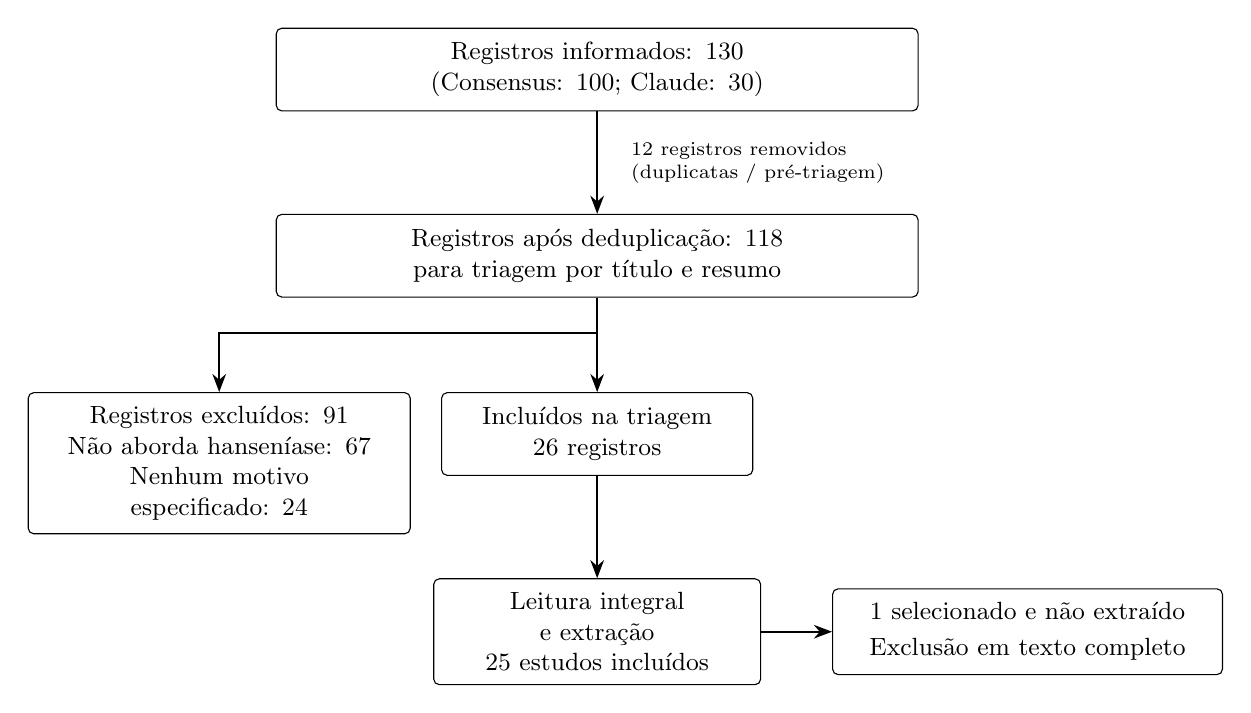
\begin{tikzpicture}[
		box/.style={draw,rounded corners=2pt,align=center,minimum height=1.05cm,inner sep=5pt,font=\small},
		wide/.style={box,text width=7.8cm},
		arrow/.style={-{Stealth[length=2.3mm]},thick}
		]
		\node[wide] (identified) {Registros informados: 130\\(Consensus: 100; Claude: 30)};
		\node[wide,below=1.3cm of identified] (screened) {Registros após deduplicação: 118\\para triagem por título e resumo};
		\draw[arrow] (identified) -- node[right=3mm,align=left,font=\scriptsize,text width=4.2cm] {12 registros removidos\\(duplicatas / pré-triagem)} (screened);

		\node[box,text width=4.5cm,below=1.2cm of screened,xshift=-4.8cm] (excluded) {Registros excluídos: 91\\Não aborda hanseníase: 67\\Nenhum motivo especificado: 24};
		\node[box,text width=3.6cm,below=1.2cm of screened] (included) {Incluídos na triagem\\26 registros};
		\draw[arrow] (screened.south) -- ++(0,-0.45) -| (excluded.north);
		\draw[arrow] (screened.south) -- (included.north);

		\node[box,text width=3.8cm,below=1.3cm of included] (fulltext) {Leitura integral\\e extração\\25 estudos incluídos};
		\node[box,text width=4.6cm,right=0.9cm of fulltext] (not_extracted) {1 selecionado e não extraído\\[2pt]Exclusão em texto completo};
		\draw[arrow] (included.south) -- (fulltext.north);
		\draw[arrow] (fulltext.east) -- (not_extracted.west);
	\end{tikzpicture}
	\fonte{Autores.}
\end{figure}

\begin{table}[htb]
	\centering
	\caption{Quantidades documentadas na identificação, triagem e inclusão dos estudos}
	\label{tab:fluxo-selecao-estudos}
	\begin{tabular}{p{0.66\textwidth} r}
		\toprule
		Etapa ou registro                                       & Quantidade \\
		\midrule
		Referências informadas do Consensus                     & 100        \\
		Referências informadas do Claude                        & 30         \\
		Registros reunidos                                      & 130        \\
		Registros removidos na pré-triagem (duplicatas)         & 12         \\
		Registros submetidos à triagem no Evidentia             & 118        \\
		Excluídos na triagem por título e resumo                & 91         \\
		Incluídos na triagem para leitura integral              & 26         \\
		Decisão intermediária (avaliada e resolvida)            & 1          \\
		Selecionado para leitura integral e não extraído        & 1          \\
		Estudos incluídos definitivamente com extração completa & 25         \\
		\bottomrule
	\end{tabular}
	\fonte{Autores.}
\end{table}

O formulário de extração no sistema Evidentia reúne os 25 estudos incluídos
definitivamente após a leitura integral e verificação de elegibilidade, com todos os seus
18 campos padronizados integralmente preenchidos. Entre os 26 registros pré-selecionados na
triagem, o estudo \textit{AI-generated dermatologic images show deficient skin tone
	diversity and poor diagnostic accuracy: An experimental study} (registro~\estudo{38}) não
integrou a extração final; o relatório PRISMA do Evidentia registra uma exclusão em texto completo, com o
motivo ``Não aborda hanseníase'', e as planilhas de triagem não registram motivo de exclusão por registro.

Quanto à rastreabilidade do processo de seleção, os motivos de exclusão constam apenas de forma agregada no
relatório PRISMA do Evidentia: dos 91 registros excluídos por título e resumo, 67 com o motivo
``Não aborda hanseníase'' e 24 sem motivo registrado; as planilhas de triagem não registram o motivo de
cada exclusão. Com a resolução das divergências e a conclusão
da leitura aprofundada, consolidou-se o conjunto definitivo de 25 estudos que subsidiam
as análises empíricas desta monografia.

\subsection{Extração e síntese das evidências}

Conforme \citeonline{wohlin2024}, o formulário de extração
deve ser orientado pelas questões de pesquisa e permitir o registro das
características dos estudos e dos dados necessários à síntese. Neste
trabalho, o formulário foi organizado para registrar título, autores,
ano, fonte, tipo de estudo e veículo, além das respostas detalhadas às questões da
revisão: técnicas de visão computacional, bases de dados, características das populações, manifestações cutâneas, quantidade de
imagens, métodos e procedimentos de avaliação, métricas, resultados obtidos, informações sobre tons de pele,
modelos de inteligência artificial, avaliação de generalização, métodos de validação e limitações relatadas. A extração completa dos 25 estudos permitiu correlacionar sistematicamente cada achado com as páginas e tabelas de origem, distinguindo rigorosamente estudos primários e revisões para evitar atribuições indevidas de métricas secundárias.

A síntese apresentada a seguir distingue formalmente as tarefas de classificação diagnóstica, detecção e segmentação de feridas, bem
como compara os desempenhos globais multiclasse com os resultados específicos obtidos para hanseníase. As lacunas documentadas a respeito da ausência de estratificação por tons de pele e as limitações de validação externa em bases independentes evidenciam a relevância científica do tema e balizam a discussão sobre a viabilidade e os riscos de implantação dessas ferramentas no SUS.

\section{Resultados da revisão}
\label{sec:resultados-revisao}

Esta seção apresenta a síntese qualitativa e quantitativa das evidências
extraídas dos 25 estudos primários e secundários incluídos definitivamente
na revisão estruturada da literatura. Os dados foram extraídos a partir de
formulário estruturado no Evidentia Review, composto por 18 campos padronizados,
permitindo responder detalhadamente a cada uma das questões secundárias de
pesquisa estabelecidas no protocolo.

\nocite{fernandes2024,andrade2025,deps2024,deps2026,yotsu2023,jitendra2024deep,nyatte2022,vargasclavijo2025,goswami2026,prayitno2026,sall2025,ahikpa2025,barbieri2022,baweja2023,pons2026,innocent2026,beesetty2023,jitendra2024heuristic,gawali2024,yotsu2025,sanchez2024,mehta2026,eita2025,jaikishore2021,banerjee2023,baweja2016,souza2021,joerg2025}

Os estudos incluídos são referidos nesta monografia por identificador (ID), de E01 a E25, que remete, por hiperligação, à linha correspondente da Tabela~\ref{tab:estudos-incluidos}, onde constam autores, ano, título, veículo, tipo de veículo, grupo e DOI. Os registros da triagem que não integram os 25 estudos incluídos são referidos por identificador numérico de 1 a 118 (por exemplo, registro~\estudo{9}), que remete à Tabela~\ref{tab:registros-118} (Apêndice~\ref{apend:registros}), com a totalidade dos 118 registros encontrados na busca e suas respectivas situações.

\begingroup
\scriptsize
\setlength{\tabcolsep}{2.5pt}
\renewcommand{\arraystretch}{1.1}
\begin{longtable}{@{}lp{2.7cm}lp{3.6cm}p{2.7cm}llp{2.1cm}@{}}
	\caption[Estudos inclu\'idos na revis\~ao, com identificador (ID)]{Estudos inclu\'idos na revis\~ao (n = 25), com identificador (ID). Grupos: A, desenvolve e avalia modelo; B, valida\c{c}\~ao externa de modelo de terceiros; C, protocolo; D, revis\~ao, perspectiva ou editorial}\label{tab:estudos-incluidos}                                                                                                                                                                                                                                                                                                \\
	\toprule
	\textbf{ID}                   & \textbf{Autores}                             & \textbf{Ano} & \textbf{T\'itulo}                                                                                                                                                                                                   & \textbf{Ve\'iculo}                                                                                 & \textbf{Tipo} & \textbf{Gr.} & \textbf{DOI}                                                                                                                                              \\
	\midrule
	\endfirsthead
	\multicolumn{8}{l}{\scriptsize\textit{Tabela~\ref{tab:estudos-incluidos} (continua\c{c}\~ao)}}                                                                                                                                                                                                                                                                                                                                                                                                                                                                                                                    \\
	\toprule
	\textbf{ID}                   & \textbf{Autores}                             & \textbf{Ano} & \textbf{T\'itulo}                                                                                                                                                                                                   & \textbf{Ve\'iculo}                                                                                 & \textbf{Tipo} & \textbf{Gr.} & \textbf{DOI}                                                                                                                                              \\
	\midrule
	\endhead
	\midrule
	\multicolumn{8}{r}{\scriptsize\textit{continua na pr\'oxima p\'agina}}                                                                                                                                                                                                                                                                                                                                                                                                                                                                                                                                            \\
	\endfoot
	\bottomrule
	\endlastfoot
	\hypertarget{estudo:E01}{}E01 & FERNANDES, J. R. N. et al.                   & 2024         & Artificial Intelligence on Diagnostic Aid of Leprosy: A Systematic Literature Review                                                                                                                                & Journal of Clinical Medicine                                                                       & Revista       & D            & \href{https://doi.org/10.3390/jcm13010180}{10.\allowbreak{}3390/\allowbreak{}jcm13010180}                                                                 \\
	\hypertarget{estudo:E02}{}E02 & ANDRADE, H. G. V. de et al.                  & 2025         & On the usage of artificial intelligence in leprosy care: A systematic literature review                                                                                                                             & PLOS Computational Biology                                                                         & Revista       & D            & \href{https://doi.org/10.1371/journal.pcbi.1012550}{10.\allowbreak{}1371/\allowbreak{}journal.\allowbreak{}pcbi.\allowbreak{}1012550}                     \\
	\hypertarget{estudo:E03}{}E03 & DEPS, P. D. et al.                           & 2024         & The potential role of artificial intelligence in the clinical management of Hansen's disease (leprosy)                                                                                                              & Frontiers in Medicine                                                                              & Revista       & D            & \href{https://doi.org/10.3389/fmed.2024.1338598}{10.\allowbreak{}3389/\allowbreak{}fmed.\allowbreak{}2024.\allowbreak{}1338598}                           \\
	\hypertarget{estudo:E04}{}E04 & DEPS, P. et al.                              & 2026         & Independent assessment of the WHO Skin Neglected Tropical Diseases application for leprosy detection                                                                                                                & Revista Panamericana de Salud Pública                                                              & Revista       & B            & \href{https://doi.org/10.26633/RPSP.2026.40}{10.\allowbreak{}26633/\allowbreak{}RPSP.\allowbreak{}2026.\allowbreak{}40}                                   \\
	\hypertarget{estudo:E05}{}E05 & YOTSU, R. R. et al.                          & 2023         & Deep learning for AI-based diagnosis of skin-related neglected tropical diseases: A pilot study                                                                                                                     & PLOS Neglected Tropical Diseases                                                                   & Revista       & A            & \href{https://doi.org/10.1371/journal.pntd.0011230}{10.\allowbreak{}1371/\allowbreak{}journal.\allowbreak{}pntd.\allowbreak{}0011230}                     \\
	\hypertarget{estudo:E06}{}E06 & JITENDRA, R. et al.                          & 2024         & Deep Semantic Segmentation Assisted Region-of-Interest Sensitive Deep Spatio-Textural Feature Learning Framework for Leprosy Detection and Classification                                                           & SN Computer Science                                                                                & Revista       & A            & \href{https://doi.org/10.1007/s42979-024-03054-2}{10.\allowbreak{}1007/\allowbreak{}s42979-024-03054-2}                                                   \\
	\hypertarget{estudo:E07}{}E07 & STEYVE, N. et al.                            & 2022         & Optimized real-time diagnosis of neglected tropical diseases by automatic recognition of skin lesions                                                                                                               & Informatics in Medicine Unlocked                                                                   & Revista       & A            & \href{https://doi.org/10.1016/j.imu.2022.101078}{10.\allowbreak{}1016/\allowbreak{}j.\allowbreak{}imu.\allowbreak{}2022.\allowbreak{}101078}              \\
	\hypertarget{estudo:E08}{}E08 & VARGAS-CLAVIJO, M. et al.                    & 2025         & Evaluating Advanced Machine Learning Models for Histopathological Diagnosis of Hansen Disease                                                                                                                       & The American Journal of Dermatopathology                                                           & Revista       & A            & \href{https://doi.org/10.1097/dad.0000000000002875}{10.\allowbreak{}1097/\allowbreak{}dad.\allowbreak{}0000000000002875}                                  \\
	\hypertarget{estudo:E09}{}E09 & GOSWAMI, A.; VERMA, S.; MARAK, A.            & 2026         & Unveiling leprosy through machines: a review of artificial intelligence in a neglected tropical disease                                                                                                             & Portuguese Journal of Dermatology and Venereology                                                  & Revista       & D            & \href{https://doi.org/10.24875/PJDV.25000080}{10.\allowbreak{}24875/\allowbreak{}PJDV.\allowbreak{}25000080}                                              \\
	\hypertarget{estudo:E10}{}E10 & PRAYITNO, B.; TRIYANTO, E.                   & 2026         & Utilization of digital health in the screening, diagnosis, and management of Morbus Hansen                                                                                                                          & Malahayati International Journal of Nursing and Health Science                                     & Revista       & D            & \href{https://doi.org/10.33024/minh.v9i4.3415}{10.\allowbreak{}33024/\allowbreak{}minh.\allowbreak{}v9i4.\allowbreak{}3415}                               \\
	\hypertarget{estudo:E11}{}E11 & SALL, D. et al.                              & 2025         & Potential of the World Health Organization's Skin NTDs App to Support and Improve the Detection of Skin-Related Neglected Tropical Diseases: Protocol for a Performance Evaluation and Feasibility Study in Senegal & JMIR Research Protocols                                                                            & Revista       & C            & \href{https://doi.org/10.2196/69420}{10.\allowbreak{}2196/\allowbreak{}69420}                                                                             \\
	\hypertarget{estudo:E12}{}E12 & AHIKPA, E. D.; HIMABINDU, K.                 & 2025         & A Machine Learning-Based Diagnosis of Leprosy: Study                                                                                                                                                                & 2025 IEEE International Conference on Emerging Trends in Computing and Communication (ETCOM)       & Conferência   & D            & \href{https://doi.org/10.1109/ETCOM66606.2025.11436464}{10.\allowbreak{}1109/\allowbreak{}ETCOM66606.\allowbreak{}2025.\allowbreak{}11436464}             \\
	\hypertarget{estudo:E13}{}E13 & BARBIERI, R. R. et al.                       & 2022         & Reimagining leprosy elimination with AI analysis of a combination of skin lesion images with demographic and clinical data                                                                                          & The Lancet Regional Health -- Americas                                                             & Revista       & A            & \href{https://doi.org/10.1016/j.lana.2022.100192}{10.\allowbreak{}1016/\allowbreak{}j.\allowbreak{}lana.\allowbreak{}2022.\allowbreak{}100192}            \\
	\hypertarget{estudo:E14}{}E14 & BAWEJA, A. K.; ADITYA, S.; KANCHANA, M.      & 2023         & Leprosy Diagnosis using Explainable Artificial Intelligence Techniques                                                                                                                                              & 2023 International Conference on Sustainable Computing and Data Communication Systems (ICSCDS)     & Conferência   & A            & \href{https://doi.org/10.1109/ICSCDS56580.2023.10104958}{10.\allowbreak{}1109/\allowbreak{}ICSCDS56580.\allowbreak{}2023.\allowbreak{}10104958}           \\
	\hypertarget{estudo:E15}{}E15 & PONS, J. S. et al.                           & 2026         & The World Health Organization skin neglected tropical diseases app: A dynamic capacity-building training tool enhanced with artificial intelligence                                                                 & Journal of Investigative Dermatology                                                               & Revista       & A            & \href{https://doi.org/10.1016/j.jid.2026.03.043}{10.\allowbreak{}1016/\allowbreak{}j.\allowbreak{}jid.\allowbreak{}2026.\allowbreak{}03.\allowbreak{}043} \\
	\hypertarget{estudo:E16}{}E16 & INNOCENT, D. C. et al.                       & 2026         & Explainable AI for differential diagnosis of skin-manifesting neglected tropical diseases (NTDS) in darker skin tones                                                                                               & BMC Artificial Intelligence                                                                        & Revista       & D            & \href{https://doi.org/10.1186/s44398-026-00033-w}{10.\allowbreak{}1186/\allowbreak{}s44398-026-00033-w}                                                   \\
	\hypertarget{estudo:E17}{}E17 & BEESETTY, R. et al.                          & 2023         & Leprosy Skin Lesion Detection: An AI Approach Using Few Shot Learning in a Small Clinical Dataset                                                                                                                   & Indian Journal of Leprosy                                                                          & Revista       & A            & não informado na fonte                                                                                                                                    \\
	\hypertarget{estudo:E18}{}E18 & JITENDRA, R. et al.                          & 2024         & Heuristic Segmentation Assisted Deep-Spatial Feature Learning Model for Leprosy Detection                                                                                                                           & SN Computer Science                                                                                & Revista       & A            & \href{https://doi.org/10.1007/s42979-024-03053-3}{10.\allowbreak{}1007/\allowbreak{}s42979-024-03053-3}                                                   \\
	\hypertarget{estudo:E19}{}E19 & GAWALI, C. J.; SUBBULAKSHMI, S.              & 2024         & Enhancing Diagnosis of Infectious Skin Disease: A Professional Approach using Deep Learning for Leprosy Detection                                                                                                   & 2024 15th International Conference on Computing Communication and Networking Technologies (ICCCNT) & Conferência   & A            & \href{https://doi.org/10.1109/ICCCNT61001.2024.10725616}{10.\allowbreak{}1109/\allowbreak{}ICCCNT61001.\allowbreak{}2024.\allowbreak{}10725616}           \\
	\hypertarget{estudo:E20}{}E20 & YOTSU, R. R. et al.                          & 2025         & Harnessing artificial intelligence for skin-related neglected tropical diseases (skin NTDs): opportunities, challenges and future directions                                                                        & International Health                                                                               & Revista       & D            & \href{https://doi.org/10.1093/inthealth/ihaf068}{10.\allowbreak{}1093/\allowbreak{}inthealth/\allowbreak{}ihaf068}                                        \\
	\hypertarget{estudo:E21}{}E21 & SANCHEZ, K. et al.                           & 2024         & Co2Wounds-V2: Extended Chronic Wounds Dataset from Leprosy Patients                                                                                                                                                 & 2024 IEEE International Conference on Image Processing (ICIP)                                      & Conferência   & A            & \href{https://doi.org/10.1109/ICIP51287.2024.10647641}{10.\allowbreak{}1109/\allowbreak{}ICIP51287.\allowbreak{}2024.\allowbreak{}10647641}               \\
	\hypertarget{estudo:E22}{}E22 & MEHTA, J. et al.                             & 2026         & Integrative Image Processing Framework for Enhanced Detection of Leprosy-Associated Chronic Wounds                                                                                                                  & The International Journal of Lower Extremity Wounds                                                & Revista       & A            & \href{https://doi.org/10.1177/15347346251412645}{10.\allowbreak{}1177/\allowbreak{}15347346251412645}                                                     \\
	\hypertarget{estudo:E23}{}E23 & EITA, M. A.; RIZK, H.                        & 2025         & A trustworthy and explainable deep learning framework for skin lesion detection in smart dermatology                                                                                                                & Engineering Applications of Artificial Intelligence                                                & Revista       & A            & \href{https://doi.org/10.1016/j.engappai.2025.111594}{10.\allowbreak{}1016/\allowbreak{}j.\allowbreak{}engappai.\allowbreak{}2025.\allowbreak{}111594}    \\
	\hypertarget{estudo:E24}{}E24 & JAIKISHORE, C. N.; UDUTALAPALLY, V.; DAS, D. & 2021         & AI Driven Edge Device for Screening Skin Lesion and Its Severity in Peripheral Communities                                                                                                                          & 2021 IEEE 18th India Council International Conference (INDICON)                                    & Conferência   & A            & \href{https://doi.org/10.1109/INDICON52576.2021.9691666}{10.\allowbreak{}1109/\allowbreak{}INDICON52576.\allowbreak{}2021.\allowbreak{}9691666}           \\
	\hypertarget{estudo:E25}{}E25 & BANERJEE, A. et al.                          & 2024         & Skin Diseases Detection Using LBP and WLD: An Ensembling Approach                                                                                                                                                   & SN Computer Science                                                                                & Revista       & A            & \href{https://doi.org/10.1007/s42979-023-02395-8}{10.\allowbreak{}1007/\allowbreak{}s42979-023-02395-8}                                                   \\
\end{longtable}
\endgroup
\fonte{Autores.}

\subsection{Quais técnicas de visão computacional são utilizadas?}
\label{subsec:rq1-tecnicas}

A análise dos 25 estudos incluídos demonstra que as técnicas de visão computacional
empregadas no contexto da hanseníase organizam-se ao longo de quatro etapas principais
do fluxo de processamento de imagens: pré-processamento, delimitação de regiões de
interesse (segmentação), extração de atributos para classificação e explicabilidade visual.

No pré-processamento, identifica-se o predomínio de operações voltadas à atenuação
da variabilidade de captura fotográfica em cenários ambulatoriais e comunitários.
Destacam-se o redimensionamento padronizado (comumente para matrizes de $224 \times 224$
pixels em conformidade com as entradas de redes convolucionais pré-treinadas no ImageNet
\estudo{E15}), equalização de contraste, filtragem adaptativa de ruídos e
conversão para escala de cinza acompanhada de limiarização automática de Otsu
\estudo{E07}. Observa-se ainda o recurso frequente ao recorte manual
da lesão (\textit{cropping}) e à anonimização por mascaramento seletivo \estudo{E04,E25}.

Na segmentação de feridas crônicas, \estudo{E21} avaliou DeepLabV3, DeepLabV3+, U-Net e FPN,
enquanto \estudo{E22} empregou uma U-Net modificada. A tarefa avaliada delimita
a ferida em relação ao fundo. Em sistemas de classificação de lesões, a delimitação
da região de interesse foi realizada com U-Net em \estudo{E06}, com limiarização e
morfologia em \estudo{E07} e com \textit{Fuzzy C-Means} otimizado pelo algoritmo do
vaga-lume em \estudo{E18}.

Na etapa de extração e classificação, coexistem métodos tradicionais e modelos profundos.
Um estudo exploratório aplica descritores manuais de textura, como \textit{Local Binary Patterns}
(LBP) e \textit{Weber Local Descriptor} (WLD), fusionados a um classificador SVM multinível
\estudo{E25}, e a revisão \estudo{E12} relata, entre os estudos que revisa, o uso de SVM e de
\textit{Random Forest}. Entre os modelos de aprendizado profundo, destacam-se redes convolucionais como ResNet-50
\estudo{E05,E13}, VGG-16 \estudo{E05,E19}, MobileNetV2 \estudo{E24} e Inception \estudo{E13}. Observa-se também a adoção
de sistemas em cascata de dois estágios para diferenciação hierárquica entre dermatoses
tropicais negligenciadas \estudo{E04,E15} e a conversão de um modelo leve (MobileNetV2) para TensorFlow Lite, executado
em aplicativo Android em dispositivo periférico (\textit{edge computing}) \estudo{E24}.

Por fim, parte dos estudos incorpora técnicas de inteligência artificial explicável (XAI):
mapas de saliência (\textit{saliency maps}) em um detector YOLOv8n \estudo{E23}, e mapas de
sensibilidade por oclusão e Grad-CAM em uma rede convolucional de quatro camadas \estudo{E14};
a revisão de \estudo{E16} discute esses métodos e as pontuações de confiança.
Essas técnicas buscam tornar
interpretáveis as regiões salientes da lesão responsáveis pela decisão algorítmica,
reforçando a viabilidade de integração das ferramentas como auxílio diagnóstico na
atenção primária à saúde.

\subsection{Quais conjuntos de dados e populações são utilizados?}
\label{subsec:rq2-datasets}

A Tabela~\ref{tab:datasets-sintese} reúne os conjuntos usados diretamente nos estudos com dados, identificando a origem quando descrita e distinguindo imagens, pacientes e outras unidades. O inventário por estudo, com população, disponibilidade e localização da evidência, encontra-se no Apêndice~\ref{apend:inventario-datasets}. As revisões e perspectivas não são consideradas novas coletas; o protocolo \estudo{E11} prevê a coleta, mas não apresenta resultados.

\begingroup
\scriptsize
\setlength{\tabcolsep}{3pt}
\renewcommand{\arraystretch}{1.1}
\begin{longtable}{@{}>{\raggedright\arraybackslash}p{3.7cm}>{\raggedright\arraybackslash}p{3.4cm}>{\raggedright\arraybackslash}p{7.0cm}@{}}
\caption[Conjuntos de dados utilizados nos estudos]{Conjuntos de dados utilizados diretamente nos estudos com dados}\label{tab:datasets-sintese}\\
\toprule
\textbf{Estudo e conjunto} & \textbf{Origem} & \textbf{Amostra descrita}\\
\midrule
\endfirsthead
\multicolumn{3}{l}{\scriptsize\textit{Tabela~\ref{tab:datasets-sintese} (continuação)}}\\
\toprule
\textbf{Estudo e conjunto} & \textbf{Origem} & \textbf{Amostra descrita}\\
\midrule
\endhead
\midrule
\multicolumn{3}{r}{\scriptsize\textit{continua na próxima página}}\\
\endfoot
\bottomrule
\endlastfoot
\estudo{E04} Conjunto externo & Curadoria UFES--OMS; coleta não localizada & 439 imagens iniciais de 208 casos; 423 imagens analisadas após exclusões.\\
\estudo{E05} Coleção clínica & Costa do Marfim e Gana & 1.709 imagens de 506 pacientes; 131 imagens e 38 pacientes com hanseníase.\\
\estudo{E06} Coleção clínica e fontes on-line & Instituições e repositórios; país não localizado & 220 imagens iniciais e 450 imagens de hanseníase após aumento; pacientes não localizados.\\
\estudo{E07} Coleção clínica & Camarões & 1.054 imagens; pacientes e lesões distintas não informados.\\
\estudo{E08} Histopatologia & Instituto Colombiano de Medicina Tropical/Universidad CES & 106 lâminas (55 de pacientes com hanseníase e 51 de controles); 640 microfotografias.\\
\estudo{E13} AI4Leprosy & Fiocruz, Brasil & 1.226 imagens e 582 lesões de 222 pacientes, conforme os resultados do estudo.\\
\estudo{E14} DermNet e web & Fontes on-line & Quantidades de imagens e pacientes não localizadas.\\
\estudo{E15} WHO Skin NTDs & OMS e parceiros; Fitzpatrick 17k e ImageNet & 74.806 imagens ou recortes de diferentes categorias; pacientes não localizados.\\
\estudo{E17} Coleção Sivananda & Telangana, Índia & 1.931 imagens de 396 lesões em 151 pacientes.\\
\estudo{E18} Coleção clínica e fontes on-line & Hospitais e fontes secundárias; país não localizado & 220 imagens iniciais e 450 imagens após processamento; pacientes não localizados.\\
\estudo{E19} Base curada & Kaggle; origem da população não localizada & Total informado de 1.476 imagens; divisão 1.476/62/62 não conciliada.\\
\estudo{E21,E22} Co2Wounds-V2 & Sanatorio de Contratación, Colômbia, conforme \estudo{E21} & 764 imagens de 96 pacientes, reutilizadas em \estudo{E22}.\\
\estudo{E23} Fredrick e HAM10000 & Roboflow & 1.101 imagens na primeira base; tamanho da amostra testada na segunda não localizado.\\
\estudo{E24} Coleção da web & DermNet NZ e outras fontes abertas & 1.524 imagens; artigo apresenta divergência na distribuição por classe.\\
\estudo{E25} JUCMATER: Skindb.v1 & School of Tropical Medicine, Calcutá, Índia & 876 imagens de 141 pacientes.\\
\end{longtable}
\endgroup
\fonte{Elaboração própria a partir dos textos principais dos estudos; detalhes no Apêndice~\ref{apend:inventario-datasets}.}

A base de \estudo{E04} foi curada de modo independente no contexto de acordo entre a UFES e a OMS. O artigo informa 208 casos para o conjunto inicial, mas não explicita o número de casos únicos restante após a exclusão de 16 imagens. Em \estudo{E13}, os resultados descrevem imagens e lesões de pessoas com suspeita de hanseníase e outras condições dermatológicas; o artigo descreve acesso aos dados mediante registro e validação. Em \estudo{E21}, a coleta ocorreu na Colômbia, e o mesmo Co2Wounds-V2 é utilizado em \estudo{E22}. A versão 2 disponibilizada no repositório contém 607 imagens anotadas para treino e validação e 157 imagens sem anotação para teste.

O conjunto do aplicativo da OMS \estudo{E15} inclui 5.760 imagens de doenças tropicais negligenciadas cutâneas, 16.577 de outras doenças de pele do \textit{Fitzpatrick 17k}, 2.469 recortes de pele sã e 50.000 imagens que não são de pele do ImageNet. Esses recortes, as bases reutilizadas e a possível sobreposição entre estudos impedem interpretar uma soma dos valores reportados como total de imagens ou pacientes únicos. As diferenças entre imagens originais, amostras aumentadas, pacientes, lesões e anotações devem ser preservadas ao comparar os estudos.

Quanto às manifestações dermatológicas, os conjuntos contemplam o espectro clínico completo da
doença: manchas hipocrômicas com alteração de sensibilidade, placas eritematosas infiltradas
(formas tuberculoides e dimorfas), tubérculos e infiltrações difusas (forma virchowiana), além
de úlceras neuropáticas crônicas. Um fator determinante observado é a inclusão de afecções
mimetizadoras para treino e teste de especificidade diagnóstica, como leishmaniose tegumentar,
tinha corporal, pitiríase versicolor, eczema e vitiligo.

Não obstante a abrangência geográfica, a revisão identifica um gargalo metodológico crítico:
a escassez de registro individual do tom de pele. Apenas três dos 16 estudos com dados
descrevem o tom de pele da base, e só dois trazem distribuição por fototipo ou faixa de tom
(Subseção~\ref{subsec:rq5-rq6-tom-pele}). Entre os estudos com dados, \estudo{E04} registra também
o sexo e a faixa etária das imagens (Tabela 1 do artigo). A falta de registro do tom de pele na maioria dos
estudos dificulta
auditorias algorítmicas de viés e restringe a comprovação da eficácia dos modelos quando
transportados para a população multiétnica atendida pelo Sistema Único de Saúde (SUS).

\subsection{Quais métodos e procedimentos de avaliação são empregados?}
\label{subsec:rq3-metodos}

Os procedimentos de avaliação foram levantados nos 15 estudos que desenvolvem e avaliam um
modelo (Tabela~\ref{tab:procedimentos-avaliacao}). Os outros 10 estudos incluídos são oito revisões, perspectivas ou
editorial, um protocolo sem resultados \estudo{E11} e a validação externa de um modelo
pré-treinado \estudo{E04}, e não entram nessas contagens. Dos 15 estudos, 13 usam partição
\textit{hold-out} (por imagem, por paciente ou herdada do conjunto de dados), um divide as imagens por
classes disjuntas \estudo{E17} e um não descreve a divisão \estudo{E07}. A validação cruzada
$k$-fold com $k$ declarado aparece em apenas um dos 15 \estudo{E13}, que combina \textit{hold-out}
por paciente com 5-\textit{fold} nos pacientes de desenvolvimento; dois dos 13 \textit{hold-out} citam também
validação cruzada interna, sem declarar $k$.

Quanto à unidade de particionamento, apenas 2 dos 15 estudos declaram a separação por paciente
\estudo{E05,E13}; os outros 13 não informam, e nenhum deles declara não a ter adotado, de modo que
a falta de informação não equivale à ausência de separação. Em sete dos 13 a divisão descrita é feita sobre
imagens (seis estudos) ou microfotografias (um) \estudo{E08,E14,E15,E19,E23,E24,E25};
em \estudo{E25} e em \estudo{E15} a unidade é inferida, pois os artigos descrevem apenas a proporção da divisão.

Quando múltiplas fotografias de um mesmo paciente são distribuídas aleatoriamente entre os
conjuntos de treino e teste, ocorre vazamento de informação (\textit{data leakage}), fazendo
com que atributos contextuais (como iluminação de fundo, tonalidade de pele do indivíduo e
artefatos de câmera) facilitem o reconhecimento e resultem em desempenhos artificialmente
otimistas. Esse risco não pode ser descartado nos 13 estudos que não informam a unidade da divisão.

\begin{longtable}{>{\raggedright\arraybackslash}p{3.0cm} >{\raggedright\arraybackslash}p{2.3cm} >{\raggedright\arraybackslash}p{6.1cm} >{\raggedright\arraybackslash}p{2.6cm}}
	\caption{Procedimento de avaliação e separação por paciente nos 15 estudos que desenvolvem e avaliam um modelo}
	\label{tab:procedimentos-avaliacao}                                                                                                                                                                                                                                                                                                                                             \\
	\toprule
	\textbf{Estudo} & \textbf{Unidade da divisão} & \textbf{Procedimento}                                                                                                                                                                            & \textbf{Separação por paciente}                                                                                              \\
	\midrule
	\endfirsthead
	\caption[]{Procedimento de avaliação e separação por paciente (continuação)}                                                                                                                                                                                                                                                                                                    \\
	\toprule
	\textbf{Estudo} & \textbf{Unidade da divisão} & \textbf{Procedimento}                                                                                                                                                                            & \textbf{Separação por paciente}                                                                                              \\
	\midrule
	\endhead
	\bottomrule
	\endlastfoot
	\small
	\estudo{E05}    & Paciente                    & \textit{Hold-out} aleatório treino/teste, com $k$ de 30 a 70\%; sem $k$-fold; sem teste externo descrito                                                                                         & Adotada (sem sobreposição de pacientes)                                                                                      \\
	\estudo{E13}    & Paciente (teste)            & \textit{Hold-out} de 182/40 pacientes e 5-\textit{fold} nos 182; o modelo de interpretação usa 10-\textit{fold} repetido no conjunto completo (222), incluindo os 40 de teste; sem teste externo & Adotada no \textit{hold-out} de teste (40 pacientes); unidade das dobras do 5-\textit{fold} não detalhada no texto principal \\
	\estudo{E06}    & Não informada               & 70\% treino e 30\% \textit{out-of-bag}, com validação cruzada sem $k$ declarado; ordem entre ampliação e partição não informada                                                                  & Não informada                                                                                                                \\
	\estudo{E18}    & Não informada               & 80\% treino e 20\% validação cruzada interna (sem $k$ declarado); provável sobreposição da base de 220/450 imagens com \estudo{E06}                                                              & Não informada                                                                                                                \\
	\estudo{E07}    & Não informada               & Divisão não descrita                                                                                                                                                                             & Não informada                                                                                                                \\
	\estudo{E08}    & Microfotografia             & \textit{Hold-out} 80/20; sem $k$-fold; sem teste externo                                                                                                                                         & Não informada                                                                                                                \\
	\estudo{E19}    & Imagem                      & Treino, validação e teste declarados como 1476/62/62 (soma 1.600, divergente do total informado de 1.476); sem teste externo                                                                     & Não informada                                                                                                                \\
	\estudo{E14}    & Imagem (sorteio aleatório)  & \textit{Hold-out} 80:20; sem $k$-fold; ordem entre ampliação e divisão não especificada                                                                                                          & Não informada                                                                                                                \\
	\estudo{E15}    & Imagem (inferida)           & \textit{Hold-out} estratificado 75/15/10; remoção de duplicatas por similaridade visual antes da divisão; sem teste externo                                                                      & Não informada                                                                                                                \\
	\estudo{E17}    & Classe                      & Classes disjuntas (9 de treino e 7 de teste) e 320 tarefas episódicas; sem $k$-fold; sem teste externo                                                                                           & Não informada (divisão por classe)                                                                                           \\
	\estudo{E25}    & Imagem (inferida)           & \textit{Hold-out} 4:1; partição utilizada no \textit{grid search} de $C$ e $\gamma$ não detalhada                                                                                                & Não informada                                                                                                                \\
	\estudo{E21}    & Não informada               & \textit{Hold-out} 485/122/157 (teste sem rótulos no repositório público); partição avaliada na Tabela 1 não explicitada                                                                          & Não informada                                                                                                                \\
	\estudo{E22}    & Não informada               & Mesmo \textit{hold-out} 485/122/157; sem $k$-fold; métricas de teste reportadas embora o subconjunto de teste seja citado como não anotado                                                       & Não informada                                                                                                                \\
	\estudo{E23}    & Imagem aumentada            & \textit{Hold-out} 85/10/5 sobre o conjunto já ampliado; teste também em outra base                                                                                                               & Não informada                                                                                                                \\
	\estudo{E24}    & Imagem                      & \textit{Hold-out} 80/20 (1.220/304 imagens); aplicação de aumento de dados no teste não informada                                                                                                & Não informada                                                                                                                \\
\end{longtable}
\fonte{Elaboração própria a partir dos artigos incluídos (denominador 15). ``Não informada'' indica que o artigo não declara o procedimento; não equivale a ``não adotada'' (nenhum dos 15 declara não adotar). ``Inferida'': o artigo descreve só a proporção da divisão, e a unidade foi deduzida.}

Outro achado é a escassez de avaliação em base distinta da usada no desenvolvimento: entre os
15 estudos, apenas um testa o modelo também em outra base \estudo{E23}, e os outros 14 avaliam o
modelo somente na própria base. Fora dessa contagem, a exceção mais relevante no conjunto selecionado é a
validação externa independente conduzida por \estudo{E04}, que submeteu o classificador
pré-treinado da OMS a uma avaliação retrospectiva com 423 imagens analisadas de um banco inicialmente composto por 439 imagens de 208 casos de hanseníase, coletadas entre 1996 e 2024. O número de casos únicos remanescentes após as exclusões não foi informado.

\subsection{Quais métricas e resultados são reportados?}
\label{subsec:rq4-metricas}

Esta seção separa as métricas utilizadas por estudo (Tabela~\ref{tab:metricas-utilizadas}) dos valores
reportados (Tabelas~\ref{tab:resultados-classificacao} e~\ref{tab:resultados-deteccao-segmentacao}),
organizados por tarefa: classificação, detecção e segmentação. Os valores não são comparáveis entre
estudos, pois bases de dados, tarefas e procedimentos de avaliação diferem. Nos estudos de classificação, a
acurácia é a métrica mais presente, acompanhada, conforme o estudo, de sensibilidade (\textit{recall}),
especificidade, precisão, escore $F_1$ e área sob a curva ROC (AUC). A detecção é avaliada por precisão,
\textit{recall}, $F_1$ e mAP \estudo{E23}, e a segmentação por mIoU ou IoU e $F_1$
\estudo{E21,E22}; nos dois estudos em que a segmentação é apenas uma etapa do
\textit{pipeline}, não há métrica de segmentação reportada. Valores ausentes estão indicados nas tabelas.

\begin{longtable}{>{\raggedright\arraybackslash}p{3.2cm} >{\raggedright\arraybackslash}p{2.4cm} >{\raggedright\arraybackslash}p{7.4cm}}
	\caption{Métricas utilizadas por estudo (sem os valores reportados)}
	\label{tab:metricas-utilizadas}                                                                                                                                                                                                             \\
	\toprule
	\textbf{Estudo} & \textbf{Tarefa}                        & \textbf{Métricas utilizadas}                                                                                                                                                     \\
	\midrule
	\endfirsthead
	\caption[]{Métricas utilizadas por estudo (continuação)}                                                                                                                                                                                    \\
	\toprule
	\textbf{Estudo} & \textbf{Tarefa}                        & \textbf{Métricas utilizadas}                                                                                                                                                     \\
	\midrule
	\endhead
	\bottomrule
	\endlastfoot
	\small
	\estudo{E05}    & Classificação                          & Acurácia Top-1 e MCC; sem sensibilidade, especificidade, F1 nem Grad-CAM                                                                                                         \\
	\estudo{E13}    & Classificação                          & Acurácia, AUC, sensibilidade e especificidade                                                                                                                                    \\
	\estudo{E06}    & Classificação (segmentação como etapa) & Acurácia, precisão, \textit{recall} e F-score; nenhuma métrica de segmentação                                                                                                    \\
	\estudo{E18}    & Classificação (segmentação como etapa) & Acurácia, precisão, \textit{recall} e F-score (sensibilidade e especificidade só na introdução)                                                                                  \\
	\estudo{E07}    & Classificação                          & Acurácia, especificidade, F-score, \textit{recall}, coluna ``precisão/sensibilidade'' e tempo                                                                                    \\
	\estudo{E08}    & Classificação                          & Acurácia, sensibilidade, especificidade, matriz de confusão e ROC                                                                                                                \\
	\estudo{E19}    & Classificação                          & Precisão, \textit{recall} e F1; acurácia de treino e de validação                                                                                                                \\
	\estudo{E14}    & Classificação                          & Matriz de confusão, precisão, \textit{recall}, F1, acurácia e ROC/AUC (AUC sem valor numérico)                                                                                   \\
	\estudo{E15}    & Classificação                          & Sensibilidade, especificidade, acurácia, precisão, F1 e \textit{top-k}                                                                                                           \\
	\estudo{E17}    & Classificação (\textit{few-shot})      & Acurácia episódica; sensibilidade e especificidade (um contra todos)                                                                                                             \\
	\estudo{E25}    & Classificação                          & Apenas acurácia                                                                                                                                                                  \\
	\estudo{E24}    & Classificação                          & Acurácia, precisão, \textit{recall}, F1 e perda; sem especificidade. O tamanho do modelo (cerca de 14 MB) é reportado; latência de inferência e uso de memória não foram medidos \\
	\estudo{E23}    & Detecção                               & Precisão, \textit{recall}, F1, mAP@50 e mAP@50-95; sem acurácia, AUC, ECE nem Brier                                                                                              \\
	\estudo{E21}    & Segmentação                            & mIoU, F1, acurácia de pixel, precisão e \textit{recall}                                                                                                                          \\
	\estudo{E22}    & Segmentação                            & Precisão, \textit{recall}, F1, IoU e acurácia                                                                                                                                    \\
	\estudo{E04}    & Avaliação de modelo pré-treinado       & Sensibilidade Top-1 a Top-5                                                                                                                                                      \\
\end{longtable}
\fonte{Elaboração própria a partir dos artigos incluídos.}

\begin{longtable}{>{\raggedright\arraybackslash}p{2.7cm} >{\raggedright\arraybackslash}p{7.0cm} >{\raggedright\arraybackslash}p{1.9cm} >{\raggedright\arraybackslash}p{2.3cm}}
	\caption{Resultados reportados nos estudos de classificação (valores literais dos artigos; não comparáveis entre linhas)}
	\label{tab:resultados-classificacao}                                                                                                                                                                                                                                                                                                                                                                                                                                                                                         \\
	\toprule
	\textbf{Estudo}                  & \textbf{Resultado reportado}                                                                                                                                                                                                                                                                                                                     & \textbf{Escopo}            & \textbf{Valores ausentes}                                                                                 \\
	\midrule
	\endfirsthead
	\caption[]{Resultados reportados nos estudos de classificação (continuação)}                                                                                                                                                                                                                                                                                                                                                                                                                                                 \\
	\toprule
	\textbf{Estudo}                  & \textbf{Resultado reportado}                                                                                                                                                                                                                                                                                                                     & \textbf{Escopo}            & \textbf{Valores ausentes}                                                                                 \\
	\midrule
	\endhead
	\bottomrule
	\endlastfoot
	\small
	\estudo{E05}                     & Top-1 de 76,61 a 84,63\% (Tabela 2, $k$ de 30 a 70\%). Classe hanseníase: acerto de 12,0\% e 13,0\% (Fig. 1, Tarefa 2)                                                                                                                                                                                                                           & Global; hanseníase         & Sensibilidade e especificidade não calculadas                                                             \\
	\estudo{E13}                     & Só imagem (ResNet-50, \textit{close-up}, validação cruzada): acurácia 0,6660 e AUC 0,7456. Teste em 40 pacientes, \textit{elastic-net} com saídas do Modelo 2 e informações do paciente (sem saídas de imagem): acurácia 90\%, AUC 96,46\%, sensibilidade 89 e especificidade 91; floresta aleatória só com informações do paciente: AUC 98,74\% & Binário, nível de paciente & Erros-padrão no teste: $\pm 0,047$ (acurácia), $\pm 0,074$ (sensibilidade) e $\pm 0,061$ (especificidade) \\
	\estudo{E06}                     & RF com atributo híbrido: acurácia 97,24\% (resumo: 97,20\% e 97,80\%), precisão 99,69, \textit{recall} 95,82 e F 0,98. O valor 95,45\% é o da árvore de decisão com o atributo híbrido                                                                                                                                                           & Binário                    & Número de imagens normais não informado                                                                   \\
	\estudo{E18}                     & Híbrido GLCM+AlexNet: acurácia 96,6\%, precisão 99,7, \textit{recall} 95,8 e F 0,9771. Possível sobreposição de base com \estudo{E06}                                                                                                                                                                                                            & Binário                    & Número de imagens normais não informado                                                                   \\
	\estudo{E07}                     & BHO-SVM: acurácia 96, especificidade 94, F-score 89, \textit{recall} 90 e precisão/sensibilidade 92 (Tabela 2)                                                                                                                                                                                                                                   & Global, 3 doenças          & Nenhum valor isolado para hanseníase; pacientes não informados                                            \\
	\estudo{E08}                     & ANN: acurácia 70\%, sensibilidade 74\%, especificidade 65\%; DT 67/59/78; LR 65/55/78; SVM 61/47/80 (Tabela 3); AUC da ANN 0,71. RF: o texto traz 63/63/71 e a Tabela 3, 0,66/0,63/0,71 (inconsistência interna do artigo)                                                                                                                       & Binário (histopatologia)   & ---                                                                                                       \\
	\estudo{E19}                     & EfficientNet B0: precisão 0,9138, \textit{recall} 0,9298 e F1 0,9217 (Tabela I); acurácia de treino 0,95 e de validação 0,90. O resumo chama 0,9138 de ``acurácia'', divergindo da Tabela I                                                                                                                                                      & Binário                    & Acurácia de teste                                                                                         \\
	\estudo{E14}                     & LeprosyNet: acurácia 0,98, precisão 0,975, \textit{recall} 0,98 e F1 0,975. Classe hanseníase (gráfico da Fig. 8): precisão 0,99, \textit{recall} 0,97 e F1 0,98                                                                                                                                                                                 & Global; hanseníase         & AUC sem valor numérico; imagens e pacientes não informados                                                \\
	\estudo{E15}                     & Global, top-1/top-5: sensibilidade 80,4/99,8, especificidade 98,7/62,4, acurácia 97,7/66,6. Hanseníase ($n=41$), top-1/top-5: sensibilidade 87,8/97,6, especificidade 95,7/35,6, precisão 61,10/10,34                                                                                                                                            & Global; hanseníase         & Média macro global entre 12 NTDs; métricas específicas de hanseníase com $n=41$ (Tabela 2)                \\
	\estudo{E17}                     & 2-\textit{way} 1-\textit{shot}: acurácia 73,13\% (resumo: 73,12\%; texto: 73,0\%); sensibilidade/especificidade 72,39/73,66 (2-\textit{way}) e 69,33/77,65 (3-\textit{way})                                                                                                                                                                      & Hanseníase $\times$ demais & Proporção treino/teste                                                                                    \\
	\estudo{E25}                     & Acurácia 91,3793\% (cogriWeberLBP e Multi-SVM); melhor CNN: 89 (ResNet101)                                                                                                                                                                                                                                                                       & Global, 4 classes          & Sensibilidade e especificidade                                                                            \\
	\estudo{E24}                     & SkinLesion Net: acurácia de teste 94,32\% (4 classes). Os 91\% são da SeverityNet, que não inclui hanseníase                                                                                                                                                                                                                                     & Global                     & Especificidade                                                                                            \\
	\estudo{E04} (validação externa) & Sensibilidade Top-5 84,9\% (359/423); 87,2\% nas lesões clássicas e 69,6\% nas reacionais ou atípicas. Top-1: 46,9\% (clássicas) e 30,4\% (reacionais ou atípicas), por subconjunto; o artigo não traz Top-1 global                                                                                                                              & Só hanseníase              & Especificidade, VPP, VPN e acurácia não calculáveis (só casos confirmados)                                \\
\end{longtable}
\fonte{Elaboração própria a partir dos artigos incluídos.}

\begin{table}[htb]
	\centering
	\caption{Resultados reportados nos estudos de detecção e de segmentação}
	\label{tab:resultados-deteccao-segmentacao}
	\small
	\begin{tabular}{>{\raggedright\arraybackslash}p{2.0cm} >{\raggedright\arraybackslash}p{2.3cm} >{\raggedright\arraybackslash}p{6.2cm} >{\raggedright\arraybackslash}p{3.0cm}}
		\toprule
		\textbf{Estudo} & \textbf{Tarefa}                             & \textbf{Resultado reportado}                                                                     & \textbf{Observação}                                                                                                       \\
		\midrule
		\estudo{E23}    & Detecção (YOLOv8n), 6 classes               & Teste: P 90,4, R 85,6, F1 87,9 e mAP50 91,2. Em outra base: P 74,1, R 78,2, F1 76,0 e mAP50 82,4 & Inconsistência interna: texto cita mAP@0,5 = 0,858 e tabela reporta 91,2\%; o artigo não lista as classes da segunda base \\
		\estudo{E21}    & Segmentação binária (ferida $\times$ fundo) & Melhor mIoU 70,13 (U-Net/SegFormer; F1 79,26). DeepLabV3+/ResNet-101: mIoU 66,88 e F1 76,55      & Partição avaliada na Tabela 1 não discriminada (teste público é não anotado)                                              \\
		\estudo{E22}    & Segmentação binária                         & Teste: IoU 86,50 e F1 92,50. Validação: IoU 87,09 e F1 93,10                                     & Métricas de teste reportadas apesar de o subconjunto de teste ser citado como não anotado                                 \\
		\bottomrule
	\end{tabular}
	\fonte{Elaboração própria a partir dos artigos incluídos. Em \estudo{E06} e em \estudo{E18} a segmentação é etapa do \textit{pipeline} e não há métrica de segmentação reportada.}
\end{table}

Essa dispersão e heterogeneidade de resultados foi investigada sistematicamente na revisão de
\estudo{E02}, que compilou o desempenho e as limitações reportadas pelos principais
trabalhos primários da literatura, conforme sintetizado na Tabela~\ref{tab:comparacao-modelos-andrade}.

\begin{table}[htb]
	\centering
	\caption[Comparação de modelos de inteligência artificial para hanseníase e limitações relatadas]{Comparação de modelos de inteligência artificial para hanseníase e limitações relatadas (adaptado de \estudo{E02}, com valores conferidos nos artigos originais)}
	\label{tab:comparacao-modelos-andrade}
	\small
	\begin{tabular}{>{\raggedright\arraybackslash}p{2.7cm} >{\raggedright\arraybackslash}p{2.4cm} >{\raggedright\arraybackslash}p{2.4cm} >{\raggedright\arraybackslash}p{2.2cm} >{\raggedright\arraybackslash}p{3.6cm}}
		\toprule
		\textbf{Estudo Primário} & \textbf{Problema Abordado}              & \textbf{Melhor Métrica}                                & \textbf{Escopo}            & \textbf{Limitação Reportada}                              \\
		\midrule
		\estudo{E14}             & Classificação binária                   & Acurácia (98,0\%)                                      & Global                     & Necessita validação em múltiplos contextos clínicos.      \\
		\estudo{E13}             & Classificação binária                   & Acurácia (90\%) e AUC (96,46\%), teste em 40 pacientes & Nível de paciente          & Requer bases mais diversas para generalização segura.     \\
		\estudo{E07}             & Multiclasse (NTDs)                      & Acurácia (96,0\%)                                      & Global, 3 doenças          & Alta demanda computacional de processamento.              \\
		\estudo{E24}             & Multiclasse                             & Acurácia (94,32\%)                                     & Global, 4 classes          & Aumento de dados pode introduzir vieses artificiais.      \\
		Registro~\estudo{9}      & Classificação binária (dados tabulares) & Acurácia (93,38\%)                                     & Dados tabulares (SINAN)    & Inconsistências na base de dados utilizada.               \\
		\estudo{E25}             & Multiclasse                             & Acurácia (91,4\%)                                      & Global, 4 classes          & Necessita validação entre diferentes regiões geográficas. \\
		\estudo{E17}             & Multiclasse (\textit{few-shot})         & Acurácia (73,13\%)                                     & Hanseníase $\times$ demais & Amostra restrita sujeita a viés de representatividade.    \\
		\bottomrule
	\end{tabular}
	\fonte{Adaptado de \estudo{E02}; valores conferidos nos artigos originais, exceto o registro~\estudo{9}, estudo de dados tabulares do SINAN, cujo valor (93,38\%) foi conferido em \estudo{E02} e não no artigo original.}
\end{table}

Entretanto, a síntese quantitativa evidencia uma dicotomia fundamental entre acurácia
laboratorial e eficácia diagnóstica real. Enquanto estudos primários relatam frequentemente
valores superiores a 90\% em testes internos fechados (acurácia de 98\% em \estudo{E14}; precisão de 0,9138 e \textit{recall} de 0,9298 em \estudo{E19}),
a avaliação pormenorizada das matrizes de confusão demonstra que a acurácia global tende a
mascarar taxas inaceitáveis de falso-negativo para hanseníase:
\begin{enumerate}
	\item Na validação externa independente de \estudo{E04}, a sensibilidade Top-5 do
	      aplicativo da OMS para hanseníase foi de 84,9\% (359 de 423 imagens), mas a sensibilidade Top-1
	      foi de 46,9\% nas lesões clássicas e de 30,4\% nas lesões reacionais ou atípicas, calculadas
	      por subconjunto; o artigo não traz Top-1 global nem especificidade.
	\item No estudo piloto multicêntrico na Costa do Marfim e em Gana \estudo{E05}, a
	      acurácia Top-1 situou-se entre 76,61\% e 84,63\%, mas a classe hanseníase teve taxa de acerto
	      de apenas 12,0\% a 13,0\% (Tarefa 2).
	\item No estudo \textit{AI4Leprosy} \estudo{E13}, o modelo baseado exclusivamente
	      em fotografias alcançou acurácia de 66,6\% (AUC de 74,56\%) em validação cruzada nos pacientes de
	      desenvolvimento. No teste com 40 pacientes, a floresta aleatória que usa apenas as informações do
	      paciente teve a maior AUC (98,74\%); os autores escolheram, por causa do tamanho pequeno da amostra,
	      a regressão logística \textit{elastic-net} com as saídas do Modelo 2 (atributos clínicos da lesão) e as
	      informações do paciente, mais simples e interpretável, que teve acurácia de 90\% e AUC de 96,46\%. O
	      modelo escolhido não usa saídas do modelo de imagens.
\end{enumerate}

Em dois dos estudos, o desempenho para a hanseníase (acerto da classe em \estudo{E05};
Top-1 em \estudo{E04}) foi bem inferior ao indicador global ou ao Top-5, o que ilustra que
um indicador global pode esconder o desempenho para a doença, sem permitir uma conclusão geral.
Em cenários de atenção primária no SUS, valores de acerto ou de sensibilidade inferiores a 50\%
para a hanseníase implicariam risco crítico de descarte
indevido de casos ativos, postergando o tratamento com poliquimioterapia (PQT) e favorecendo
a progressão de incapacidades físicas e a manutenção da cadeia de transmissão. A
Figura~\ref{fig:dicotomia-desempenho} apresenta os valores literais reportados nos artigos: a acurácia de
testes internos, de um lado, e a sensibilidade em avaliações externas ou na classe hanseníase, de outro.
Os valores não são comparáveis entre estudos, pois bases, tarefas e procedimentos diferem.

\begin{figure}[htbp]
	\centering
	\caption{Acurácia reportada em testes internos e sensibilidade reportada para hanseníase em avaliações externas ou por classe}
	\label{fig:dicotomia-desempenho}
	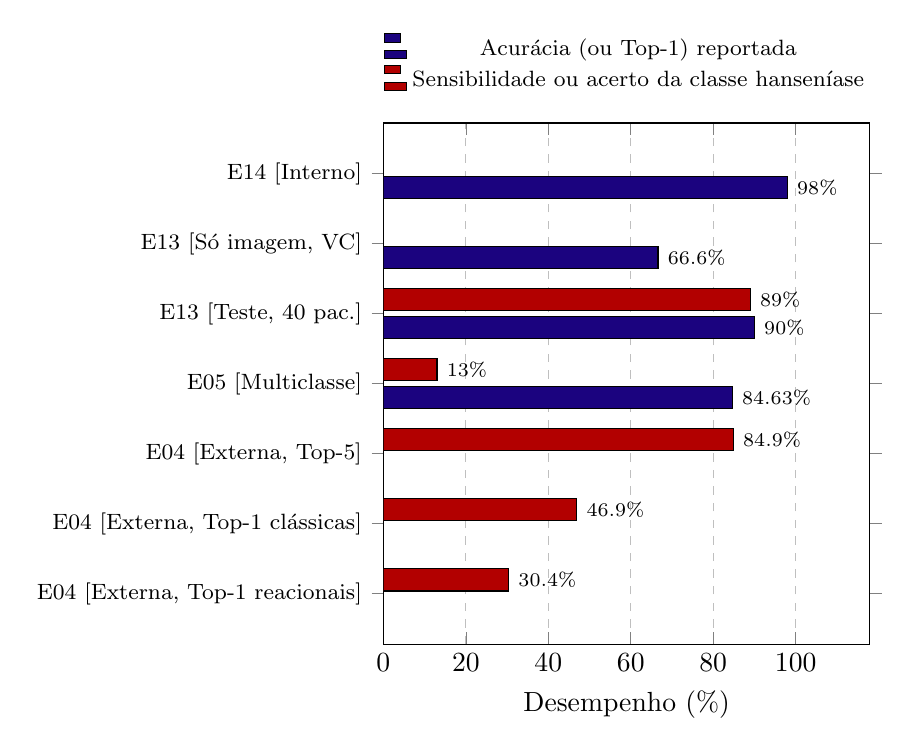
\begin{tikzpicture}
		\begin{axis}[
				xbar,
				width=0.64\textwidth,
				height=8.2cm,
				xmin=0, xmax=118,
				xlabel={Desempenho (\%)},
				symbolic y coords={
						{E04 [Externa, Top-1 reacionais]},
						{E04 [Externa, Top-1 clássicas]},
						{E04 [Externa, Top-5]},
						{E05 [Multiclasse]},
						{E13 [Teste, 40 pac.]},
						{E13 [Só imagem, VC]},
						{E14 [Interno]}
					},
				ytick={
						{E04 [Externa, Top-1 reacionais]},
						{E04 [Externa, Top-1 clássicas]},
						{E04 [Externa, Top-5]},
						{E05 [Multiclasse]},
						{E13 [Teste, 40 pac.]},
						{E13 [Só imagem, VC]},
						{E14 [Interno]}
					},
				yticklabel style={font=\footnotesize},
				nodes near coords={\pgfmathprintnumber\pgfplotspointmeta\%},
				nodes near coords align={horizontal},
				every node near coord/.append style={font=\scriptsize},
				bar width=8pt,
				enlarge y limits=0.12,
				xmajorgrids=true,
				grid style=dashed,
				legend style={at={(0.5, 1.04)}, anchor=south, legend columns=1, font=\footnotesize, draw=none}
			]
			\addplot[fill=blue!65!black, draw=black] coordinates {
					(98.0,{E14 [Interno]})
					(66.6,{E13 [Só imagem, VC]})
					(90.0,{E13 [Teste, 40 pac.]})
					(84.63,{E05 [Multiclasse]})
				};
			\addplot[fill=red!70!black, draw=black] coordinates {
					(89.0,{E13 [Teste, 40 pac.]})
					(13.0,{E05 [Multiclasse]})
					(84.9,{E04 [Externa, Top-5]})
					(46.9,{E04 [Externa, Top-1 clássicas]})
					(30.4,{E04 [Externa, Top-1 reacionais]})
				};
			\legend{Acurácia (ou Top-1) reportada, Sensibilidade ou acerto da classe hanseníase}
		\end{axis}
	\end{tikzpicture}
	\fonte{Autores, com os valores literais dos artigos (Tabela~\ref{tab:resultados-classificacao}). Barra ausente indica valor não reportado ou não verificado. \estudo{E05}: maior Top-1 (faixa de 76,61 a 84,63\%) e maior acerto da classe hanseníase (faixa de 12,0 a 13,0\%). \estudo{E04}: Top-1 por subconjunto, sem valor global. \estudo{E19} não aparece por não reportar acurácia de teste. VC: validação cruzada.}
\end{figure}

\subsection{Como o desempenho varia entre grupos ou tons de pele?}
\label{subsec:rq5-rq6-tom-pele}

As questões relativas à caracterização do tom de pele (RQ5) e à comparação de desempenho
entre diferentes fototipos cutâneos (RQ6) constituem o núcleo investigativo central deste
trabalho. A síntese dos 25 estudos incluídos mostra uma lacuna empírica: nenhum dos 16 estudos com dados
reporta, no texto principal, desempenho por tom de pele, e só três descrevem o tom de pele da base.

No que tange à caracterização do tom de pele (RQ5), três dos 16 estudos com dados descrevem a base,
em níveis diferentes. \estudo{E15} categoriza as imagens de treino em peles claras (4\%,
fototipos I-II), moderadas (26\%, III-IV) e escuras (70\%, V-VI) (Tabela 3 do artigo).
\estudo{E04} registra o fototipo de Fitzpatrick de 411 das 423 imagens (Tabela 1 do artigo; o
fototipo I não foi observado): nas lesões clássicas (subconjunto 1, 362 das 367 imagens com metadados), 1,1\% de fototipo II, 52,5\%
de III, 18,5\% de IV, 16,6\% de V e 11,3\% de VI; no subconjunto de reações e formas atípicas (n = 56),
7,1\% de II, 64,3\% de III, 8,9\% de IV, 0\% de V e 7,1\% de VI, com 12,5\% sem registro.
\estudo{E05} apenas afirma que todas as imagens são de populações africanas de pele escura,
com fototipo IV ou superior, sem apresentar a distribuição. Os outros 13 estudos com dados não informam
o tom de pele: cinco mencionam diversidade, limitação ou um campo de registro de tom sem apresentar dados
\estudo{E06,E13,E17,E18,E23},
e oito não o mencionam no texto principal
\estudo{E07,E08,E14,E19,E21,E22,E24,E25}.
No \textit{AI4Leprosy} \estudo{E13}, os autores descrevem imagens com ``diversidade de manifestações
clínicas e tipos de pele'', obtidas em um centro de referência nacional que recebe pacientes de todo o Brasil,
sem escala nem distribuição por tom. ``Não informa'' indica que o texto principal não traz dado utilizável
de tom de pele e não equivale a ``não avalia'', pois figuras e suplementos não foram examinados.

Quanto à variação do desempenho entre tons de pele (RQ6), nenhum dos 16 estudos com dados reporta, no
texto principal, métrica de acurácia, sensibilidade ou erro estratificada por tom de pele ou fototipo;
figuras e suplementos, como o de \estudo{E13}, não foram examinados. Mesmo nos estudos que
caracterizam o tom da base, o desempenho é apresentado de outra forma. \estudo{E15} reporta o teste
por doença, sem separar por faixa de tom, e reconhece que 96\% das imagens são de tom moderado ou escuro e
que o banco pode não ter o desempenho esperado em pacientes de pele clara. \estudo{E04} reporta o
desempenho por subconjunto (lesões clássicas, 87,2\% no Top-5, e reações ou formas atípicas, 69,6\%), cujas
composições de fototipo diferem; os autores indicam que essa composição pode ter influenciado os resultados,
de modo que a diferença está confundida com o tipo de lesão. Como a não informação do desempenho por tom não
equivale à sua ausência, a conclusão sustentada é que a evidência necessária não está disponível nos textos
principais dos estudos incluídos.

Esse vácuo de evidências contrasta com a revisão de \estudo{E16}, que, ao sintetizar outros
estudos, relata que modelos de aprendizado profundo, embora frequentemente acima de 85\% de acurácia em
dermatologia, apresentam de forma consistente pior desempenho em tons de pele escuros, com reduções de até
20\%, e discute o predomínio de tons mais claros nas bases usadas no desenvolvimento. Trata-se de afirmação de
revisão sobre outros estudos, e não de resultado dos estudos incluídos nesta revisão. Em doenças que cursam
com manchas hipocrômicas ou placas eritematosas,
é possível que a leitura de contraste entre a lesão e o tecido perilesional sádio dependa da
pigmentação basal do paciente, hipótese que os estudos incluídos não testam. A ausência de resultados estratificados nos textos principais impede
assegurar que os sistemas computacionais atuais operem de forma justa e segura na rede pública de saúde
do Brasil, justificando a urgência de protocolos de avaliação equitativos no SUS. A
Figura~\ref{fig:vazio-tom-pele} resume, para os 16 estudos com dados, quantos caracterizam o tom de pele da
base (RQ5) e quantos reportam desempenho por tom nos textos principais (RQ6).

\begin{figure}[htbp]
	\centering
	\caption{Caracterização do tom de pele (RQ5) e desempenho estratificado por tom (RQ6) nos 16 estudos com dados}
	\label{fig:vazio-tom-pele}
	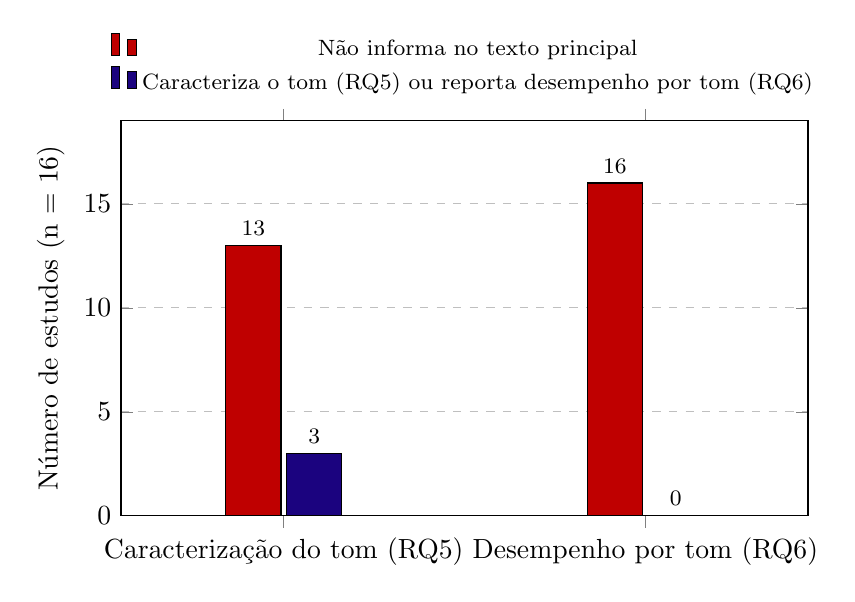
\begin{tikzpicture}
		\begin{axis}[
				ybar,
				width=0.85\textwidth,
				height=6.6cm,
				ymin=0, ymax=19,
				ylabel={Número de estudos (n = 16)},
				symbolic x coords={
						{Caracterização do tom (RQ5)},
						{Desempenho por tom (RQ6)}
					},
				xtick=data,
				nodes near coords,
				nodes near coords align={vertical},
				every node near coord/.append style={font=\footnotesize},
				bar width=20pt,
				enlarge x limits=0.45,
				ymajorgrids=true,
				grid style=dashed,
				legend style={at={(0.5, 1.04)}, anchor=south, legend columns=1, font=\footnotesize, draw=none}
			]
			\addplot[fill=red!75!black, draw=black] coordinates {
					({Caracterização do tom (RQ5)}, 13)
					({Desempenho por tom (RQ6)}, 16)
				};
			\addplot[fill=blue!65!black, draw=black] coordinates {
					({Caracterização do tom (RQ5)}, 3)
					({Desempenho por tom (RQ6)}, 0)
				};
			\legend{Não informa no texto principal, Caracteriza o tom (RQ5) ou reporta desempenho por tom (RQ6)}
		\end{axis}
	\end{tikzpicture}
	\fonte{Autores, a partir da leitura dos textos principais dos 16 estudos com dados (15 que desenvolvem modelo e a validação externa de \estudo{E04}); figuras e suplementos não foram examinados. ``Não informa'' não equivale a ``não avalia''. Em RQ5, três estudos caracterizam o tom da base em níveis diferentes: \estudo{E15} e \estudo{E04} com distribuição, e \estudo{E05} apenas pela afirmação de fototipo IV ou superior.}
\end{figure}

\subsection{Quais modelos e abordagens de inteligência artificial são empregados?}

Dos 25 estudos incluídos, 15 desenvolveram e avaliaram modelos, e \estudo{E04} avaliou independentemente um classificador existente. As frequências usam esses 16 estudos. As seis revisões, as duas perspectivas e o protocolo contribuem para a síntese narrativa. Cada publicação conta uma vez por modelo ou componente usado diretamente, incluindo comparadores testados e componentes de configurações avaliadas. Uma publicação pode contribuir para várias linhas.

A Tabela~\ref{tab:tarefas-ia} vincula as tarefas e as etapas dos sistemas aos estudos. O sistema de \estudo{E22} também descreve um classificador após a segmentação, com métricas apresentadas para o sistema. Em \estudo{E24}, o treino relatado para a classificação de gravidade abrange eczema e sarampo. A classificação de doenças desse estudo inclui hanseníase.

\begin{table}[htbp]
\centering
\small
\caption{Tarefas e etapas dos sistemas por estudo}
\label{tab:tarefas-ia}
\begin{tabular}{@{}>{\raggedright\arraybackslash}p{7.4cm}>{\raggedright\arraybackslash}p{6.3cm}@{}}
\toprule
\textbf{Tarefa ou etapa} & \textbf{Estudos} \\
\midrule
Classificação de doenças em imagens cutâneas & \estudo{E04,E05,E06,E07,E13,E14,E15,E17,E18,E19,E24,E25} \\
Classificação em microfotografias histopatológicas & \estudo{E08} \\
Detecção por caixas delimitadoras e classificação das lesões localizadas & \estudo{E23} \\
Segmentação binária de ferida e fundo & \estudo{E21,E22} \\
Delimitação da região de interesse como etapa da classificação & \estudo{E06,E07,E18} \\
Classificação após a segmentação como etapa do sistema & \estudo{E22} \\
Classificação de gravidade para eczema e sarampo & \estudo{E24} \\
\bottomrule
\end{tabular}
\fonte{Autores, a partir dos estudos incluídos.}
\end{table}

A Tabela~\ref{tab:abordagens-ia} e a Figura~\ref{fig:abordagens-ia} apresentam as abordagens. Cada estudo pode integrar várias categorias, inclusive pelo uso de comparadores testados. A abordagem híbrida exige que as técnicas coexistam na mesma configuração. O aprendizado profundo é contabilizado quando há evidência da profundidade da rede. A transferência de aprendizado foi usada, por exemplo, em \estudo{E05,E19,E24}, e o aprendizado com poucos exemplos em \estudo{E17}.

\begin{table}[htbp]
\centering
\small
\caption{Abordagens de IA identificadas nos estudos com avaliação de modelos}
\label{tab:abordagens-ia}
\begin{tabular}{@{}>{\raggedright\arraybackslash}p{3.2cm}>{\raggedright\arraybackslash}p{5.0cm}c>{\raggedright\arraybackslash}p{4.3cm}@{}}
\toprule
\textbf{Abordagem} & \textbf{Definição nesta análise} & \textbf{n/16} & \textbf{Estudos} \\
\midrule
Aprendizado profundo & Uso ou avaliação de redes profundas & 14/16 & \estudo{E04,E05,E06,E13,E14,E15,E17,E18,E19,E21,E22,E23,E24,E25} \\
Aprendizado tradicional & Classificadores tradicionais e vizinho mais próximo & 8/16 & \estudo{E06,E07,E08,E13,E17,E18,E22,E25} \\
Abordagem híbrida & Combinação de técnicas profundas e tradicionais ou de atributos aprendidos e manuais na mesma configuração & 5/16 & \estudo{E06,E13,E17,E18,E22} \\
Poucos exemplos & Estratégia \textit{few-shot} documentada & 1/16 & \estudo{E17} \\
\bottomrule
\end{tabular}
\fonte{Autores, a partir dos estudos incluídos.}
\end{table}

\begin{figure}[htbp]
\centering
\caption{Quantidade de estudos por abordagem de IA}
\label{fig:abordagens-ia}
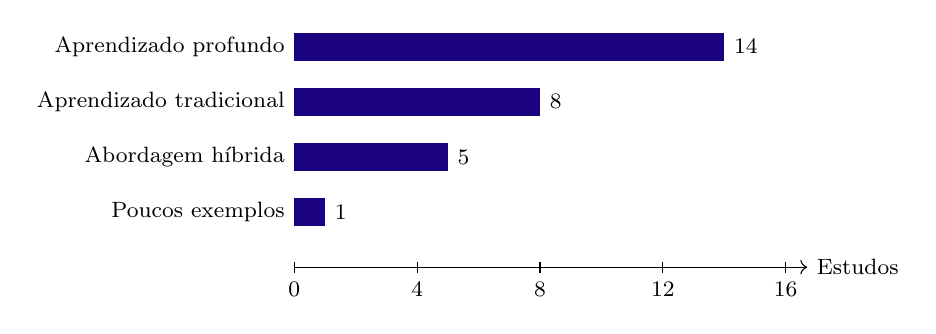
\begin{tikzpicture}[x=0.39cm,y=0.70cm]
\draw[->] (0,0) -- (16.7,0) node[right,font=\footnotesize] {Estudos};
\foreach \x in {0,4,8,12,16} {\draw (\x,0.1) -- (\x,-0.1) node[below,font=\footnotesize] {\x};}
\foreach \y/\n/\rotulo in {4/14/Aprendizado profundo,3/8/Aprendizado tradicional,2/5/Abordagem híbrida,1/1/Poucos exemplos} {
\fill[blue!65!black] (0,\y-0.25) rectangle (\n,\y+0.25);
\node[left,font=\footnotesize] at (0,\y) {\rotulo};
\node[right,font=\footnotesize] at (\n,\y) {\n};}
\end{tikzpicture}
\fonte{Autores, a partir dos 16 estudos com avaliação de modelos; categorias não exclusivas.}
\end{figure}

A Tabela~\ref{tab:modelos-resumo} apresenta os itens com pelo menos três ocorrências. O inventário auditado está na Tabela~\ref{tab:frequencia-modelos}, no Apêndice~\ref{apend:inventario-modelos}. A frequência mede o uso por publicação. A linha de U-Net inclui a adaptação de \estudo{E22}, a de ResNet-101 inclui seu uso como extrator ou codificador, e a de SVM reúne a variante multinível e a configuração otimizada por buraco negro.

\begin{table}[htbp]
\centering
\caption{Modelos e componentes com maior ocorrência nos estudos analisados}
\label{tab:modelos-resumo}
\begin{tabular}{@{}lcl@{}}
\toprule
\textbf{Modelo ou componente} & \textbf{Estudos (n/16)} & \textbf{Identificadores} \\
\midrule
Random Forest & 4/16 & \estudo{E06,E08,E13,E18} \\
SVM / Multi-SVM & 4/16 & \estudo{E06,E07,E08,E25} \\
ResNet-101 & 3/16 & \estudo{E06,E21,E25} \\
VGG-16 & 3/16 & \estudo{E05,E19,E24} \\
U-Net, incluindo adaptação & 3/16 & \estudo{E06,E21,E22} \\
ANN, arquitetura não especificada & 3/16 & \estudo{E06,E07,E08} \\
\bottomrule
\end{tabular}
\fonte{Autores, a partir dos estudos incluídos.}
\end{table}

A Figura~\ref{fig:ocorrencias-modelos} compara a quantidade de estudos para os mesmos modelos ou componentes da Tabela~\ref{tab:modelos-resumo}. Um estudo pode contribuir para mais de uma barra; o comprimento da barra não representa frequência exclusiva nem desempenho.

\begin{figure}[htbp]
\centering
\caption{Quantidade de estudos por modelo ou componente selecionado}
\label{fig:ocorrencias-modelos}
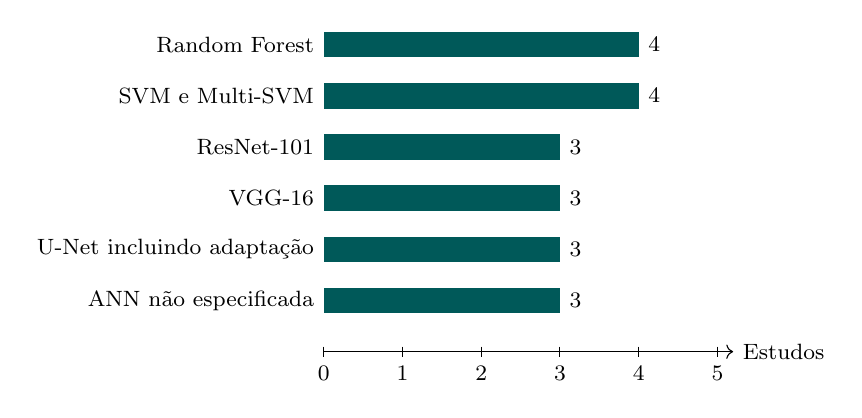
\begin{tikzpicture}[x=1.0cm,y=0.65cm]
\draw[->] (0,0) -- (5.2,0) node[right,font=\footnotesize] {Estudos};
\foreach \x in {0,1,2,3,4,5} {\draw (\x,0.1) -- (\x,-0.1) node[below,font=\footnotesize] {\x};}
\foreach \y/\n/\rotulo in {6/4/Random Forest,5/4/SVM e Multi-SVM,4/3/ResNet-101,3/3/VGG-16,2/3/U-Net incluindo adaptação,1/3/ANN não especificada} {
\fill[teal!70!black] (0,\y-0.25) rectangle (\n,\y+0.25);
\node[left,font=\footnotesize] at (0,\y) {\rotulo};
\node[right,font=\footnotesize] at (\n,\y) {\n};}
\end{tikzpicture}
\fonte{Autores, a partir dos 16 estudos com avaliação de modelos; categorias não exclusivas.}
\end{figure}

Entre os classificadores tradicionais, \estudo{E07} utilizou SVM otimizada, \estudo{E25} empregou Multi-SVM com descritores de textura e \estudo{E08} avaliou, entre outros, SVM, Random Forest e regressão logística em imagens histopatológicas. O XGBoost aparece entre os comparadores de \estudo{E13} e no classificador do sistema de \estudo{E22}. Duas atribuições permaneceram inconclusivas e ficaram fora da contagem: a árvore de decisão citada no texto de \estudo{E07} e a SVM citada na conclusão de \estudo{E19}.

Em \estudo{E13}, as configurações multimodais testadas combinaram a saída do modelo de imagens com a saída do modelo de características clínicas da lesão, dados do paciente ou ambos. A regressão logística elastic-net selecionada para o modelo final usa a saída do modelo de características clínicas da lesão e dados do paciente. Em \estudo{E17}, o protocolo de aquisição incluiu câmera, polarização e smartphone. O agrupamento de Ward formou subclasses para o experimento, e a rede siamesa operou sobre pares de imagens. A fusão dos modos de captura na entrada da rede fica indeterminada.

Quanto à atenção, \estudo{E21} avaliou o encoder Transformer SegFormer em configurações de U-Net e FPN. Em \estudo{E22}, o MEPS usa atenção guiada pelo gradiente para a segmentação, e o HSTFC pondera por atenção a fusão de atributos profundos e manuais antes da classificação. \estudo{E23} relata autoatenção no detector comparador baseado em ViT. Os mapas de saliência do YOLOv8n são um recurso de explicabilidade. A implementação da cabeça Transformer atribuída ao YOLOv9t permanece incerta. Essas configurações documentam candidatos à análise experimental posterior.

A CNN avaliada em \estudo{E04} é o classificador do segundo estágio do aplicativo da OMS, com arquitetura específica não informada. \estudo{E15} descreve uma implementação com DenseNet-121, triagem binária e classificação entre 12 DTNs no segundo estágio.

As revisões \estudo{E01,E02,E09,E12} sintetizam aplicações de classificadores tradicionais, redes profundas e combinações de técnicas. Os estudos primários correspondentes documentam ResNet-50 e VGG-16 \estudo{E05}, a LeprosyNet \estudo{E14}, a rede siamesa com aprendizado com poucos exemplos \estudo{E17} e as combinações avaliadas pelo AI4Leprosy \estudo{E13}. As contagens atribuem essas ocorrências aos estudos que realizaram as avaliações.

Além das aplicações com imagens, as revisões \estudo{E09,E10} relatam estudos que aplicam classificadores, como Random Forest e SVM, a dados de vigilância e respostas a questionários. Tais aplicações ampliam o panorama da inteligência artificial na hanseníase, mas se distinguem dos modelos de visão computacional que analisam imagens.

No campo da explicabilidade, a revisão \estudo{E16} discute mapas de saliência, Grad-CAM, mapas de atenção e escores de confiança como recursos para interpretar ou apresentar as decisões dos modelos, e não como classificadores independentes. Parte da literatura reunida nessa revisão aborda condições dermatológicas além da hanseníase; por isso, seus achados não devem ser transferidos automaticamente para essa doença.

As perspectivas \estudo{E03,E20} discutem a inteligência artificial como apoio à triagem e à decisão clínica, bem como desafios de representatividade dos dados, privacidade e supervisão humana. Em \estudo{E20}, ressalta-se a importância da história clínica, do exame físico e de testes laboratoriais para a confirmação diagnóstica; como possibilidade futura, menciona-se o uso de imagens multiespectrais ou térmicas, sem avaliação própria dessas modalidades.

\estudo{E11} propõe avaliar prospectivamente a versão beta do aplicativo da OMS. O protocolo descreve duas CNNs em cascata, com arquitetura específica indeterminada. A primeira distingue 24 condições comuns e um grupo de 12 DTNs cutâneas. A segunda diferencia as 12 DTNs desse grupo. A árvore de decisão offline para sintomas é outro recurso do aplicativo. O artigo apresenta o plano de avaliação.

\subsection{Como a generalização dos modelos é avaliada?}

A avaliação crítica da generalização dos modelos representa um dos achados mais determinantes da presente revisão sistemática, evidenciando uma lacuna estrutural entre os desempenhos computacionais reportados em laboratório e a capacidade real de implantação clínica no Sistema Único de Saúde (SUS):

\begin{enumerate}
	\item \textbf{Hegemonia de Avaliações Internas:} Em 14 dos 15 estudos que desenvolvem e avaliam um modelo (Tabela~\ref{tab:procedimentos-avaliacao}), como \estudo{E08,E14,E18,E19,E25}, a validação dos modelos é conduzida unicamente por divisões internas da mesma base de dados (\textit{hold-out}, divisão por classes ou validação cruzada interna); apenas um estudo \estudo{E23} testa o modelo também em outra base. Nesse desenho, treino e teste vêm da mesma coleta, o que impede avaliar o desempenho em outras condições de captura e pode mascarar fragilidades de sobreajuste (\textit{overfitting}).

	\item \textbf{Vazamento de Dados por Falta de Separação Estrita por Paciente:} A partição aleatória no nível de imagem (\textit{image-level split}), em vez de uma separação estrita por paciente (\textit{patient-level split}), é um risco de vazamento que não pode ser descartado: entre os 15 estudos que desenvolvem e avaliam um modelo, 13 não informam a unidade da separação (Tabela~\ref{tab:procedimentos-avaliacao}). Quando imagens de diferentes ângulos ou aproximações da mesma lesão pertencem simultaneamente aos conjuntos de treinamento e teste, o modelo decora artefatos de fundo e texturas superficiais do indivíduo, inflando artificialmente as métricas de acurácia.

	\item \textbf{Validação Externa Independente do Aplicativo da OMS:} A única validação externa independente de um modelo pré-treinado reportada nos estudos incluídos foi conduzida por \estudo{E04} com um banco de imagens clínicas de hanseníase coletadas entre 1996 e 2024. Ao submeter 423 imagens analisadas de um conjunto inicialmente composto por 439 imagens de 208 casos de hanseníase ao classificador de segundo estágio do aplicativo da OMS descrito no próprio estudo, os autores obtiveram sensibilidade Top-5 de 84,9\% (359 de 423 imagens). A sensibilidade Top-1 foi de 46,9\% nas lesões clássicas e de 30,4\% nas lesões reacionais ou atípicas, calculadas por subconjunto, sem valor global reportado, o que mostra que o resultado depende do número de predições consideradas.

	\item \textbf{Contribuição das Imagens e das Informações Clínicas (AI4Leprosy):} Em um único estudo \estudo{E13}, no teste com 40 pacientes, os modelos construídos só com as informações do paciente ou com as saídas do Modelo 2 (atributos clínicos da lesão) tiveram AUC superior a 90\%, enquanto as saídas do modelo de imagens, isoladas, tiveram AUC próxima de 70\%; para a floresta aleatória e o XGBoost, os autores relatam pouco benefício em acrescentar as saídas dos Modelos 1 e 2 às informações do paciente. A acurácia de 66,6\% do modelo de imagens vem de validação cruzada nos 182 pacientes de desenvolvimento, e a de 90\% do modelo final vem do teste de 40 pacientes; os procedimentos são distintos e os valores não são comparáveis diretamente. Por se tratar de um único estudo, com 40 pacientes de teste, não é possível concluir sobre um limite de desempenho da generalização fotográfica.

	\item \textbf{Ausência de Resultados de Aplicação em Serviço de Saúde:} Entre os 16 estudos com dados, nenhum reporta resultados de aplicação em serviço de saúde: as avaliações usam bancos de imagens pré-coletados, a validação externa de \estudo{E04} é retrospectiva, e \estudo{E15} trata a validação externa e a clínica como trabalho futuro. O único estudo que planeja avaliar o aplicativo da OMS em pacientes é o protocolo de \estudo{E11} no Senegal, ainda sem resultados.
\end{enumerate}

A Figura~\ref{fig:tipos-validacao} ilustra a distribuição dos 25 estudos incluídos quanto à abordagem de validação empregada: 14 avaliam o modelo somente na própria base, um testa também em outra base, um valida externamente um modelo de terceiros, um é protocolo sem resultados e oito são revisões, perspectivas ou editorial.

\begin{figure}[htbp]
	\centering
	\caption{Distribuição dos 25 estudos por abordagem de validação do modelo}
	\label{fig:tipos-validacao}
	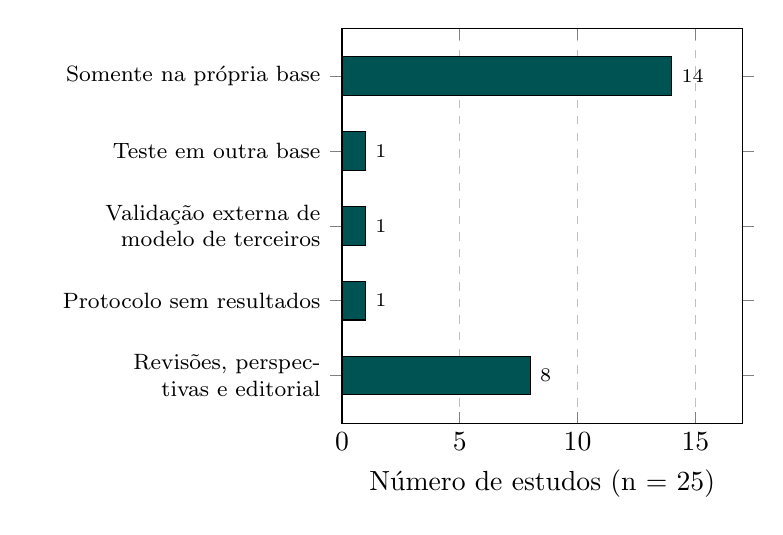
\begin{tikzpicture}
		\begin{axis}[
				xbar,
				width=0.55\textwidth,
				height=6.6cm,
				xmin=0, xmax=17,
				xlabel={Número de estudos (n = 25)},
				symbolic y coords={
						{Revisões, perspectivas e editorial},
						{Protocolo sem resultados},
						{Validação externa de modelo de terceiros},
						{Teste em outra base},
						{Somente na própria base}
					},
				ytick=data,
				yticklabel style={font=\footnotesize, text width=3.6cm, align=right},
				nodes near coords,
				nodes near coords align={horizontal},
				every node near coord/.append style={font=\scriptsize},
				bar width=14pt,
				enlarge y limits=0.16,
				xmajorgrids=true,
				grid style=dashed
			]
			\addplot[fill=teal!65!black, draw=black] coordinates {
					(8,{Revisões, perspectivas e editorial})
					(1,{Protocolo sem resultados})
					(1,{Validação externa de modelo de terceiros})
					(1,{Teste em outra base})
					(14,{Somente na própria base})
				};
		\end{axis}
	\end{tikzpicture}
	\fonte{Autores. Dos 15 estudos que desenvolvem modelo, 14 avaliam somente na própria base e um testa também em outra base \estudo{E23}; a validação externa de modelo de terceiros é a de \estudo{E04}; \estudo{E11} é um protocolo sem resultados; os oito restantes são seis revisões, uma perspectiva e um editorial.}
\end{figure}

\subsection{Em quais veículos os estudos são publicados?}

A distribuição dos 25 estudos incluídos quanto ao veículo de disseminação científica evidencia uma clara preponderância de periódicos indexados de alto fator de impacto sobre anais de congressos, além de demonstrar um notável caráter interdisciplinar entre as ciências da computação, a dermatologia e a saúde pública global:

\begin{itemize}
	\item \textbf{Periódicos Científicos (\textit{Journals}):} Totalizam 20 dos 25 estudos selecionados (80,0\% do corpo amostral). Essa concentração reflete o amadurecimento científico da temática e a necessidade de validação metodológica rigorosa por pares. Entre os periódicos da área médica, dermatológica e de saúde pública internacional, incluem-se veículos de prestígio como \textit{The Lancet Regional Health -- Americas} \estudo{E13}, \textit{PLOS Neglected Tropical Diseases} \estudo{E05}, \textit{Revista Panamericana de Salud Pública} \estudo{E04}, \textit{Journal of Investigative Dermatology} \estudo{E15}, \textit{International Health} \estudo{E20}, \textit{Frontiers in Medicine} \estudo{E03}, \textit{The American Journal of Dermatopathology} \estudo{E08}, \textit{Indian Journal of Leprosy} \estudo{E17}, \textit{Portuguese Journal of Dermatology and Venereology} \estudo{E09}, \textit{Journal of Clinical Medicine} \estudo{E01}, \textit{JMIR Research Protocols} \estudo{E11} e \textit{Malahayati International Journal of Nursing and Health Science} \estudo{E10}. No domínio da computação aplicada e bioinformática médica, destacam-se \textit{PLOS Computational Biology} \estudo{E02}, \textit{Engineering Applications of Artificial Intelligence} \estudo{E23}, \textit{BMC Artificial Intelligence} \estudo{E16}, \textit{Informatics in Medicine Unlocked} \estudo{E07}, \textit{SN Computer Science} \estudo{E06,E18,E25} e \textit{The International Journal of Lower Extremity Wounds} \estudo{E22}.

	\item \textbf{Anais de Conferências Internacionais (\textit{Conference Proceedings}):} Correspondem aos 5 estudos restantes (20,0\% da seleção), congregando trabalhos focados no desenvolvimento experimental rápido de novos modelos, segmentação de imagem e soluções de \textit{hardware} embarcado para a atenção periférica. Destacam-se eventos chancelados pelo IEEE: \textit{IEEE International Conference on Image Processing} (ICIP) \estudo{E21}, \textit{IEEE India Council International Conference} (INDICON) \estudo{E24}, \textit{IEEE International Conference on Computing, Communication and Networking Technologies} (ICCCNT) \estudo{E19}, \textit{IEEE International Conference on Emerging Trends in Computing and Communication} (ETCOM) \estudo{E12} e a \textit{International Conference on Sustainable Computing and Data Communication Systems} (ICSCDS) \estudo{E14}.
\end{itemize}

Por ano de publicação (Tabela~\ref{tab:estudos-incluidos}), há 1 estudo em 2021 (conferência), 2 em 2022 (revistas), 3 em 2023 (2 revistas e 1 conferência), 7 em 2024 (5 revistas e 2 conferências), 6 em 2025 (5 revistas e 1 conferência) e 6 em 2026 (todos em revistas). Entre 2021 e 2023, 4 dos 6 estudos foram publicados em revistas e 2 em anais de conferências; entre 2024 e 2026, 16 dos 19 em revistas e 3 em anais. A Figura~\ref{fig:veiculos-evolucao} apresenta essas contagens, com o ano impresso no PDF de cada artigo.

\begin{figure}[htbp]
	\centering
	\caption{Evolução temporal e distribuição dos 25 estudos por tipo de veículo de publicação (2021--2026)}
	\label{fig:veiculos-evolucao}
	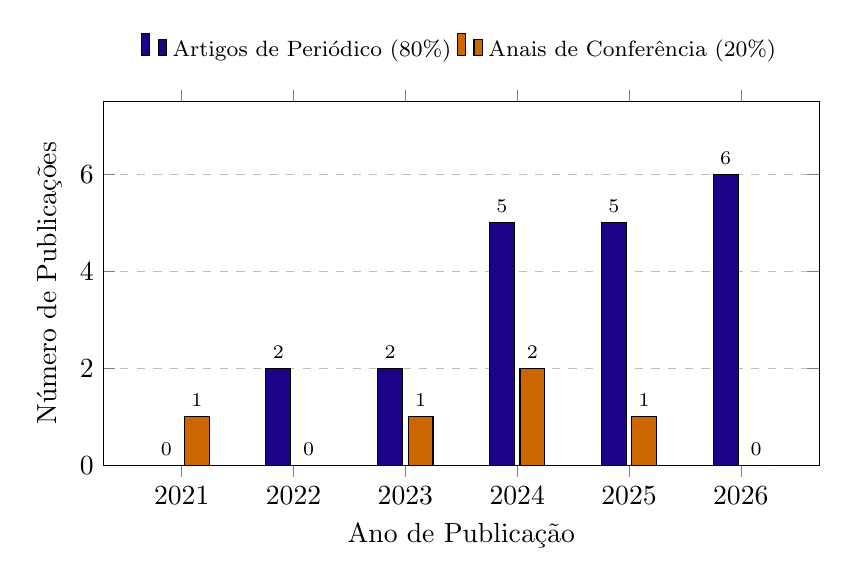
\begin{tikzpicture}
		\begin{axis}[
				ybar,
				width=0.88\textwidth,
				height=6.2cm,
				ymin=0, ymax=7.5,
				ylabel={Número de Publicações},
				xlabel={Ano de Publicação},
				symbolic x coords={2021, 2022, 2023, 2024, 2025, 2026},
				xtick=data,
				nodes near coords,
				every node near coord/.append style={font=\scriptsize},
				bar width=9pt,
				enlarge x limits=0.14,
				ymajorgrids=true,
				grid style=dashed,
				legend style={at={(0.5, 1.08)}, anchor=south, legend columns=2, font=\footnotesize, draw=none}
			]
			\addplot[fill=blue!70!black, draw=black] coordinates {
					(2021, 0)
					(2022, 2)
					(2023, 2)
					(2024, 5)
					(2025, 5)
					(2026, 6)
				};
			\addplot[fill=orange!80!black, draw=black] coordinates {
					(2021, 1)
					(2022, 0)
					(2023, 1)
					(2024, 2)
					(2025, 1)
					(2026, 0)
				};
			\legend{Artigos de Periódico (80\%), Anais de Conferência (20\%)}
		\end{axis}
	\end{tikzpicture}
	\fonte{Autores.}
\end{figure}

\bookmarksetup{startatroot}
\postextual
\bibliography{referencias_tcc}
\begin{apendicesenv}
\partapendices
% O ambiente apendicesenv e o \partapendices sao abertos em tcc.tex (um unico ambiente para este apendice e para notas.tex).
\chapter{Registros encontrados na busca}
\label{apend:registros}

Este apêndice lista os 118 registros que constam da etapa de busca e triagem, identificados sequencialmente de 1 a 118, com o identificador numérico (ID), o título, o ano, a fonte e a situação na triagem. Os registros que foram selecionados e confirmados para extração trazem também o identificador do estudo incluído (E01 a E25), que remete à Tabela~\ref{tab:estudos-incluidos}. Dos 118 registros, 91 foram excluídos na triagem por título e resumo, 26 foram selecionados para leitura integral (25 incluídos e um excluído em texto completo) e um apresentou decisão intermediária.

\begingroup
\scriptsize
\setlength{\tabcolsep}{2.5pt}
\renewcommand{\arraystretch}{1.1}
\begin{longtable}{@{}lp{6.4cm}lp{3.1cm}p{3.2cm}@{}}
\caption[Registros encontrados na busca (118 linhas das planilhas de triagem)]{Registros encontrados na busca (118 linhas das planilhas de triagem), com identificador (ID) e situa\c{c}\~ao}\label{tab:registros-118}\\
\toprule
\textbf{ID} & \textbf{T\'itulo} & \textbf{Ano} & \textbf{Fonte} & \textbf{Situa\c{c}\~ao} \\
\midrule
\endfirsthead
\multicolumn{5}{l}{\scriptsize\textit{Tabela~\ref{tab:registros-118} (continua\c{c}\~ao)}}\\
\toprule
\textbf{ID} & \textbf{T\'itulo} & \textbf{Ano} & \textbf{Fonte} & \textbf{Situa\c{c}\~ao} \\
\midrule
\endhead
\midrule
\multicolumn{5}{r}{\scriptsize\textit{continua na pr\'oxima p\'agina}}\\
\endfoot
\bottomrule
\endlastfoot
\hypertarget{estudo:1}{1} & Artificial Intelligence on Diagnostic Aid of Leprosy: A Systematic Literature Review & 2024 & Journal of Clinical Medicine & inclu\'ido (\estudo{E01}) \\
\hypertarget{estudo:2}{2} & On the usage of artificial intelligence in leprosy care: A systematic literature review & 2025 & PLOS Computational Biology & inclu\'ido (\estudo{E02}) \\
\hypertarget{estudo:3}{3} & The potential role of artificial intelligence in the clinical management of Hansen's disease (leprosy) & 2024 & Frontiers in Medicine & inclu\'ido (\estudo{E03}) \\
\hypertarget{estudo:4}{4} & Independent assessment of the WHO Skin Neglected Tropical Diseases application for leprosy detection & 2026 & Revista Panamericana de Salud Pública & inclu\'ido (\estudo{E04}) \\
\hypertarget{estudo:5}{5} & Deep learning for AI-based diagnosis of skin-related neglected tropical diseases: A pilot study & 2023 & PLOS Neglected Tropical Diseases & inclu\'ido (\estudo{E05}) \\
\hypertarget{estudo:6}{6} & Deep Semantic Segmentation Assisted Region-of-Interest Sensitive Deep Spatio-Textural Feature Learning Framework for Leprosy Detection and Classification & 2024 & SN Computer Science & inclu\'ido (\estudo{E06}) \\
\hypertarget{estudo:7}{7} & Skin Lesion Segmentation Based on Vision Transformers and Convolutional Neural Networks---A Comparative Study & 2022 & Applied Sciences & exclu\'ido na triagem \\
\hypertarget{estudo:8}{8} & Improving trust and confidence in medical skin lesion diagnosis through explainable deep learning & 2025 & International Journal of Data Science and Analytics & exclu\'ido na triagem \\
\hypertarget{estudo:9}{9} & Leprosy Screening Based on Artificial Intelligence: Development of a Cross-Platform App & 2021 & JMIR mHealth and uHealth & decis\~ao consolidada intermedi\'aria (M) \\
\hypertarget{estudo:10}{10} & Systematic review of deep learning image analyses for the diagnosis and monitoring of skin disease & 2023 & npj Digital Medicine & exclu\'ido na triagem \\
\hypertarget{estudo:11}{11} & Evaluating Machine Learning Models for Predicting Late Leprosy Diagnosis by Physical Disability Grade in Brazil (2018--2022) & 2025 & Tropical Medicine and Infectious Disease & exclu\'ido na triagem \\
\hypertarget{estudo:12}{12} & Assessment of Deep Learning Models for Cutaneous Leishmania Parasite Diagnosis Using Microscopic Images & 2023 & Diagnostics & exclu\'ido na triagem \\
\hypertarget{estudo:13}{13} & Retrospective validation of MetaSystems' deep-learning-based digital microscopy platform with assistance compared to manual fluorescence microscopy for detection of mycobacteria & 2024 & Journal of Clinical Microbiology & exclu\'ido na triagem \\
\hypertarget{estudo:14}{14} & Equity and Generalizability of Artificial Intelligence for Skin-Lesion Diagnosis Using Clinical, Dermoscopic, and Smartphone Images: A Systematic Review and Meta-Analysis & 2025 & Medicina & exclu\'ido na triagem \\
\hypertarget{estudo:15}{15} & Artificial Intelligence for the Classification of Pigmented Skin Lesions in Populations with Skin of Color: A Systematic Review & 2023 & Dermatology & exclu\'ido na triagem \\
\hypertarget{estudo:16}{16} & Improving Cross-Dataset Skin Lesion Segmentation with an Optimized U-Net++ Architecture & 2026 & 2026 IEEE 2nd International Conference on Quantum Photonics, Artificial Intelligence \&amp; Networking (QPAIN) & exclu\'ido na triagem \\
\hypertarget{estudo:17}{17} & Concordance of randomised controlled trials for artificial intelligence interventions with the CONSORT-AI reporting guidelines & 2024 & Nature Communications & exclu\'ido na triagem \\
\hypertarget{estudo:18}{18} & Quality assessment standards in artificial intelligence diagnostic accuracy systematic reviews: a meta-research study & 2022 & npj Digital Medicine & exclu\'ido na triagem \\
\hypertarget{estudo:19}{19} & Reporting guidelines in medical artificial intelligence: a systematic review and meta-analysis & 2024 & Communications Medicine & exclu\'ido na triagem \\
\hypertarget{estudo:20}{20} & Disparities in dermatology AI performance on a diverse, curated clinical image set & 2022 & Science Advances & exclu\'ido na triagem \\
\hypertarget{estudo:21}{21} & Optimized real-time diagnosis of neglected tropical diseases by automatic recognition of skin lesions & 2022 & Informatics in Medicine Unlocked & inclu\'ido (\estudo{E07}) \\
\hypertarget{estudo:22}{22} & Evaluating Advanced Machine Learning Models for Histopathological Diagnosis of Hansen Disease & 2025 & The American Journal of Dermatopathology & inclu\'ido (\estudo{E08}) \\
\hypertarget{estudo:23}{23} & Machine learning methods to predict leprosy misdiagnosis in Yunnan Province, People's Republic of China & 2026 & Frontiers in Public Health & exclu\'ido na triagem \\
\hypertarget{estudo:24}{24} & Unveiling leprosy through machines: a review of artificial intelligence in a neglected tropical disease & 2026 & Portuguese Journal of Dermatology and Venereology & inclu\'ido (\estudo{E09}) \\
\hypertarget{estudo:25}{25} & An mHealth App (eSkinHealth) for Detecting and Managing Skin Diseases in Resource-Limited Settings: Mixed Methods Pilot Study & 2023 & JMIR Dermatology & exclu\'ido na triagem \\
\hypertarget{estudo:26}{26} & Algorithm Design for a Cytokine Release Assay of Antigen-Specific In Vitro Stimuli of Circulating Leukocytes to Classify Leprosy Patients and Household Contacts & 2022 & Open Forum Infectious Diseases & exclu\'ido na triagem \\
\hypertarget{estudo:27}{27} & Enhancing Skin Lesion Diagnosis: Model Explainability Through Grad-CAM & 2026 & 2026 Second International Conference on Intelligent Systems for Communication, IoT and Security (ICISCoIS) & exclu\'ido na triagem \\
\hypertarget{estudo:28}{28} & Deep learning--based detection of acid-fast bacilli in microscopy images: a systematic review & 2026 & American Journal of Clinical Pathology & exclu\'ido na triagem \\
\hypertarget{estudo:29}{29} & Computer-Aided Bacillus Detection in Whole-Slide Pathological Images Using a Deep Convolutional Neural Network & 2020 & Applied Sciences & exclu\'ido na triagem \\
\hypertarget{estudo:30}{30} & Cross-Dataset and Demographic Validation of Proposed Model (SkinNetX): Ensuring Robustness, Fairness, and Clinical Readiness in Automated Skin Cancer Diagnosis & 2025 & 2025 2nd International Conference on Advanced Computing and Emerging Technologies (ACET) & exclu\'ido na triagem \\
\hypertarget{estudo:31}{31} & DSU-Net: Dual-Stage U-Net based on CNN and Transformer for skin lesion segmentation & 2025 & Biomedical Signal Processing and Control & exclu\'ido na triagem \\
\hypertarget{estudo:32}{32} & A novel end-to-end deep convolutional neural network based skin lesion classification framework & 2024 & Expert Systems with Applications & exclu\'ido na triagem \\
\hypertarget{estudo:33}{33} & Mapping and Quality Appraisal of Artificial Intelligence Preferential Reporting Checklists, Items, Guidelines, and Consensus in Healthcare: An Altmetric, Bibliometric, and Systematic Review & 2026 & International Journal of Dentistry & exclu\'ido na triagem \\
\hypertarget{estudo:34}{34} & Reducing skin tone bias in dermatology AI via sketch-guided multimodal fusion & 2026 & Scientific Reports & exclu\'ido na triagem \\
\hypertarget{estudo:35}{35} & Multi-Class Skin Lesion Classification Using a Lightweight Dynamic Kernel Deep-Learning-Based Convolutional Neural Network & 2022 & Diagnostics & exclu\'ido na triagem \\
\hypertarget{estudo:36}{36} & Mobile Health Strategies to Tackle Skin Neglected Tropical Diseases With Recommendations From Innovative Experiences: Systematic Review & 2020 & JMIR mHealth and uHealth & exclu\'ido na triagem \\
\hypertarget{estudo:37}{37} & Utilization of digital health in the screening, diagnosis, and management of Morbus Hansen & 2026 & Malahayati International Journal of Nursing and Health Science & inclu\'ido (\estudo{E10}) \\
\hypertarget{estudo:38}{38} & AI -generated dermatologic images show deficient skin tone diversity and poor diagnostic accuracy: An experimental study & 2025 & Journal of the European Academy of Dermatology and Venereology & selecionado para leitura; ausente das 25 extra\c{c}\~oes \\
\hypertarget{estudo:39}{39} & Self-supervised learning for medical image classification: a systematic review and implementation guidelines & 2023 & npj Digital Medicine & exclu\'ido na triagem \\
\hypertarget{estudo:40}{40} & The Development of a Mobile Application to Support Peripheral Health Workers to Diagnose and Treat People with Skin Diseases in Resource-Poor Settings & 2018 & Tropical Medicine and Infectious Disease & exclu\'ido na triagem \\
\hypertarget{estudo:41}{41} & Adaptation and performance of a mobile application for early detection of cutaneous leishmaniasis & 2021 & PLOS Neglected Tropical Diseases & exclu\'ido na triagem \\
\hypertarget{estudo:42}{42} & Potential of the World Health Organization's Skin NTDs App to Support and Improve the Detection of Skin-Related Neglected Tropical Diseases: Protocol for a Performance Evaluation and Feasibility Study in Senegal & 2025 & JMIR Research Protocols & inclu\'ido (\estudo{E11}) \\
\hypertarget{estudo:43}{43} & Self-Supervised Learning to Increase the Performance of Skin Lesion Classification & 2020 & Electronics & exclu\'ido na triagem \\
\hypertarget{estudo:44}{44} & GD03 Improving access to diagnosis and treatment of cutaneous neglected tropical diseases: a global health perspective & 2026 & British Journal of Dermatology & exclu\'ido na triagem \\
\hypertarget{estudo:45}{45} & Framework for developing explainable artificial intelligence models for neglected tropical disease diagnosis in low-resource settings & 2026 & Frontiers in Digital Health & exclu\'ido na triagem \\
\hypertarget{estudo:46}{46} & Quality of reporting of randomised controlled trials of artificial intelligence in healthcare: a systematic review & 2022 & BMJ Open & exclu\'ido na triagem \\
\hypertarget{estudo:47}{47} & Evaluating the World Health Organization's SkinNTDs App as a Training Tool for Skin Neglected Tropical Diseases in Ghana and Kenya: Cross-Sectional Study & 2024 & Journal of Medical Internet Research & exclu\'ido na triagem \\
\hypertarget{estudo:48}{48} & LSNet: a deep learning based method for skin lesion classification using limited samples and transfer learning & 2024 & Multimedia Tools and Applications & exclu\'ido na triagem \\
\hypertarget{estudo:49}{49} & Combining Artificial Intelligence and Simplified Image Processing for the Automatic Detection of Mycobacterium tuberculosis in Acid-fast Stain: A Cross-institute Training and Validation Study & 2024 & American Journal of Surgical Pathology & exclu\'ido na triagem \\
\hypertarget{estudo:50}{50} & Diagnosing skin neglected tropical diseases with the aid of digital health tools: A scoping review & 2024 & PLOS Digital Health & exclu\'ido na triagem \\
\hypertarget{estudo:51}{51} & Artificial Intelligence and Precision Dermatology across Inflammation, Cancer, and Infection: A Review & 2026 & Asian Pacific Journal of Cancer Care & exclu\'ido na triagem \\
\hypertarget{estudo:52}{52} & Leprosy & 1959 & Occupational Therapy: the Official Journal of the Association of Occupational Therapists & exclu\'ido na triagem \\
\hypertarget{estudo:53}{53} & Use of a convolutional neural network for direct detection of acid-fast bacilli from clinical specimens & 2025 & Microbiology Spectrum & exclu\'ido na triagem \\
\hypertarget{estudo:54}{54} & Disease Burden over Skin Tone: Decomposing the Dermatology-AI Generalization Gap & 2026 & não informado na fonte & exclu\'ido na triagem \\
\hypertarget{estudo:55}{55} & Deep Learning-Driven Skin Disease Detection and Classification System for Enhanced Medical Diagnosis & 2025 & 2025 1st International Conference on Advancement in Futuristic Technologies (ICAFT) & exclu\'ido na triagem \\
\hypertarget{estudo:56}{56} & An Integrated Deep Learning Model with EfficientNet and ResNet for Accurate Multi-Class Skin Disease Classification & 2025 & Diagnostics & exclu\'ido na triagem \\
\hypertarget{estudo:57}{57} & Differential diagnosis of acid-fast mycobacteria utilizing an artificial intelligence-based approach in histopathological analysis & 2026 & Diagnostic Pathology & exclu\'ido na triagem \\
\hypertarget{estudo:58}{58} & Artificial intelligence in clinical medicine: a state-of-the-art overview of systematic reviews with methodological recommendations for improved reporting & 2025 & Frontiers in Digital Health & exclu\'ido na triagem \\
\hypertarget{estudo:59}{59} & Evaluation of artificial intelligence-powered screening for sexually transmitted infections-related skin lesions using clinical images and metadata & 2024 & BMC Medicine & exclu\'ido na triagem \\
\hypertarget{estudo:60}{60} & Adapting Large Language Models to Mitigate Skin Tone Biases in Clinical Dermatology Tasks: A Mixed-Methods Study & 2025 & não informado na fonte & exclu\'ido na triagem \\
\hypertarget{estudo:61}{61} & A Machine Learning-Based Diagnosis of Leprosy: Study & 2025 & 2025 IEEE International Conference on Emerging Trends in Computing and Communication (ETCOM) & inclu\'ido (\estudo{E12}) \\
\hypertarget{estudo:62}{62} & A Deep Learning Approach for Automated Skin Lesion Diagnosis with Explainable AI & 2026 & não informado na fonte & exclu\'ido na triagem \\
\hypertarget{estudo:63}{63} & A multimodal transformer to fuse images and metadata for skin disease classification & 2023 & The Visual Computer & exclu\'ido na triagem \\
\hypertarget{estudo:64}{64} & Reimagining leprosy elimination with AI analysis of a combination of skin lesion images with demographic and clinical data. & 2022 & Lancet regional health. Americas & inclu\'ido (\estudo{E13}) \\
\hypertarget{estudo:65}{65} & Checklist for Evaluation of Image-Based Artificial Intelligence Reports in Dermatology: CLEAR Derm Consensus Guidelines From the International Skin Imaging Collaboration Artificial Intelligence Working Group. & 2022 & JAMA dermatology & exclu\'ido na triagem \\
\hypertarget{estudo:66}{66} & External Validation of AI Models for Skin Diseases: A Systematic Review & 2025 & IEEE Access & exclu\'ido na triagem \\
\hypertarget{estudo:67}{67} & Leprosy Diagnosis using Explainable Artificial Intelligence Techniques & 2023 & não informado na fonte & inclu\'ido (\estudo{E14}) \\
\hypertarget{estudo:68}{68} & Meta-Transfer Derm-Diagnosis: Exploring Few-Shot Learning and Transfer Learning for Skin Disease Classification in Long-Tail Distribution. & 2026 & IEEE journal of biomedical and health informatics & exclu\'ido na triagem \\
\hypertarget{estudo:69}{69} & Interpretable Deep Learning in Dermoscopy: An XAI-Driven Ensemble for Skin Lesion Diagnosis & 2026 & IEEE Access & exclu\'ido na triagem \\
\hypertarget{estudo:70}{70} & Lack of Transparency and Potential Bias in Artificial Intelligence Data Sets and Algorithms: A Scoping Review. & 2021 & JAMA dermatology & exclu\'ido na triagem \\
\hypertarget{estudo:71}{71} & The World Health Organization skin neglected tropical diseases app: A dynamic capacity-building training tool enhanced with artificial intelligence. & 2026 & The Journal of investigative dermatology & inclu\'ido (\estudo{E15}) \\
\hypertarget{estudo:72}{72} & Progressive Transfer Learning and Adversarial Domain Adaptation for Cross-Domain Skin Disease Classification. & 2019 & IEEE journal of biomedical and health informatics & exclu\'ido na triagem \\
\hypertarget{estudo:73}{73} & Development and validation of a machine learning approach for screening new leprosy cases based on the leprosy suspicion questionnaire. & 2025 & Scientific reports & exclu\'ido na triagem \\
\hypertarget{estudo:74}{74} & Performance Evaluation of No-Code Artificial Intelligence Models for the Detection of Acid-Fast Bacilli: A Comparative Analysis of Three Models. & 2024 & Cureus & exclu\'ido na triagem \\
\hypertarget{estudo:75}{75} & Dermatologist-level classification of skin cancer with deep neural networks. & 2017 & Nature & exclu\'ido na triagem \\
\hypertarget{estudo:76}{76} & Automated multi-class classification of skin lesions through deep convolutional neural network with dermoscopic images. & 2020 & Computerized medical imaging and graphics : the official journal of the Computerized Medical Imaging Society & exclu\'ido na triagem \\
\hypertarget{estudo:77}{77} & SkinDisNet: A comprehensive dataset of clinical images and metadata for skin disease detection and classification. & 2025 & Data in brief & exclu\'ido na triagem \\
\hypertarget{estudo:78}{78} & A novel integrated molecular and serological analysis method to predict new cases of leprosy amongst household contacts. & 2019 & PLoS neglected tropical diseases & exclu\'ido na triagem \\
\hypertarget{estudo:79}{79} & Explainable AI for differential diagnosis of skin-manifesting neglected tropical diseases (NTDS) in darker skin tones & 2026 & BMC Artificial Intelligence & inclu\'ido (\estudo{E16}) \\
\hypertarget{estudo:80}{80} & What is AI? Applications of artificial intelligence to dermatology. & 2020 & The British journal of dermatology & exclu\'ido na triagem \\
\hypertarget{estudo:81}{81} & Deep Learning for Diagnostic Binary Classification of Multiple-Lesion Skin Diseases. & 2020 & Frontiers in medicine & exclu\'ido na triagem \\
\hypertarget{estudo:82}{82} & EIU-Net: Enhanced feature extraction and improved skip connections in U-Net for skin lesion segmentation. & 2023 & Computers in biology and medicine & exclu\'ido na triagem \\
\hypertarget{estudo:83}{83} & Transparency in Artificial Intelligence Reporting in Ophthalmology-A Scoping Review. & 2024 & Ophthalmology science & exclu\'ido na triagem \\
\hypertarget{estudo:84}{84} & DEU-Net: Dual-Encoder U-Net for Automated Skin Lesion Segmentation & 2023 & IEEE Access & exclu\'ido na triagem \\
\hypertarget{estudo:85}{85} & Not-so-supervised: A survey of semi-supervised, multi-instance, and transfer learning in medical image analysis. & 2019 & Medical image analysis & exclu\'ido na triagem \\
\hypertarget{estudo:86}{86} & Leprosy Skin Lesion Detection: An AI Approach Using Few Shot Learning in a Small Clinical Dataset & 2023 & Indian Journal of Leprosy & inclu\'ido (\estudo{E17}) \\
\hypertarget{estudo:87}{87} & Skin Diseases Detection and Classification using Deep Learning Algorithm Convolutional Neural Network & 2017 & não informado na fonte & exclu\'ido na triagem \\
\hypertarget{estudo:88}{88} & Heuristic Segmentation Assisted Deep-Spatial Feature Learning Model for Leprosy Detection & 2024 & SN Computer Science & inclu\'ido (\estudo{E18}) \\
\hypertarget{estudo:89}{89} & Explainable deep inherent learning for multi-classes skin lesion classification & 2024 & Applied Soft Computing & exclu\'ido na triagem \\
\hypertarget{estudo:90}{90} & Leprosy lesion recognition using convolutional neural networks & 2016 & 2016 International Conference on Machine Learning and Cybernetics (ICMLC) & exclu\'ido na triagem \\
\hypertarget{estudo:91}{91} & Enhancing Diagnosis of Infectious Skin Disease: A Professional Approach using Deep Learning for Leprosy Detection & 2024 & 2024 15th International Conference on Computing Communication and Networking Technologies (ICCCNT) & inclu\'ido (\estudo{E19}) \\
\hypertarget{estudo:92}{92} & Harnessing artificial intelligence for skin-related neglected tropical diseases (skin NTDs): opportunities, challenges and future directions & 2025 & International Health & inclu\'ido (\estudo{E20}) \\
\hypertarget{estudo:93}{93} & Fusion of U-Net and CNN model for segmentation and classification of skin lesion from dermoscopy images & 2023 & Expert Systems with Applications & exclu\'ido na triagem \\
\hypertarget{estudo:94}{94} & Skin Lesion Segmentation based on Integrating EfficientNet and Residual block into U-Net Neural Network & 2020 & 2020 5th International Conference on Green Technology and Sustainable Development (GTSD) & exclu\'ido na triagem \\
\hypertarget{estudo:95}{95} & Automatic skin lesion segmentation using attention residual U-Net with improved encoder-decoder architecture & 2025 & Multimedia Tools and Applications & exclu\'ido na triagem \\
\hypertarget{estudo:96}{96} & Detection of Acid-Fast Bacilli AFB in Slit-Skin Smear Microscopy using MASK R-CNN Algorithm & 2023 & não informado na fonte & exclu\'ido na triagem \\
\hypertarget{estudo:97}{97} & Enhancing Medical Image Classification Using Self-Supervised Transfer Learning & 2024 & 2024 3rd International Conference for Innovation in Technology (INOCON) & exclu\'ido na triagem \\
\hypertarget{estudo:98}{98} & Comparison of Different Supervised and Self-supervised Learning Techniques in Skin Disease Classification & 2022 & não informado na fonte & exclu\'ido na triagem \\
\hypertarget{estudo:99}{99} & Fairness of Classifiers Across Skin Tones in Dermatology & 2020 & Lecture Notes in Computer Science & exclu\'ido na triagem \\
\hypertarget{estudo:100}{100} & Co2Wounds-V2: Extended Chronic Wounds Dataset from Leprosy Patients & 2024 & 2024 IEEE International Conference on Image Processing (ICIP) & inclu\'ido (\estudo{E21}) \\
\hypertarget{estudo:101}{101} & Integrative Image Processing Framework for Enhanced Detection of Leprosy-Associated Chronic Wounds & 2026 & The International Journal of Lower Extremity Wounds & inclu\'ido (\estudo{E22}) \\
\hypertarget{estudo:102}{102} & A trustworthy and explainable deep learning framework for skin lesion detection in smart dermatology & 2025 & Engineering Applications of Artificial Intelligence & inclu\'ido (\estudo{E23}) \\
\hypertarget{estudo:103}{103} & AI Driven Edge Device for Screening Skin Lesion and Its Severity in Peripheral Communities & 2021 & 2021 IEEE 18th India Council International Conference (INDICON) & inclu\'ido (\estudo{E24}) \\
\hypertarget{estudo:104}{104} & Skin Diseases Detection Using LBP and WLD: An Ensembling Approach & 2024 & SN Computer Science & inclu\'ido (\estudo{E25}) \\
\hypertarget{estudo:105}{105} & A Review of Software and Mobile Apps to Support the Clinical Diagnosis of Hansen Disease & 2023 & JMIR Dermatology & exclu\'ido na triagem \\
\hypertarget{estudo:106}{106} & Survey of Detection and Identification of Black Skin Diseases Based on Machine Learning & 2023 & Towards new e-Infrastructure and e-Services for Developing Countries & exclu\'ido na triagem \\
\hypertarget{estudo:107}{107} & Characteristics of publicly available skin cancer image datasets: a systematic review & 2022 & The Lancet Digital Health & exclu\'ido na triagem \\
\hypertarget{estudo:108}{108} & Skin Type Diversity in Skin Lesion Datasets: A Review & 2024 & Current Dermatology Reports & exclu\'ido na triagem \\
\hypertarget{estudo:109}{109} & Evaluating Deep Neural Networks Trained on Clinical Images in Dermatology with the Fitzpatrick 17k Dataset & 2021 & 2021 IEEE/CVF Conference on Computer Vision and Pattern Recognition Workshops (CVPRW) & exclu\'ido na triagem \\
\hypertarget{estudo:110}{110} & FairDisCo: Fairer AI in Dermatology via Disentanglement Contrastive Learning & 2023 & Computer Vision -- ECCV 2022 Workshops & exclu\'ido na triagem \\
\hypertarget{estudo:111}{111} & Fair and Accurate Skin Disease Image Classification by Alignment with Clinical Labels & 2024 & Medical Image Computing and Computer Assisted Intervention -- MICCAI 2024 & exclu\'ido na triagem \\
\hypertarget{estudo:112}{112} & PAD-UFES-20: A skin lesion dataset composed of patient data and clinical images collected from smartphones & 2020 & Data in Brief & exclu\'ido na triagem \\
\hypertarget{estudo:113}{113} & Automated Identification of Cutaneous Leishmaniasis Lesions Using Deep-Learning-Based Artificial Intelligence & 2023 & Biomedicines & exclu\'ido na triagem \\
\hypertarget{estudo:114}{114} & Harmonized Dual Deep Learning Architectures for Image-Based Diagnostics of Skin Neglected Tropical Diseases: Benchmark Study via Novel Funnel Framework & 2026 & JMIR Dermatology & exclu\'ido na triagem \\
\hypertarget{estudo:115}{115} & Artificial intelligence for the diagnosis of erythematous-squamous dermatological diseases: technological contributions to primary care & 2025 & Anais Brasileiros de Dermatologia & exclu\'ido na triagem \\
\hypertarget{estudo:116}{116} & The history of Teledermatology and its evolution, practical aspects, and prospects in Brazil & 2025 & Anais Brasileiros de Dermatologia & exclu\'ido na triagem \\
\hypertarget{estudo:117}{117} & Desenvolvimento e validação de chatbot para abordagem de lesões da hanseníase & 2026 & Ciência \& Saúde Coletiva & exclu\'ido na triagem \\
\hypertarget{estudo:118}{118} & Avaliação Automatizada de Qualidade e Adesão ao Protocolo de Aquisição de Imagens em Exames de Teledermatologia & 2024 & Anais Estendidos do Simpósio Brasileiro de Computação Aplicada à Saúde & exclu\'ido na triagem \\
\end{longtable}
\endgroup
\fonte{Autores.}


% Inventário de datasets da issue 28; fonte de trabalho: analises/issue-28-matriz-conferencia.md.
\chapter{Inventário dos conjuntos de dados e populações}
\label{apend:inventario-datasets}

O inventário relaciona cada estudo incluído ao conjunto de dados utilizado diretamente ou indica a ausência de amostra própria. A referência à página corresponde à posição no PDF consultado; os identificadores remetem à Tabela~\ref{tab:estudos-incluidos}. ``Não localizado'' indica que o dado não foi encontrado na consulta ao texto principal, sem afirmar que inexista. A disponibilidade é aquela declarada nas fontes e pode mudar. Imagens, pacientes, lesões, lâminas e anotações são unidades distintas.

\begingroup
\scriptsize
\setlength{\tabcolsep}{3pt}
\renewcommand{\arraystretch}{1.12}
\begin{longtable}{@{}>{\raggedright\arraybackslash}p{3.0cm}>{\raggedright\arraybackslash}p{9.0cm}>{\raggedright\arraybackslash}p{2.1cm}@{}}
\caption[Inventário dos datasets por estudo]{Inventário dos datasets e populações por estudo incluído}\label{tab:inventario-datasets}\\
\toprule
\textbf{Estudo e dataset} & \textbf{Origem, uso, amostra e disponibilidade} & \textbf{Fonte no PDF}\\
\midrule
\endfirsthead
\multicolumn{3}{l}{\scriptsize\textit{Tabela~\ref{tab:inventario-datasets} (continuação)}}\\
\toprule
\textbf{Estudo e dataset} & \textbf{Origem, uso, amostra e disponibilidade} & \textbf{Fonte no PDF}\\
\midrule
\endhead
\midrule
\multicolumn{3}{r}{\scriptsize\textit{continua na próxima página}}\\
\endfoot
\bottomrule
\endlastfoot
\estudo{E01}: Revisão sistemática & Síntese de estudos de IA em hanseníase; sem coleta primária. Não se aplica à amostra própria. Bases citadas não são atribuídas como dados próprios. & pp. 1--3 \\
\estudo{E02}: Revisão sistemática & Síntese de trabalhos sobre IA no cuidado da hanseníase; sem coleta primária. Não se aplica à amostra própria. Bases citadas são estudos secundários; não somar. & pp. 1--3 \\
\estudo{E03}: Perspectiva & Discussão sobre uso de IA na hanseníase; sem coleta primária. Não se aplica. Não se aplica à amostra própria. & p. 1 \\
\estudo{E04}: Conjunto externo sem nome & Curadoria independente UFES--OMS; avaliação externa de imagens de casos confirmados de hanseníase; país de coleta não explicitado. 439 imagens de 208 casos no conjunto inicial; 423 imagens analisadas após exclusão de 16; casos remanescentes e lesões únicas não informados. Idade, sexo e fototipo por imagem; acesso mediante solicitação ao autor. & pp. 1, 3--4, 6; Tabela 1 \\
\estudo{E05}: Coleção clínica sem nome & Costa do Marfim e Gana; treino e teste em hanseníase, úlcera de Buruli, micetoma, escabiose e bouba. 1.709 imagens de 506 pacientes; 131 imagens e 38 pacientes de hanseníase; lesões distintas não informadas. Autores descrevem fototipo IV ou superior sem distribuição; acesso institucional controlado. & pp. 1, 3--5; Tabela 1 \\
\estudo{E06}: Coleção clínica e fontes on-line & Hospitais, instituições de hanseníase e repositórios; país de coleta não localizado; classificação de hanseníase e pele normal. 220 imagens iniciais; 450 imagens de hanseníase após aumento/reapresentação; total de controles, pacientes e lesões únicas não localizado. Diversidade de cor mencionada sem distribuição; dados mediante solicitação razoável. & pp. 4, 15; seção Data Availability \\
\estudo{E07}: Coleção clínica sem nome & Camarões; colaboradores em Akonolinga; hanseníase, úlcera de Buruli e leishmaniose cutânea. 1.054 imagens: 372, 420 e 262 por condição; pacientes e lesões distintas não informados. Demografia e fototipo não informados; imagens por solicitação, características extraídas e código no GitHub. & pp. 4, 9--10; seção 2.1 \\
\estudo{E08}: Conjunto histopatológico sem nome & Instituto Colombiano de Medicina Tropical/Universidad CES; hanseníase e controles de pele saudável; treinamento e validação. 106 lâminas: 55 de pacientes com hanseníase e 51 de controles; 640 microfotografias (322 e 318). Distribuição demográfica, fototipo e condições de acesso não localizados. & pp. 1--2; Materials and Methods \\
\estudo{E09}: Revisão narrativa & Síntese de estudos sobre IA e hanseníase; sem coleta primária. Não se aplica à amostra própria. Bases citadas não são atribuídas como dados próprios. & p. 1 \\
\estudo{E10}: Revisão sistemática & Síntese de estudos sobre saúde digital e hanseníase; sem coleta primária. Não se aplica à amostra própria. Bases citadas não são atribuídas como dados próprios. & pp. 1--2 \\
\estudo{E11}: Coleta planejada no Senegal & Protocolo de avaliação do aplicativo da OMS; coleta prospectiva em Thiès. Meta de aproximadamente 800 imagens, não resultado; pacientes e lesões ainda não observados no protocolo. Acesso futuro mediante solicitação segundo o protocolo; não é uma base já coletada. & pp. 1, 4, 8; Sample Size \\
\estudo{E12}: Revisão de literatura & Revisão de aplicações de aprendizado de máquina na hanseníase. Não se aplica à amostra própria. Bases descritas pertencem aos estudos revisados. & pp. 1--2 \\
\estudo{E13}: AI4Leprosy & Fiocruz, Rio de Janeiro; desenvolvimento e teste interno com lesões suspeitas e outras dermatoses. Resultados: 1.226 imagens e 582 lesões de 222 pacientes. Distribuição numérica de fototipo não informada no texto principal; artigo descreve acesso mediante registro e validação. & pp. 1, 3--5, 8; Fig. 1 \\
\estudo{E14}: DermNet NZ e imagens da web & Conjunto curado para classificação de hanseníase versus não hanseníase; treino e teste. Quantidade total de imagens, pacientes e lesões únicas não localizada. Demografia e fototipo não localizados; DermNet/Kaggle e web citados como origem, acesso ao conjunto curado não localizado. & p. 2; seção III \\
\estudo{E15}: WHO Skin NTDs — imagens de DTNs & Imagens de DTNs cutâneas provenientes da OMS e de instituições parceiras; desenvolvimento e avaliação do classificador. 5.760 imagens; número de pacientes e de lesões distintas não localizado. A distribuição de tons é apresentada para 4.418 imagens de treino; acesso direto às imagens não localizado. & pp. 6, 8; Materials and Methods e Tabela 3 \\
\estudo{E15}: Fitzpatrick 17k — outras doenças & Atlas dermatológicos DermaAmin e Atlas Dermatologico; imagens de outras doenças cutâneas, excluídas as DTNs. 16.577 imagens; pacientes e lesões distintas não localizados. Acesso ao subconjunto utilizado não localizado; a fonte é identificada no artigo. & p. 6; Materials and Methods \\
\estudo{E15}: Recortes de pele saudável & Recortes de regiões saudáveis produzidos a partir das imagens de DTNs cutâneas. 2.469 recortes; número de imagens e pacientes originais correspondentes não localizado. São derivados de outra parcela da base e não equivalem a novos pacientes; acesso não localizado. & p. 6; Materials and Methods \\
\estudo{E15}: ImageNet — imagens não cutâneas & Imagens do ImageNet selecionadas para a categoria de conteúdo sem pele. 50.000 imagens não cutâneas; pacientes e lesões não se aplicam. Acesso ao subconjunto exato não localizado no artigo. & p. 6; Materials and Methods \\
\estudo{E16}: Revisão narrativa & Síntese de IA explicável e DTNs cutâneas em tons de pele escuros; sem coleta primária. Não se aplica à amostra própria. Bases citadas não são atribuídas como dados próprios. & p. 1 \\
\estudo{E17}: Coleção Sivananda Rehabilitation Home & Hyderabad/Telangana, Índia; lesões de hanseníase e condições semelhantes; desenvolvimento e teste. 1.931 imagens de 396 lesões, sendo 368 de hanseníase e 28 de outras condições, em 151 pacientes. Idade e sexo sem distribuição numérica localizada; acesso das imagens não localizado. & pp. 1, 3, 6; Materials and Methods \\
\estudo{E18}: Coleção clínica e fontes on-line & Hospitais e fontes secundárias; país de coleta não localizado; hanseníase e pele normal. 220 imagens iniciais; 450 imagens de hanseníase após processamento/anotação, conforme o artigo; pacientes, controles e lesões únicas não localizados. Diversidade de cor mencionada sem distribuição; dados mediante solicitação razoável. & pp. 5, 16; Data Availability \\
\estudo{E19}: Base curada Kaggle & Imagens de hanseníase tuberculoide; origem populacional não localizada; treino, validação e teste. Artigo informa 1.476 imagens no total, mas também 1.476 para treino, 62 para validação e 62 para teste; relação não esclarecida. Pacientes, lesões distintas e demografia não localizados; artigo aponta Kaggle. & p. 3; seção Dataset \\
\estudo{E20}: Perspectiva & Discussão sobre IA para DTNs cutâneas; sem coleta primária. Não se aplica à amostra própria. Bases citadas não são atribuídas como dados próprios. & pp. 1--3 \\
\estudo{E21}: Co2Wounds-V2 & Sanatorio de Contratación, Colômbia; imagens de feridas crônicas em pessoas com hanseníase; criação e benchmark. 764 imagens e 96 pacientes; 607 imagens de treino e validação anotadas; número de feridas únicas não localizado. 18 mulheres e 78 homens; idade média 75,5 $\pm$ 9,9 anos; Mendeley Data, versão 2. & pp. 1--2; seções 2.1--2.2 \\
\estudo{E22}: Co2Wounds-V2 & Mesmo dataset de E21; avaliação de processamento e segmentação de feridas crônicas. 764 imagens de 96 pacientes; 485 treino, 122 validação e 157 teste; não somar a E21. 18 mulheres e 78 homens; idade média 75,5 $\pm$ 9,9 anos; artigo aponta Mendeley Data. & pp. 7--8, 10--11; Tabelas 1--2 \\
\estudo{E23}: Fredrick Skin Disease Dataset & Roboflow; detecção de seis condições de pele, incluindo hanseníase; treinamento e avaliação. 1.101 imagens; 643 anotações de hanseníase; pacientes e lesões distintas não localizados. Origem geográfica e distribuição demográfica não localizadas; base descrita como pública. & pp. 4--5; seção 4 e Tabela 1 \\
\estudo{E23}: HAM10000 Skin Diseases Detection & Roboflow; teste entre bases de lesões cutâneas. Número de imagens efetivamente testadas e pacientes não localizado no artigo. Distribuição demográfica e origem da amostra analisada não localizadas; base descrita como pública. & p. 12; seção 6.2.3 \\
\estudo{E24}: Conjunto curado da web & Fontes abertas incluindo DermNet NZ e IEEE DataPort; eczema, sarampo, hanseníase e pele normal. 1.524 imagens; Tabela III: 51 sarampo, 1.235 eczema, 157 hanseníase e 81 pele normal; parágrafo próximo diverge em duas classes. Pacientes, lesões distintas e demografia não localizados; acesso ao conjunto curado não localizado. & pp. 4--5; seção Dataset e Tabela III \\
\estudo{E25}: JUCMATER: Skindb.v1 & School of Tropical Medicine, Calcutá, Índia; hanseníase, vitiligo, pitiríase versicolor e pele normal; treino e teste. 876 imagens de 141 pacientes; 262 imagens de hanseníase; número de lesões distintas não informado. Fototipo e distribuição demográfica não localizados; acesso para pesquisa mediante solicitação. & pp. 3, 8, 12; Data availability \\
\end{longtable}
\endgroup
\fonte{Elaboração própria a partir dos textos principais dos estudos incluídos. As condições de acesso são as descritas nas fontes consultadas.}

As contagens de \estudo{E21,E22} referem-se ao mesmo conjunto e não devem ser somadas. Nos estudos \estudo{E06,E18}, descrições semelhantes não bastam para estabelecer se as imagens são integralmente as mesmas. As diferenças de quantitativos em \estudo{E19,E24} são descritas na tabela. O protocolo \estudo{E11} contém uma meta de coleta, não uma amostra observada.

\section{Endereços e condições de acesso aos conjuntos}

Os endereços a seguir foram confrontados com as referências dos estudos e com as páginas dos provedores quando acessíveis em 13 de novembro de 2026. Um endereço da base de origem não identifica necessariamente as imagens selecionadas, a versão ou a partição utilizada pelos autores. As condições de acesso podem mudar.

\begin{itemize}
    \item \textbf{AI4Leprosy} \estudo{E13}: o artigo indica o identificador \url{https://doi.org/10.35078/1PSIEL} para o repositório e informa acesso mediante registro e validação. A página do Arca Dados foi acessada e identifica o artigo de \estudo{E13}; os arquivos podem estar sujeitos à solicitação de acesso.
    \item \textbf{Co2Wounds-V2} \estudo{E21,E22}: ambos os artigos apontam a versão 2 em \url{https://data.mendeley.com/datasets/s2w7rjwz49/2}. A página descreve 607 imagens anotadas para treino e validação e 157 imagens não anotadas para teste.
    \item \textbf{Fitzpatrick 17k} \estudo{E15}: repositório dos autores em \url{https://github.com/mattgroh/fitzpatrick17k}, com anotações e referências às imagens originais. A lista do subconjunto efetivamente empregado pela OMS não foi localizada.
    \item \textbf{ImageNet} \estudo{E15}: página geral de acesso em \url{https://www.image-net.org/download-images.php}; o artigo não identifica uma lista recuperável das 50.000 imagens selecionadas para a classe não cutânea.
    \item \textbf{Fredrick Skin Disease Dataset} \estudo{E23}: o próprio artigo indica \url{https://universe.roboflow.com/fredrick-gk-wpenz/skin-disease-hwlrn}. A página consultada descreve 1.101 imagens e seis classes, como no artigo; o conteúdo efetivamente processado deve ser conferido na versão disponibilizada.
    \item \textbf{Skin\_Diases\_Detection, referido como HAM10000} \estudo{E23}: o artigo referencia \url{https://universe.roboflow.com/universitas-dian-nuswantoro-u3s2y/skin_diases_detection}. A página foi identificada na indexação do provedor, mas sua abertura direta não foi possível nesta consulta; não foi confirmada a versão usada no teste. Esse endereço não deve ser confundido automaticamente com a versão integral original de HAM10000.
    \item \textbf{DermNet} \estudo{E14,E24}: o atlas citado está em \url{https://dermnetnz.org/}. Trata-se de uma fonte de imagens, não de um endereço confirmado para as coleções finais curadas em cada estudo.
    \item \textbf{Coleção de Camarões} \estudo{E07}: o artigo aponta \url{https://github.com/dodo12/MTNskin-Diagnosis} para as características extraídas. As imagens originais são disponibilizadas pelos autores mediante solicitação; o repositório de características não equivale ao conjunto de fotografias.
\end{itemize}

Para o conjunto externo ligado à UFES \estudo{E04}, a coleção de \estudo{E05}, os conjuntos de \estudo{E06,E18} e o JUCMATER: Skindb.v1 \estudo{E25}, os artigos indicam solicitação aos responsáveis, sem endereço público confirmado para as imagens. Nos demais conjuntos, inclusive a coleção de \estudo{E17}, a base de \estudo{E19} e os recortes usados em \estudo{E15}, não foi localizado um endereço verificável para a amostra exata. Em \estudo{E24}, a página do IEEE DataPort com nome semelhante foi localizada, mas o endereço impresso no artigo diverge e não permitiu confirmar que ela identifica a versão efetivamente utilizada.

% Frequências conferidas em analises/issue-29-matriz-modelos.md.
\chapter{Frequência dos modelos e componentes identificados}
\label{apend:inventario-modelos}
A tabela reúne modelos e componentes empregados nos 16 estudos com avaliação direta, incluindo comparadores testados, classificadores, segmentadores e extratores de atributos. Cada estudo contribui uma vez por item e pode aparecer em várias linhas. As versões não especificadas aparecem em linhas próprias. A matriz de conferência dos autores registra a função e a fonte de cada item.
\begingroup
\small
\setlength{\tabcolsep}{4pt}
\begin{longtable}{@{}>{\raggedright\arraybackslash}p{7.5cm}cp{4.5cm}@{}}
\caption{Modelos e componentes avaliados por estudo}\label{tab:frequencia-modelos}\\
\toprule
\textbf{Modelo ou componente} & \textbf{n} & \textbf{Estudos}\\
\midrule
\endfirsthead
\multicolumn{3}{l}{\small\textit{Tabela~\ref{tab:frequencia-modelos} (continuação)}}\\
\toprule
\textbf{Modelo ou componente} & \textbf{n} & \textbf{Estudos}\\
\midrule
\endhead
\midrule
\multicolumn{3}{r}{\small\textit{continua na próxima página}}\\
\endfoot
\bottomrule
\endlastfoot
Random Forest & 4 & \estudo{E06,E08,E13,E18} \\
SVM / Multi-SVM & 4 & \estudo{E06,E07,E08,E25} \\
ANN (não especificada) & 3 & \estudo{E06,E07,E08} \\
ResNet-101 & 3 & \estudo{E06,E21,E25} \\
U-Net (inclui adaptação) & 3 & \estudo{E06,E21,E22} \\
VGG-16 & 3 & \estudo{E05,E19,E24} \\
AlexNet & 2 & \estudo{E14,E18} \\
DenseNet-121 & 2 & \estudo{E15,E25} \\
Inception V3 & 2 & \estudo{E17,E24} \\
k-NN & 2 & \estudo{E06,E07} \\
Regressão logística (inclui elastic-net) & 2 & \estudo{E08,E13} \\
ResNet-50 & 2 & \estudo{E05,E13} \\
Árvore de decisão & 2 & \estudo{E06,E08} \\
XGBoost & 2 & \estudo{E13,E22} \\
CNN do aplicativo da OMS (segundo estágio) & 1 & \estudo{E04} \\
CNN extratora do HSTFC (arquitetura não especificada) & 1 & \estudo{E22} \\
CO-WinF & 1 & \estudo{E22} \\
DeepLabV3 & 1 & \estudo{E21} \\
DeepLabV3+ & 1 & \estudo{E21} \\
EfficientNet (versão não especificada) & 1 & \estudo{E21} \\
EfficientNet-B0 & 1 & \estudo{E19} \\
Faster R-CNN & 1 & \estudo{E23} \\
FPN & 1 & \estudo{E21} \\
Fuzzy C-Means com Firefly & 1 & \estudo{E18} \\
GoogLeNet & 1 & \estudo{E25} \\
Inception-v4 & 1 & \estudo{E13} \\
LeprosyNet & 1 & \estudo{E14} \\
MobileNet (versão não especificada) & 1 & \estudo{E25} \\
MobileNet v1 & 1 & \estudo{E19} \\
MobileNetV2 & 1 & \estudo{E24} \\
Naive Bayes & 1 & \estudo{E06} \\
Rede siamesa & 1 & \estudo{E17} \\
ResNet (versão não especificada) & 1 & \estudo{E14} \\
ResNet-152 & 1 & \estudo{E25} \\
ResNeXt-50 & 1 & \estudo{E21} \\
RetinaNet & 1 & \estudo{E23} \\
SegFormer & 1 & \estudo{E21} \\
Vision Transformer & 1 & \estudo{E23} \\
Vizinho mais próximo (1-NN) & 1 & \estudo{E17} \\
Xception (versão não especificada) & 1 & \estudo{E24} \\
Xception v1 & 1 & \estudo{E19} \\
YOLOv10n & 1 & \estudo{E23} \\
YOLOv8n & 1 & \estudo{E23} \\
YOLOv9t & 1 & \estudo{E23} \\
\end{longtable}
\fonte{Autores, a partir dos estudos incluídos.}
\endgroup

% !TeX root = ../tcc.tex
% O ambiente apendicesenv e o \partapendices sao abertos em tcc.tex.
\chapter{Notas para revisão com os orientadores --- fora do texto do capítulo}

\textbf{TCC de Euller e Gabriel · 15/10/2026}

Versão de trabalho baseada nas leituras fornecidas. A revisão da
literatura está em andamento. O texto abaixo é uma proposta de redação;
o contexto definido é o apoio à triagem de hanseníase na rede pública de
saúde do Brasil. O GQM e a questão de pesquisa foram atualizados
conforme a definição fornecida pela dupla. As notas editoriais ao final
não integram a introdução.

\section{Estrutura adotada e relação com os
exemplos}\label{estrutura-adotada-e-relauxe7uxe3o-com-os-exemplos}

Os três TCCs fornecidos organizam suas introduções em torno de contexto,
problema, questão de pesquisa, objetivos, organização/estrutura do
trabalho e cronograma. Esta versão desenvolve contexto, problema, GQM,
questão de pesquisa, objetivos e métricas. As métricas podem ser
deslocadas para o capítulo metodológico na organização final. A
organização dos capítulos e o cronograma devem refletir o planejamento
efetivamente aprovado, sem importar atividades experimentais dos
exemplos.

Os exemplos foram utilizados como referência de organização, não como
fontes científicas sobre hanseníase ou visão computacional. Não se
reproduziu o conteúdo temático desses trabalhos.

\section{Pontos que precisam de
decisão}\label{pontos-que-precisam-de-decisuxe3o}

\begin{itemize}
\tightlist
\item
  \textbf{Recorte territorial definido:} Brasil, no contexto da rede
  pública de saúde. Isso não implica que todos os estudos devam ser
  brasileiros ou que já exista validação local. Fundamentar
  posteriormente as particularidades do cenário brasileiro com fontes
  pertinentes.
\item
  \textbf{Escopo da questão:} ``como avaliar'' pode orientar uma
  proposta de avaliação mais ampla; a revisão responde inicialmente
  ``como os modelos têm sido avaliados''. Alinhar com os professores se
  a RQ central pertence ao TCC completo e as oito perguntas orientam a
  extração da revisão.
\item
  \textbf{Tons de pele:} o escopo passa a abranger imagens de pele em
  geral. A avaliação entre tons permanece em M6, quando houver
  evidências, sem restringir a questão central a pele negra. Fitzpatrick
  não equivale a identidade racial; origem geográfica não determina tom
  de pele.
\item
  \textbf{Contribuição do TCC 1:} a versão propõe síntese da literatura
  e fundamentação de avaliação futura. Não promete execução
  experimental, validação clínica ou aplicativo concluído nesta etapa.
\item
  \textbf{Fundamentação clínica:} para aprofundar definições, sinais
  diagnósticos ou epidemiologia, consultar fontes primárias/oficiais.
  Esta versão se limita ao contexto apresentado nos artigos e evita
  estatísticas epidemiológicas atuais não verificadas.
\item
  \textbf{Lacuna provisória:} as leituras permitem apontar questões de
  avaliação e relato. Não escrever que ``não existem estudos'' ou que a
  revisão já demonstrou uma lacuna definitiva enquanto a seleção e a
  extração não terminarem.
\end{itemize}

\section{Mapa das afirmações e das
fontes}\label{mapa-das-afirmauxe7uxf5es-e-das-fontes}

{\def\LTcaptype{none} % do not increment counter
\begin{longtable}[]{@{}
  >{\raggedright\arraybackslash}p{(\linewidth - 6\tabcolsep) * \real{0.2500}}
  >{\raggedright\arraybackslash}p{(\linewidth - 6\tabcolsep) * \real{0.2500}}
  >{\raggedright\arraybackslash}p{(\linewidth - 6\tabcolsep) * \real{0.2500}}
  >{\raggedright\arraybackslash}p{(\linewidth - 6\tabcolsep) * \real{0.2500}}@{}}
\toprule\noalign{}
\begin{minipage}[b]{\linewidth}\raggedright
Parte da redação
\end{minipage} & \begin{minipage}[b]{\linewidth}\raggedright
Base consultada
\end{minipage} & \begin{minipage}[b]{\linewidth}\raggedright
Onde conferir
\end{minipage} & \begin{minipage}[b]{\linewidth}\raggedright
Limite da afirmação
\end{minipage} \\
\midrule\noalign{}
\endhead
\bottomrule\noalign{}
\endlastfoot
Dificuldades de reconhecimento e panorama de IA & \estudo{E01} & Texto principal & Contextualização da revisão, sem números
atuais de prevalência \\
21 estudos e predominância de classificação multiclasse & \estudo{E01} & Resumo & Não significa 21 estudos elegíveis para o
protocolo de vocês \\
MobileNetV2 e protótipo Android & \estudo{E24} &
Resumo e introdução & Protótipo não equivale a validação clínica;
não afirmar estadiamento validado da hanseníase \\
CNNs e população de pele escura & \estudo{E05} & Texto principal & Dados
africanos não demonstram validação na rede pública brasileira \\
Resultados específicos de hanseníase & \estudo{E05} & Task 2/Figura 1 & 12\%/13\% são leitura da matriz por classe; não
misturar com Task 1 \\
Segmentação de feridas & \estudo{E21} & Texto principal &
Não é diagnóstico da hanseníase \\
YOLO e explicabilidade & \estudo{E23} & Texto principal & Mapas de
saliência não comprovam validade clínica \\
Diversidade limitada e validação prospectiva futura & \estudo{E23}
& Seções 6.4 e 7 & Não demonstra diferença quantitativa por tom
de pele \\
\end{longtable}
}

A conferência posterior do texto completo classificou \estudo{E12} como revisão da literatura. Pode apoiar o referencial e os trabalhos
relacionados; nesta introdução, priorizaram-se a revisão sistemática \estudo{E01} e os estudos primários fornecidos. Isso evita atribuir aos
revisores resultados que pertencem aos estudos citados.

\section{Situação do repositório
consultado}\label{situauxe7uxe3o-do-reposituxf3rio-consultado}

Consulta à branch \texttt{master} de \texttt{HansenSightAI/tcc}, em
14/10/2026. O arquivo \path{Monografia/editaveis/introducao.tex} ainda
contém uma introdução sobre análise de shaders em dispositivos móveis. O
arquivo \path{Monografia/bibliografia.bib} contém referências do mesmo
modelo de computação gráfica. Esta redação é um rascunho independente
para revisão; não foi aplicada ao repositório.

Caminhos consultados:

\begin{itemize}
\tightlist
\item
  https://github.com/HansenSightAI/tcc/blob/master/Monografia/editaveis/introducao.tex
\item
  https://github.com/HansenSightAI/tcc/blob/master/Monografia/bibliografia.bib
\end{itemize}

Na integração, substituir o texto do modelo pela versão aprovada e
acrescentar as referências abaixo. Antes de remover referências antigas,
verificar se ainda são citadas em outros capítulos do modelo.



\end{apendicesenv}
\end{document}
